\documentclass[11pt,a4paper]{article}

% ------------------------------------------------------------------
% Packages (same set as the main TSHC report)
% ------------------------------------------------------------------
\usepackage[T1]{fontenc}
\usepackage[utf8]{inputenc}
\usepackage{lmodern}
\usepackage{microtype}
\usepackage[a4paper,margin=2.5cm,headheight=14pt]{geometry}
\usepackage{amsmath,amssymb,amsthm,mathtools,bm}
\usepackage{graphicx}
\usepackage{booktabs,tabularx,multirow,longtable}
\usepackage{float}
\usepackage{xcolor}
\usepackage{enumitem}
\usepackage{fancyhdr}
\usepackage{caption}
\usepackage{algorithm}
\usepackage{algpseudocode}
\usepackage{tikz}
\usetikzlibrary{arrows.meta,positioning,shapes.geometric,fit,calc,backgrounds,decorations.pathreplacing}
\usepackage{tcolorbox}
\tcbuselibrary{skins,breakable}
\usepackage[round,authoryear]{natbib}
\usepackage[hidelinks]{hyperref}
\newcommand{\cref}[1]{\autoref{#1}}
\newcommand{\Cref}[1]{\autoref{#1}}
\renewcommand{\sectionautorefname}{Section}
\renewcommand{\subsectionautorefname}{Section}
\renewcommand{\subsubsectionautorefname}{Section}
\renewcommand{\equationautorefname}{Equation}
\renewcommand{\figureautorefname}{Figure}
\renewcommand{\tableautorefname}{Table}
\newcommand{\algorithmautorefname}{Algorithm}
\newcommand{\definitionautorefname}{Definition}
\newcommand{\propositionautorefname}{Proposition}

% ------------------------------------------------------------------
% Style (visual language of the main report)
% ------------------------------------------------------------------
\definecolor{accent}{HTML}{1F4E79}
\definecolor{soft}{HTML}{EAF1F8}
\definecolor{warnsoft}{HTML}{FFF4E5}
\definecolor{warnline}{HTML}{C77700}
\definecolor{measgreen}{HTML}{2E7D32}

\hypersetup{colorlinks=true,linkcolor=accent,citecolor=accent,urlcolor=accent,
  pdftitle={Entity-Centric Scientific Retrieval over a Temporal Knowledge Hypergraph},
  pdfauthor={Luka Burduli}}
\captionsetup{font=small,labelfont=bf}
\setlist{itemsep=2pt,topsep=4pt}
\renewcommand{\arraystretch}{1.15}
\setlength{\emergencystretch}{2em}
% Let figures share pages with text instead of occupying near-empty float pages
\renewcommand{\topfraction}{0.9}
\renewcommand{\bottomfraction}{0.8}
\renewcommand{\textfraction}{0.07}
\renewcommand{\floatpagefraction}{0.8}
\setcounter{topnumber}{3}
\setcounter{bottomnumber}{2}
\setcounter{totalnumber}{5}

\pagestyle{fancy}
\fancyhf{}
\fancyhead[L]{\small\textcolor{accent}{Entity-Centric Scientific Retrieval (V2 supplement)}}
\fancyhead[R]{\small\nouppercase{\leftmark}}
\fancyfoot[C]{\small\thepage}
\renewcommand{\headrulewidth}{0.4pt}

\newtheorem{definition}{Definition}[section]
\newtheorem{proposition}{Proposition}[section]
\theoremstyle{remark}
\newtheorem{remark}{Remark}[section]

\newtcolorbox{keybox}[1][]{colback=soft,colframe=accent,boxrule=0.6pt,arc=2pt,
  left=6pt,right=6pt,top=4pt,bottom=4pt,fonttitle=\bfseries\small,title={#1}}
\newtcolorbox{cautionbox}[1][]{colback=warnsoft,colframe=warnline,boxrule=0.6pt,arc=2pt,
  left=6pt,right=6pt,top=4pt,bottom=4pt,fonttitle=\bfseries\small,title={#1}}

\newcommand{\code}[1]{\texttt{\small #1}}
\newcommand{\R}{\mathbb{R}}
\DeclareMathOperator*{\argmax}{arg\,max}
\DeclareMathOperator{\RRF}{RRF}
\DeclareMathOperator{\rank}{rank}
\DeclareMathOperator{\simop}{sim}
\newcommand{\Ent}{\mathcal{E}}
\newcommand{\Ev}{\mathrm{Ev}}

\algrenewcommand\algorithmicrequire{\textbf{Input:}}
\algrenewcommand\algorithmicensure{\textbf{Output:}}

% Evidence-status tags used throughout the text
\newcommand{\vtag}[2]{{\sffamily\scriptsize\bfseries\textcolor{#1}{[#2]}}}
\newcommand{\Gtag}{\vtag{accent}{GUARANTEED}}
\newcommand{\Mtag}{\vtag{measgreen}{MEASURED}}
\newcommand{\Dtag}{\vtag{black!60}{DESIGN CHOICE}}
\newcommand{\Atag}{\vtag{warnline}{ASSUMED}}
\newcommand{\Otag}{\vtag{warnline}{DEVELOPMENT OBSERVATION}}

% Scale a picture down only if it is wider than the text block
\newcommand{\fitfig}[1]{\resizebox{\ifdim\width>\linewidth\linewidth\else\width\fi}{!}{#1}}

\tikzset{
  vbox/.style={draw=accent,fill=soft,rounded corners=3pt,align=flush center,inner sep=4pt},
  vwarn/.style={draw=warnline,fill=warnsoft,rounded corners=3pt,align=flush center,inner sep=4pt},
  vplain/.style={draw=gray!70,fill=white,rounded corners=3pt,align=flush center,inner sep=4pt},
  vdark/.style={draw=accent,fill=accent,text=white,rounded corners=3pt,align=flush center,inner sep=4pt},
  varr/.style={-{Stealth[length=2.2mm]},line width=0.8pt,draw=gray!70!black},
  vline/.style={line width=0.8pt,draw=gray!70!black},
  vlink/.style={line width=0.7pt,draw=accent,dashed}
}

% ------------------------------------------------------------------
\begin{document}
% ------------------------------------------------------------------

\hypersetup{pageanchor=false}
\begin{titlepage}
\centering
\vspace*{2.2cm}
{\color{accent}\rule{\linewidth}{1.2pt}}\\[0.8cm]
{\huge\bfseries Entity-Centric Scientific Retrieval over a\\[4pt] Temporal Knowledge Hypergraph\par}
\vspace{0.5cm}
{\Large A High-Recall Multi-Channel Retriever with\\ Cross-Encoder Reranking\par}
\vspace{0.6cm}
{\color{accent}\rule{\linewidth}{1.2pt}}\\[1.3cm]
{\large\textsc{Supplementary Technical Report}\par}
\vspace{0.25cm}
{\large Technical Supplement to \emph{Temporal Semantic Hypergraph Coarsening}\par}
\vspace{2.0cm}
{\Large Luka Burduli\par}
\vspace{0.4cm}
{\large October 2026\par}
\vfill
\begin{minipage}{0.84\linewidth}
\small\centering
Supplementary report for the downstream retrieval component, package
\code{clean\_tshc\_v2}. It explains the current V2 retrieval architecture
(configuration ``A6''), how every component works, how predictions are isolated from
ground truth, and what the frozen development results do and do not show.
It does \emph{not} replace the main TSHC report: the hierarchy, its guarantees and its
intrinsic evaluation are established there and are unchanged.
\end{minipage}
\vspace{1.5cm}
\end{titlepage}
\hypersetup{pageanchor=true}

% ------------------------------------------------------------------
\begin{abstract}
\noindent
The main report builds a laminar, budgeted, temporally regularised hierarchy over a
temporal knowledge hypergraph of 5{,}798 nodes and 1{,}429 hyperedges. Its extrinsic
evaluation exposed a separate problem: dense retrieval, flat or routed through the
hierarchy, found the right scientific \emph{region} but did not rank the exact answer
\emph{entity}; no expected method was recovered in the top 25. This supplement
describes the retrieval architecture built in response. It treats two tasks separately.
\emph{Candidate admission} forms a high-recall pool of canonical answer entities from six
inexpensive ranked lists (two dense views, BM25, safe name matching, evidence-to-entity
retrieval and bounded graph expansion), combined by reciprocal rank fusion.
\emph{Candidate ordering} scores only the first 100 fused candidates with a pretrained
relevance cross-encoder that reads the question together with an identity-first,
query-dependent evidence card of at most 512 tokens.

No model is trained and no weight or threshold is fitted; the one choice made with
development results in view is the reranking depth $K=100$. Predictions are produced in a
process that cannot read answers, are hashed, and are frozen before a separate evaluator
loads the ground truth. On the development benchmark (14 scored questions, 63 target
occurrences, 49 of them directly mapped to graph identities) the candidate pool admits
37 of 49 mapped targets, and the final ranking recovers 12 of 63 targets in the top 10,
18 in the top 25 and 37 in the top 100, with a mean reciprocal rank of 0.167. These are
development diagnostics on a benchmark that influenced design; they are not held-out
performance, and exact-answer ranking remains difficult.
\end{abstract}

\vspace{0.4cm}
\begin{keybox}[Scope of this document]
This document describes the current V2 retrieval architecture and its frozen development
results. It is intentionally scoped to that system rather than to the broader exploratory
history. Everything about the hierarchy itself (objective, laminarity, budgets,
coherence, hyperedge collapse, temporal identities, labels) is inherited from the main
report \citep{burduli2026tshc} and is only summarised here.
\end{keybox}

\clearpage
\tableofcontents
\clearpage
\listoffigures
\listoftables
\listofalgorithms
\clearpage

% ==================================================================
\section{Introduction}
\label{sec:intro}
% ==================================================================

\subsection{Motivation}

The assessment supplies a Temporal Knowledge Hypergraph (TKH) extracted from 52 papers on
machine-learning interatomic potentials and computational materials science. It has
5{,}798 nodes of twelve types (methods, techniques, components, cited works, claims,
tasks, problems, datasets, metrics, articles, authors, future topics) and 1{,}429
hyperedges of eleven relation types, with annual time stamps. The main report
\citep{burduli2026tshc} turns this graph into a three-level hierarchy of super-nodes at
four snapshots and evaluates that hierarchy intrinsically.

The assessment also asks whether the abstraction helps a \emph{downstream} task: given a
scientific question such as ``which methods are best suited for \dots'', find the
expected methods. The benchmark has 18 questions; 14 of them (Type~A) come with a list of
expected methods. This is the extrinsic part of task T6.

The main report ran that experiment honestly and reported a negative result. Under the
declared rule that the expected method's own node must appear in the top $k$, neither the
flat dense baseline nor any hierarchical beam recovered a single one of the 63 target
occurrences at $k=10$ or $k=25$. A positive control (forcing each mapped node to rank
one) recovered 49 of 49, so the evaluator was sound and the zero was a real property of
the retrieval design.

\subsection{Why V2 was needed}

The failure was not that retrieval found irrelevant material. The top results were
topically right: problem, task and claim nodes that paraphrase the question. What was
missing was the answer \emph{identity}. The main report's rank inspection makes this
concrete: for question Q1, the widely known potentials M3GNet, CHGNet, NequIP and MACE
sat at flat ranks 880, 1{,}340, 1{,}536 and 5{,}437 out of 5{,}480 documents.
\Mtag{} (main report)

\Cref{fig:failure} shows why. A long question is written in the vocabulary of problems,
requirements and outcomes. A claim or task node is written in the same vocabulary. A
method node is usually a short proper name. A single-vector similarity therefore ranks
the texts that \emph{describe} a solution above the name of the solution.

\begin{figure}[!htbp]
\centering
\fitfig{%
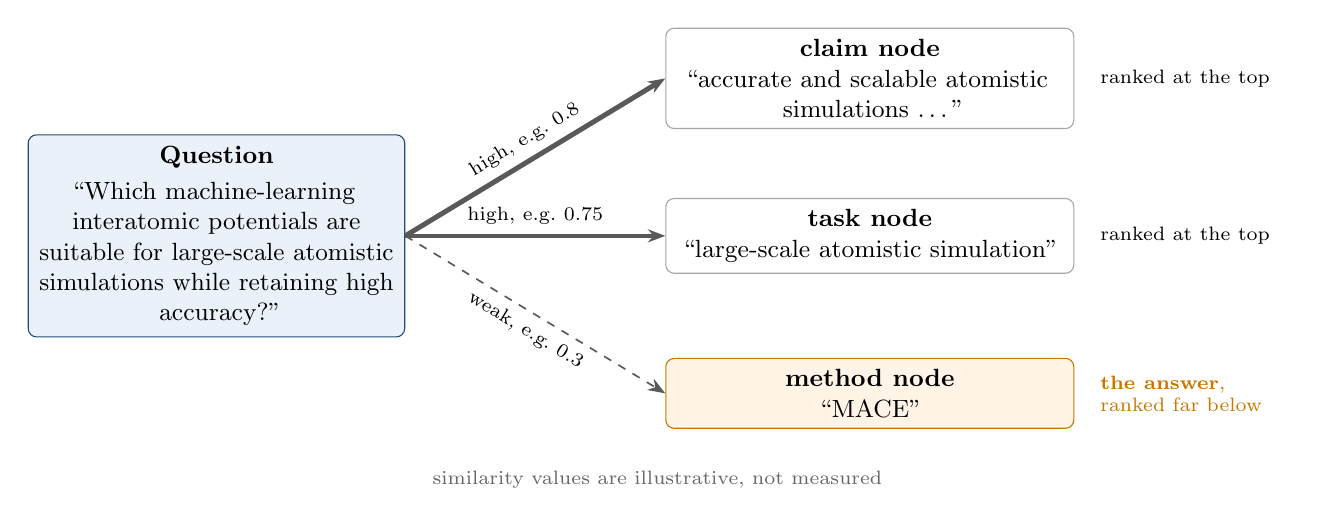
\begin{tikzpicture}[font=\small]
  \node[vbox,text width=4.5cm] (q) at (0,0) {\textbf{Question}\\[2pt]
    ``Which machine-learning interatomic potentials are suitable for large-scale
    atomistic simulations while retaining high accuracy?''};
  \node[vplain,text width=4.9cm,anchor=west] (c) at (5.7,2.0) {\textbf{claim node}\\
    ``accurate and scalable atomistic simulations \dots''};
  \node[vplain,text width=4.9cm,anchor=west] (t) at (5.7,0) {\textbf{task node}\\
    ``large-scale atomistic simulation''};
  \node[vwarn,text width=4.9cm,anchor=west] (m) at (5.7,-2.0) {\textbf{method node}\\
    ``MACE''};
  \draw[varr,line width=1.8pt] (q.east) -- node[above,sloped,font=\scriptsize] {high, e.g.\ 0.8} (c.west);
  \draw[varr,line width=1.5pt] (q.east) -- node[above,font=\scriptsize] {high, e.g.\ 0.75} (t.west);
  \draw[varr,line width=0.6pt,dashed] (q.east) -- node[below,sloped,font=\scriptsize] {weak, e.g.\ 0.3} (m.west);
  \node[anchor=west,font=\scriptsize,text width=2.5cm,align=flush left] at (11.1,2.0) {ranked at the top};
  \node[anchor=west,font=\scriptsize,text width=2.5cm,align=flush left] at (11.1,0) {ranked at the top};
  \node[anchor=west,font=\scriptsize,text width=2.5cm,align=flush left,text=warnline] at (11.1,-2.0)
     {\textbf{the answer},\\ ranked far below};
  \node[font=\scriptsize,text=black!60] at (5.6,-3.1)
     {similarity values are illustrative, not measured};
\end{tikzpicture}}
\caption[Why single-vector retrieval misses the answer identity]{Why single-vector retrieval misses the answer identity. A long question shares
its wording with claims and tasks, which describe the problem, far more than with a short
method name such as ``MACE''. Arrow thickness and the numbers are a schematic of cosine
similarity, labelled illustrative because they were not measured; the measured
consequence is the main report's rank inspection (MACE at flat rank 5{,}437 of 5{,}480 for
Q1). The texts that rank highest are evidence \emph{about} an answer, not the answer.}
\label{fig:failure}
\end{figure}

\begin{keybox}[The observation that motivates V2]
\centering
Semantic-region retrieval $\neq$ answer-identity retrieval.
\end{keybox}

The remedy is not a better similarity function applied to the same objects. It is to
change what is ranked and how evidence reaches it:

\begin{enumerate}
  \item rank \emph{answer entities}, not arbitrary graph nodes;
  \item let the informative texts (claims, tasks, problems) act as \emph{evidence that
        points to} an entity instead of competing with it;
  \item separate the cheap step that decides which entities are considered at all from
        the expensive step that orders them.
\end{enumerate}

The third point is the conceptual centre of this report. V2 separates
\textbf{candidate admission}, which must find a high-recall set of plausible answer
entities, from \textbf{candidate ordering}, which carefully reranks a much smaller set
using joint question--document interaction.

\subsection{V2 is a supplement, not a replacement}

V2 improves the \emph{extrinsic retrieval component} only. It does not replace or
redefine the TSHC objective, the hierarchy construction, P1 laminarity, P2 budgets, P3
semantic coherence, P4 native hyperedge collapse, P5 temporal regularisation and
persistent identities, or P6 label generation and held-out faithfulness evaluation. Those
are established by the main \code{clean\_tshc} system. V2 reads the same supplied TKH and
answers the same benchmark questions (\cref{fig:relation}).

\begin{figure}[!htbp]
\centering
\fitfig{%
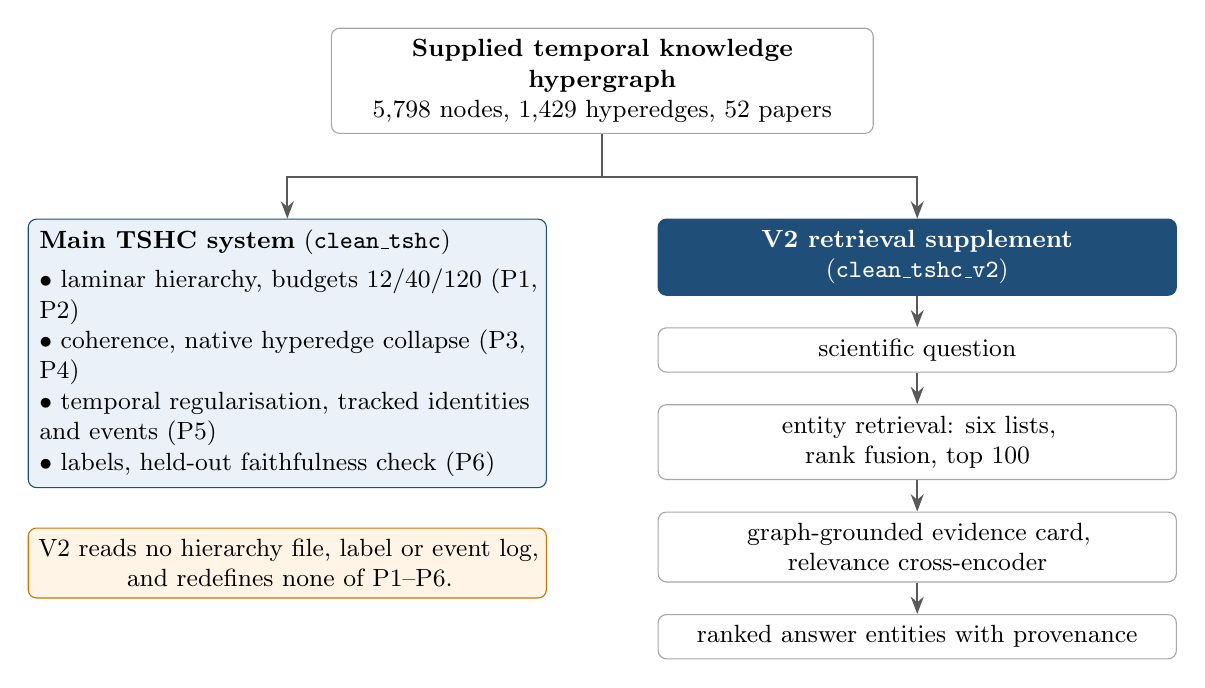
\begin{tikzpicture}[font=\small]
  \node[vplain,text width=6.6cm] (tkh) at (0,0) {\textbf{Supplied temporal knowledge hypergraph}\\
     5{,}798 nodes, 1{,}429 hyperedges, 52 papers};
  \node[vbox,text width=6.3cm,align=flush left,anchor=north] (main) at (-4.0,-1.75) {\textbf{Main TSHC system}
     (\texttt{clean\_tshc})\\[3pt]
     $\bullet$ laminar hierarchy, budgets 12/40/120 (P1, P2)\\
     $\bullet$ coherence, native hyperedge collapse (P3, P4)\\
     $\bullet$ temporal regularisation, tracked identities and events (P5)\\
     $\bullet$ labels, held-out faithfulness check (P6)};
  \node[vdark,text width=6.3cm,anchor=north] (v2) at (4.0,-1.75) {\textbf{V2 retrieval supplement}\\
     (\texttt{clean\_tshc\_v2})};
  \node[vplain,text width=6.3cm,below=4mm of v2] (s1) {scientific question};
  \node[vplain,text width=6.3cm,below=4mm of s1] (s2) {entity retrieval: six lists,\\ rank fusion, top 100};
  \node[vplain,text width=6.3cm,below=4mm of s2] (s3) {graph-grounded evidence card,\\ relevance cross-encoder};
  \node[vplain,text width=6.3cm,below=4mm of s3] (s4) {ranked answer entities with provenance};
  \node[vwarn,text width=6.3cm,below=5mm of main] (note) {V2 reads no hierarchy file, label or
     event log, and redefines none of P1--P6.};
  \draw[varr] (tkh.south) -- ++(0,-0.55) -| (main.north);
  \draw[varr] (tkh.south) -- ++(0,-0.55) -| (v2.north);
  \draw[varr] (v2) -- (s1); \draw[varr] (s1) -- (s2); \draw[varr] (s2) -- (s3); \draw[varr] (s3) -- (s4);
\end{tikzpicture}}
\caption[Relation between the main TSHC system and V2]{How the two packages relate. Both consume the same supplied hypergraph. The main
system produces the hierarchy and everything the assessment's properties P1--P6 refer to.
V2 is a separate downstream branch that answers the benchmark questions by retrieving
entities; it never reads the hierarchy's outputs, so it cannot alter them and cannot be
read as a competing clustering method.}
\label{fig:relation}
\end{figure}

\begin{cautionbox}[What V2's results cannot show]
Because V2 does not traverse the hierarchy, a gain in V2 retrieval is \emph{not}
evidence that the hierarchy helps retrieval. The main report's finding on that question
(research question RQ4: not demonstrated) stands unchanged.
\end{cautionbox}

\subsection{Contributions of V2}

\begin{itemize}
  \item \textbf{Canonical answer entities} instead of raw graph nodes, with conservative
        identity grouping and graph-supplied aliases (\cref{sec:entities}).
  \item \textbf{Six complementary first-stage lists}: two dense views, BM25, safe name
        matching, evidence-to-entity retrieval and bounded graph expansion
        (\cref{sec:channels}).
  \item \textbf{Evidence-to-entity retrieval}, which lets the texts that used to outrank
        the answer vote for it instead (\cref{sec:evidence-channel}).
  \item \textbf{Deterministic rank fusion} without score calibration or learned weights
        (\cref{sec:rrf}).
  \item \textbf{Query-dependent candidate evidence}: an identity-first card of selected,
        provenance-bearing evidence (\cref{sec:card}).
  \item \textbf{A genuine relevance cross-encoder} applied to the first 100 fused
        candidates (\cref{sec:crossencoder}).
  \item \textbf{A strict prediction/evaluation firewall}: predictions are hashed and
        frozen before the scorer can read the ground truth (\cref{sec:leakage}).
\end{itemize}

\subsection{How to read this document}

Statements are tagged where the distinction matters:
\begin{description}[leftmargin=0.6cm,style=nextline,itemsep=1pt]
  \item[\Gtag] Holds by construction of the algorithm or is enforced by code that fails
        loudly otherwise.
  \item[\Mtag] A number read from a frozen artifact of the run described in
        \cref{sec:repro}.
  \item[\Dtag] A fixed, declared setting chosen by judgement, not derived from data.
  \item[\Atag] Something the method relies on but that was not verified.
  \item[\Otag] A pattern seen on the development benchmark, which may not generalise.
\end{description}
``A6'' is the project's internal name for the configuration described here: the fused
candidate list reranked by the relevance cross-encoder, with a reranking pool of
$K=100$. That depth was selected after development results were available
(\cref{sec:k-status}).

% ==================================================================
\section{Relation to the Assessment Requirements}
\label{sec:assessment}
% ==================================================================

This section states exactly where each assessment requirement is satisfied, so that the
narrow scope of this supplement is not mistaken for an omission.

\subsection{Inherited guarantees: P1--P6}

The assessment defines six properties of a multi-resolution abstraction:

\begin{description}[leftmargin=1.2cm,style=nextline,itemsep=1pt]
  \item[P1] \textbf{Laminar refinement}: each level refines the one above it.
  \item[P2] \textbf{Size budget}: level $k$ has at most $N_k$ super-nodes; a hard constraint.
  \item[P3] \textbf{Semantic coherence}: members of a super-node are close in meaning.
  \item[P4] \textbf{Hyperedge fidelity}: the method works on the hypergraph and its
            coarsening rule is the one actually applied.
  \item[P5] \textbf{Temporal stability}: the hierarchy evolves smoothly and identities are
            trackable.
  \item[P6] \textbf{Interpretable, faithful labels}: labels assert nothing the members,
            visible at the cutoff, do not support.
\end{description}

All six are properties of a \emph{hierarchy}. V2 builds no hierarchy, so P1--P6 belong
entirely to the main system and V2 neither weakens nor alters them
(\cref{tab:p-mapping}). What V2 shares with them is discipline: it consumes the same
temporally valid graph data, keeps hyperedge provenance on every piece of evidence, and
does not reinterpret citation or structural context as scientific entailment.

\begin{table}[H]
\centering
\caption[Properties P1--P6 and their relation to V2]{Properties P1--P6: where each is established and what V2 has to do with it.
The middle column summarises the main report; nothing in it was re-run here.}
\label{tab:p-mapping}
\small
\begin{tabularx}{\linewidth}{lp{5.0cm}X}
\toprule
Requirement & Main TSHC responsibility & V2 relevance\\
\midrule
P1 Laminar refinement & Guaranteed by agglomerative, merge-only construction; tested &
  Unchanged. V2 builds no partition; entity grouping is not a multi-level hierarchy.\\
P2 Size budget & Fixed budgets of 12, 40 and 120 super-nodes; tested &
  Unchanged.\\
P3 Semantic coherence & Hierarchy objective; evaluated with an independent encoder
  against null partitions &
  Unchanged. Rank fusion combines retrieval signals; it is not a coherence measurement.\\
P4 Hyperedge fidelity & Native, multiplicity-preserving hyperedge collapse used by the
  objective &
  V2 uses graph-derived evidence and provenance read from native hyperedges; it does not
  redefine or perform the collapse.\\
P5 Temporal stability & Variation-of-information regularisation, Hungarian identity
  matching, event log &
  Snapshot validity is retained: the same visibility rule filters nodes and hyperedges.
  No new stability claim.\\
P6 Faithful labels & Label and gloss generation with held-out NLI checks &
  No change and no labels. V2 separately respects the temporal visibility of the evidence
  it shows.\\
\bottomrule
\end{tabularx}
\end{table}

\subsection{Tasks T1--T7}

\Cref{tab:t-mapping} does the same for the seven tasks. T6 is split into its six
evaluation requirements, because V2 changes exactly one of them: the extrinsic retrieval
experiment.

\begin{table}[!htbp]
\centering
\caption[Tasks T1--T7 and their relation to V2]{Tasks T1--T7. The six evaluation requirements inside T6 are listed separately
because only the last one is changed by V2.}
\label{tab:t-mapping}
\small
\begin{tabularx}{\linewidth}{p{3.7cm}p{4.9cm}X}
\toprule
Task & Covered in the main report by & This supplement\\
\midrule
T1 Evolving graph and data description & Per-snapshot counts, type and arity
  distributions, growth, data anomalies &
  Uses the same file and visibility rule; reports the retrieval index built from it
  (\cref{tab:index}).\\
T2 Formal method & Objective, structure/semantics trade-off, complexity, guarantees &
  Formal statement of the retrieval problem and ranking rule
  (\cref{sec:formulation} and \cref{sec:algorithm}), for the retrieval component only.\\
T3 Temporal coupling & Regularisation toward the previous snapshot; tracked identities &
  Unchanged. V2 applies one visibility cutoff per question (\cref{sec:temporal}).\\
T4 Hyperedge collapse & Collapse rule designed, implemented and used &
  Unchanged. V2 reads hyperedges with role checks; it coarsens nothing.\\
T5 Labels & Generated labels and glosses; measured faithfulness & Unchanged.\\
\midrule
T6 Coherence circularity issue & Different encoder for construction and for evaluation &
  Not applicable to V2 metrics, which are identity matches, not similarity scores. The
  analogous hazard for retrieval is leakage (\cref{sec:leakage}).\\
T6 Independent coherence evaluation & BGE-based coherence at three levels & Unchanged.\\
T6 Null models & 100 type- and size-preserving null partitions & Unchanged.\\
T6 Perturbation stability and confidence intervals & 10\% hyperedge deletion, five seeds,
  $t$-intervals; real cross-snapshot ARI & Unchanged. V2 reports point values only
  (\cref{sec:limitations}).\\
T6 Label overclaim evaluation & NLI check against held-out members & Unchanged.\\
T6 Extrinsic retrieval & Coarse-to-fine against flat; negative result reported &
  \textbf{Full detail in this document}: architecture, isolation, protocol, results.\\
\midrule
T7 Write-up; verified against assumed & Table of verified and assumed statements &
  Tags throughout and \cref{tab:verified}.\\
\bottomrule
\end{tabularx}
\end{table}

\subsection{Scoring criteria}

The assessment weights six criteria. \Cref{tab:weights} lists them with their weights and
shows which document carries the evidence for each.

\begin{table}[!htbp]
\centering
\caption[Scoring criteria and where they are addressed]{The assessment's scoring criteria and where each is addressed. The supplement
adds to the evaluation-validity and reproducibility evidence for the extrinsic task; the
hierarchy-specific criteria rest on the main report.}
\label{tab:weights}
\small
\begin{tabularx}{\linewidth}{p{3.9cm}rp{4.4cm}X}
\toprule
Criterion & Weight & Main report & This supplement\\
\midrule
Problem formulation and method design & 25\% & Objective, trade-off, guarantees against
  empirical properties & Retrieval problem formalised; each component's purpose stated
  (\cref{sec:formulation}--\cref{sec:card})\\
Evaluation validity & 30\% & Independent encoder, nulls, intervals, held-out labels,
  frozen predictions & Firewall and freeze (\cref{sec:leakage}), denominators and ceilings
  (\cref{sec:protocol}), development label (\cref{sec:results})\\
Temporal treatment & 15\% & Cross-snapshot stability and identity tracking & Visibility
  applied to nodes, edges and aliases (\cref{sec:temporal}); no new stability claim\\
Hyperedge collapse & 10\% & Rule and implementation (T4) & Not changed; hyperedges
  supply role-checked evidence (\cref{sec:temporal})\\
Reproducibility & 10\% & Commands, pinned dependencies, reruns & Pinned revisions, hashes,
  replay, tests (\cref{sec:repro})\\
Clarity; verified against assumed & 10\% & Verified/assumed table & Tags, caution boxes,
  \cref{tab:verified}\\
\bottomrule
\end{tabularx}
\end{table}

% ==================================================================
\section{Retrieval Problem Formulation}
\label{sec:formulation}
% ==================================================================

\subsection{Objects}

Let $H_t=(V_t,E_t)$ be the hypergraph snapshot visible at year $t$ (\cref{sec:temporal}).
A question is a string $q$. The retriever does not rank nodes; it ranks
\emph{canonical entities}.

\begin{definition}[Retrieval task]
\label{def:task}
Let $\Ent_t$ be the set of canonical entities of $H_t$ (\cref{def:entity}), let
$\Ent_t(q)\subseteq\Ent_t$ be the entities eligible for $q$ (\cref{def:eligible}), and
let $\Ev_t(e)$ be the graph-grounded evidence items linked to entity $e$. The task is to
produce an ordering
\begin{equation}
  \pi_q=(e_1,e_2,\dots,e_n),\qquad e_i\in\Ent_t(q),
\end{equation}
in which scientifically appropriate answer identities occur near the top, using only $q$,
$H_t$ and frozen pretrained models.
\end{definition}

\begin{table}[!htbp]
\centering
\caption[Notation]{Notation used in this report.}
\label{tab:notation}
\small
\begin{tabularx}{\linewidth}{lX}
\toprule
Symbol & Meaning\\
\midrule
$q$, $q_o$, $q_s$ & Question; its verbatim (original) view; its structured view\\
$H_t=(V_t,E_t)$ & Snapshot visible at year $t$\\
$\Ent_t$, $\Ent_t(q)$ & Canonical entities; those eligible for $q$\\
$\Ev_t(e)$ & Evidence items linked to entity $e$\\
$\phi(\cdot)\in\R^{384}$ & Unit-norm embedding from the frozen bi-encoder\\
$L_c$, $r_c(e)$ & Ranked list of channel $c$; rank of $e$ in it (from 1)\\
$F_q$ & Fused order of the union of all lists\\
$P_K(q)$ & Candidate pool: the first $K$ entities of $F_q$; here $K=100$\\
$s_{\mathrm{ce}}(q,e)$ & Cross-encoder relevance logit\\
$\pi_q$ & Final ranking\\
\bottomrule
\end{tabularx}
\end{table}

\subsection{Two stages, two metrics}

The system factorises as
\begin{equation}
  q\ \xrightarrow{\ \text{admission}\ }\ P_K(q)\ \xrightarrow{\ \text{ordering}\ }\ \pi_q .
\end{equation}
The stages have different goals and are measured differently. Let $\mathcal T$ be the
multiset of target occurrences (one per expected method per question) and
$\mathcal T_{\mathrm{dir}}\subseteq\mathcal T$ those mapped directly to graph identities
(\cref{sec:protocol}). Write $M(\tau)$ for the set of entities a mapped target $\tau$
resolves to.

\begin{definition}[Candidate recall]
\label{def:candrecall}
\begin{equation}
 \mathrm{CandidateRecall@}K=\frac{\bigl|\{\tau\in\mathcal T_{\mathrm{dir}}:\ M(\tau)\cap P_K(q_\tau)\neq\emptyset\}\bigr|}{|\mathcal T_{\mathrm{dir}}|}.
\end{equation}
Membership is measured on the pool \emph{before} reranking. The denominator is the
directly mapped occurrences (49 in the frozen evaluation).
\end{definition}

\begin{definition}[Final recall]
\label{def:recall}
With $\rank_{\pi}(\tau)=\min_{e\in M(\tau)}\rank_\pi(e)$,
\begin{equation}
 \mathrm{R@}k=\frac{\bigl|\{\tau\in\mathcal T_{\mathrm{dir}}:\ \rank_{\pi}(\tau)\le k\}\bigr|}{|\mathcal T|}.
\end{equation}
The numerator counts only directly mapped targets; the denominator is \emph{all} target
occurrences (63), so targets that cannot be mapped count as misses.
\end{definition}

The two denominators differ on purpose. Candidate recall asks ``of the answers that exist
in the graph, how many did stage one let through?''. Final recall asks ``of everything
the benchmark expects, how much did the system return?''. Both conventions are those of
the frozen evaluator.

\begin{proposition}[Admission is a ceiling]
\label{prop:ceiling}
Suppose the second stage only permutes $P_K(q)$ within the first $K$ positions and leaves
every other entity in fused order. Then for every $k\le K$ the number of targets
recovered at $k$ is at most the number admitted to the pool, and at $k=K$ the two are
equal, whatever scores the reranker assigns.
\end{proposition}
\begin{proof}
A target $\tau$ has $\rank_\pi(\tau)\le K$ exactly when some $e\in M(\tau)$ occupies one
of the first $K$ positions. Those positions hold precisely the entities of $P_K(q)$, in
some order. Hence $\rank_\pi(\tau)\le K$ iff $M(\tau)\cap P_K(q)\neq\emptyset$, and for
$k<K$ the condition can only be harder to meet.
\end{proof}

\begin{keybox}[Candidate admission is a ceiling]
A reranker cannot recover an entity that never enters its candidate pool. With $K=100$,
R@100 is fixed by the first stage alone \Gtag; the cross-encoder can only change which
admitted entities appear earlier.
\end{keybox}

This is why the two stages are logically distinct. Admission should be tolerant, because
its mistakes are final. Ordering should be discriminating, because it is the only place
where a precise judgement is affordable.

% ==================================================================
\section{Canonical Entity Representation}
\label{sec:entities}
% ==================================================================

\subsection{Why raw nodes are the wrong unit}

The graph often stores one scientific object as several nodes. A method can appear as a
\code{method} node extracted from the paper that proposes it, as a \code{cited\_work}
node from papers that cite it, and as a \code{component} node from a paper that uses it.
Ranking nodes would list the same answer several times, split its evidence, and make the
evaluation depend on which duplicate happens to be scored. V2 therefore groups nodes
into canonical entities before anything is ranked.

\subsection{Construction}

\begin{definition}[Canonical entity]
\label{def:entity}
Let $\nu$ be surface normalisation: Unicode NFKC, case-folding, mapping typographic
hyphens and the minus sign to ``-'', and collapsing whitespace. Let the family map send
the types \code{method}, \code{technique}, \code{component} and \code{cited\_work} to the
single family \emph{approach}, and each of \code{dataset}, \code{metric} and
\code{article} to itself. Two visible nodes $u,v$ of these seven types are equivalent
when they lie in the same family and
$\nu(\mathrm{surface}(u))=\nu(\mathrm{surface}(v))$. A canonical entity is an
equivalence class. Its identifier is formed from the lexicographically smallest member
node id; it records all member node ids, the set of member types, every distinct surface
form, the graph-provided aliases, the earliest \code{first\_seen\_year} among members and
each member's provenance.
\end{definition}

Three properties of this definition are deliberate. \Dtag
\begin{itemize}
  \item \textbf{Exact, not fuzzy.} Grouping needs equal normalised surface forms. No edit
        distance, embedding similarity or abbreviation expansion is used, because a wrong
        merge silently fuses two scientific objects.
  \item \textbf{Compatible family.} A dataset and a method that share a name stay separate
        entities. In the frozen index ``Materials Project'' is both an approach entity
        and a dataset entity. \Mtag
  \item \textbf{Aliases help retrieval but do not merge.} An alias stored in the graph is
        searchable text for the name and lexical channels. It never causes two entities
        with different surface forms to be joined.
\end{itemize}
Claims, tasks and problems are not answer entities; they are evidence
(\cref{sec:evidence-links}). Authors and future-topic nodes are neither.

\begin{figure}[!htbp]
\centering
\fitfig{%
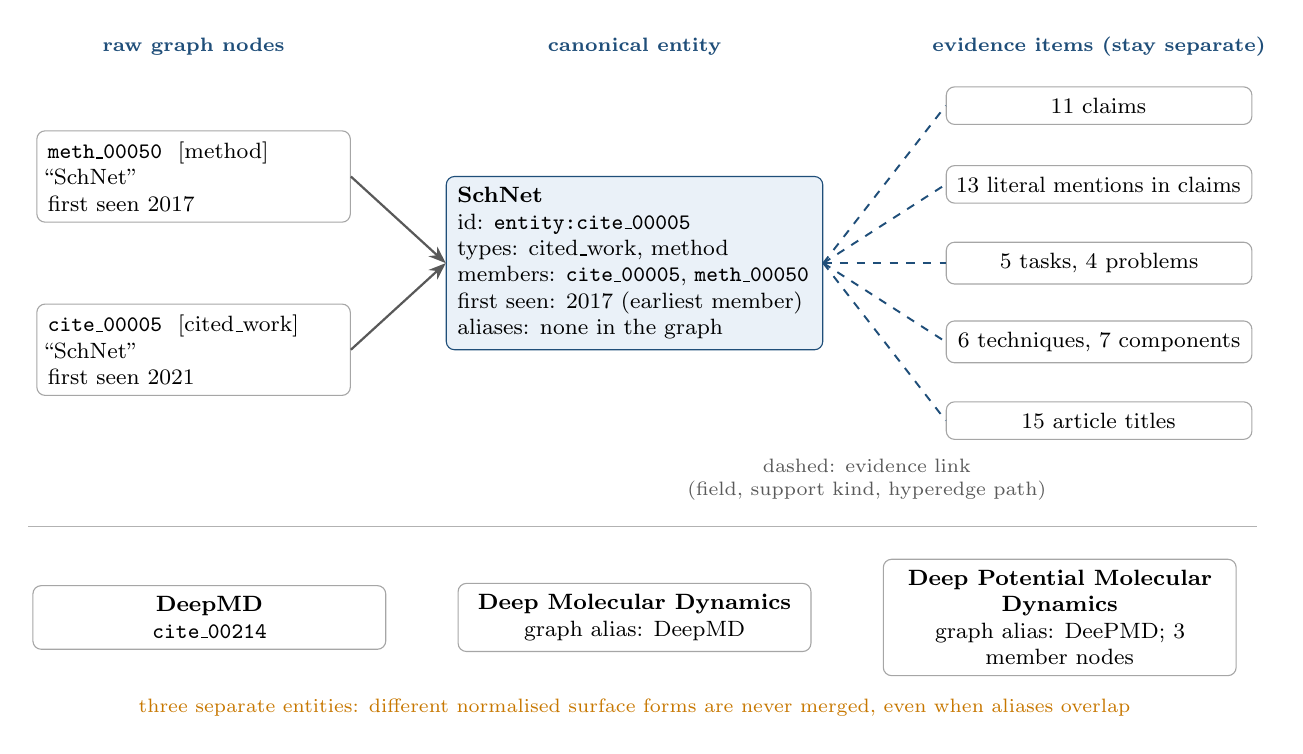
\begin{tikzpicture}[font=\footnotesize]
  \node[font=\scriptsize\bfseries,text=accent] at (0,2.75) {raw graph nodes};
  \node[font=\scriptsize\bfseries,text=accent] at (5.6,2.75) {canonical entity};
  \node[font=\scriptsize\bfseries,text=accent] at (11.5,2.75) {evidence items (stay separate)};
  \node[vplain,text width=3.7cm,align=flush left] (n1) at (0,1.1) {\texttt{meth\_00050}\ \ [method]\\ ``SchNet''\\ first seen 2017};
  \node[vplain,text width=3.7cm,align=flush left] (n2) at (0,-1.1) {\texttt{cite\_00005}\ \ [cited\_work]\\ ``SchNet''\\ first seen 2021};
  \node[vbox,text width=4.5cm,align=flush left] (e) at (5.6,0) {\textbf{SchNet}\\
     id: \texttt{entity:cite\_00005}\\ types: cited\_work, method\\
     members: \texttt{cite\_00005}, \texttt{meth\_00050}\\ first seen: 2017 (earliest member)\\
     aliases: none in the graph};
  \draw[varr] (n1.east) -- (e.west);
  \draw[varr] (n2.east) -- (e.west);
  \foreach \y/\txt/\nm in {2.0/{11 claims}/v1,1.0/{13 literal mentions in claims}/v2,
      0/{5 tasks, 4 problems}/v3,-1.0/{6 techniques, 7 components}/v4,-2.0/{15 article titles}/v5}{
    \node[vplain,text width=3.6cm] (\nm) at (11.5,\y) {\txt};
    \draw[vlink] (e.east) -- (\nm.west);
  }
  \node[font=\scriptsize,text=black!65,align=flush center] at (8.55,-2.75) {dashed: evidence link\\ (field, support kind, hyperedge path)};
  \draw[gray!60] (-2.1,-3.35) -- (13.5,-3.35);
  \node[vplain,text width=4.2cm] (d1) at (0.2,-4.5) {\textbf{DeepMD}\\ \texttt{cite\_00214}};
  \node[vplain,text width=4.2cm] (d2) at (5.6,-4.5) {\textbf{Deep Molecular Dynamics}\\ graph alias: DeepMD};
  \node[vplain,text width=4.2cm] (d3) at (11.0,-4.5) {\textbf{Deep Potential Molecular Dynamics}\\ graph alias: DeePMD; 3 member nodes};
  \node[font=\scriptsize,text=warnline,align=flush center] at (5.6,-5.65)
    {three separate entities: different normalised surface forms are never merged, even when aliases overlap};
\end{tikzpicture}}
\caption[Canonical entity construction]{Canonical entity construction, with real identifiers from the frozen 2026 index.
Top: the two nodes whose surface form normalises to ``schnet'' and whose types fall in
the same family become one entity; its evidence remains a set of separate, linked nodes
and is never folded into the identity. Bottom: three entities that a reader may regard as
the same method stay separate because their surface forms differ. This is the price of
refusing fuzzy merges, and it matters for evaluation (\cref{sec:interpretation}).}
\label{fig:entity}
\end{figure}

\subsection{Evidence links}
\label{sec:evidence-links}

Identity and evidence are stored apart. An \emph{evidence item} is a visible node of type
claim, task, problem, technique, component, dataset, metric or article; its text is its
surface form. An item is \emph{linked} to an entity only through a schema-checked
hyperedge role, never through arbitrary co-membership \Gtag:

\begin{itemize}
  \item \textbf{Typed method target.} A hyperedge of relation \code{addresses},
        \code{solves}, \code{uses\_technique}, \code{uses\_component} or
        \code{evaluated\_on} with exactly one \code{method} member and otherwise only
        members of the expected target type links each target to that method.
  \item \textbf{Explicit method claim.} A \code{claims} hyperedge with exactly one
        article, one claim and at most one method links the claim to the method, and to
        the asserting article.
  \item \textbf{Safe literal mention.} A claim whose text contains an entity's safe name
        or alias as a whole token (\cref{sec:name-channel}) is linked as an explicit
        mention.
  \item \textbf{Article context.} The title of a presenting or provenance article is
        linked as context and flagged as \emph{not} candidate-specific.
\end{itemize}
A hyperedge whose members do not fit its relation's role pattern is rejected rather than
guessed; the frozen index records zero rejections. Every link keeps the hyperedge id,
relation, year and provenance of the path that justifies it.

\begin{table}[!htbp]
\centering
\caption[The frozen 2026 retrieval index]{The frozen 2026 retrieval index. \Mtag{} Counts
read from the frozen entity index file (\cref{app:artifacts}).}
\label{tab:index}
\small
\begin{tabular}{lr@{\hspace{1.2cm}}lr}
\toprule
Item & Count & Item & Count\\
\midrule
Nodes of the seven entity types & 3{,}246 & Evidence items & 4{,}274\\
Canonical entities & 2{,}978 & Entity--evidence links & 10{,}241\\
\quad approach family & 2{,}577 & \quad typed method target & 3{,}903\\
\quad datasets & 259 & \quad article title (context) & 3{,}550\\
\quad metrics & 90 & \quad safe literal mention & 1{,}620\\
\quad articles & 52 & \quad article asserts claim & 690\\
Entities with more than one node & 240 & \quad explicit method claim & 478\\
Entities with graph aliases & 80 & Directed role arcs & 6{,}368\\
Entities with candidate-specific evidence & 470 & Rejected hyperedges & 0\\
\bottomrule
\end{tabular}
\end{table}

\begin{cautionbox}[Evidence coverage is thin]
Only 470 of 2{,}978 entities have any candidate-specific evidence; the other 2{,}508
have article titles only. \Mtag{} Later stages can only be as informative as what is
attached here.
\end{cautionbox}

% ==================================================================
\section{Answer-Family Filtering}
\label{sec:family}
% ==================================================================

A question usually names the \emph{kind} of thing it wants: ``Which \emph{methods}
\dots'', ``What \emph{datasets and benchmarks} \dots''. V2 reads this answer head with a
fixed pattern and restricts the candidate universe accordingly.

\begin{definition}[Eligibility]
\label{def:eligible}
Let $A(q)$ be the answer heads recognised in $q$ and let $\mathrm{Fam}(a)$ be the node
types configured for head $a$ (\cref{tab:families}). With
$\mathrm{Fam}(q)=\bigcup_{a\in A(q)}\mathrm{Fam}(a)$, an entity $e$ is eligible,
$e\in\Ent_t(q)$, iff $\mathrm{Fam}(q)=\emptyset$ or
$\mathrm{types}(e)\cap\mathrm{Fam}(q)\neq\emptyset$.
\end{definition}

The filter is \emph{hard}: an ineligible entity is removed from every channel and can
never be ranked. \Gtag{} When no head is recognised, nothing is filtered.

\begin{table}[!htbp]
\centering
\caption[Answer heads and admitted node types]{Answer heads and the node types they admit, from \code{config.json}. \Dtag{} A
coordinated head such as ``datasets and benchmarks'' takes the union of both rows.}
\label{tab:families}
\small
\begin{tabularx}{\linewidth}{p{6.2cm}X}
\toprule
Answer head in the question & Admitted node types\\
\midrule
method, model, architecture, algorithm, tool, system & method, technique, component, cited\_work\\
technique & technique, method, component\\
dataset & dataset\\
benchmark & dataset, metric\\
metric & metric\\
article, paper & article, cited\_work\\
\bottomrule
\end{tabularx}
\end{table}

The breadth of the first row is necessary, not generous. Several well-known potentials
exist in this graph \emph{only} as cited works: the entities named MACE and GAP each
consist of a single \code{cited\_work} node. \Mtag{} A filter that admitted only
\code{method} nodes would delete them. For the thirteen Type-A questions whose head is
``methods'' or ``architectures'', 2{,}577 entities are eligible; for the one
``datasets and benchmarks'' question, 349. \Mtag

\begin{cautionbox}[A typing mismatch can remove a valid answer]
The filter trusts the graph's node types. When the graph types an entity differently from
how the question's author thinks of it, a scientifically valid target is excluded before
any channel runs. This happened in the frozen run: for the dataset question, the expected
answers JARVIS-DFT, AFLOW and Alexandria exist in the graph, but as a \code{component}, a
\code{cited\_work} and a \code{cited\_work}/\code{method} entity respectively, so none is
eligible under the family $\{\text{dataset},\text{metric}\}$. \Mtag{} These three are the
only directly mapped targets that never enter the candidate union.
\end{cautionbox}

% ==================================================================
\section{Two Query Views}
\label{sec:views}
% ==================================================================

Each question is represented twice.

\begin{itemize}
  \item The \textbf{original view} $q_o$ is the question string, unchanged. The code
        asserts that it is byte-identical to the input. \Gtag
  \item The \textbf{structured view} $q_s$ is produced by a deterministic, purely
        extractive parser: regular expressions locate the answer head, the core task,
        ``when/with/without'' clauses and a temporal phrase, and copy those spans. The
        parser consults no model, no domain vocabulary and no answer data, and it never
        introduces a word that is not in the question. \Gtag
\end{itemize}

\begin{figure}[!htbp]
\centering
\fitfig{%
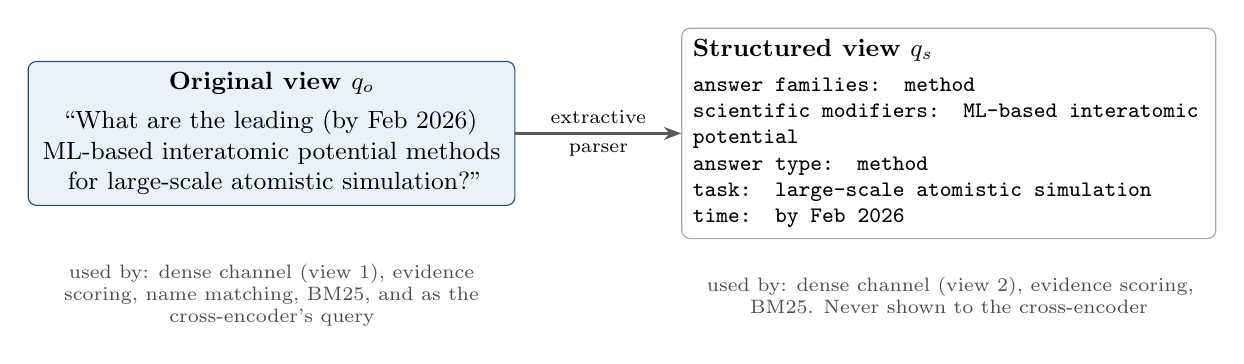
\begin{tikzpicture}[font=\small]
  \node[vbox,text width=5.9cm] (o) at (0,0) {\textbf{Original view $q_o$}\\[3pt]
    ``What are the leading (by Feb 2026) ML-based interatomic potential methods for
    large-scale atomistic simulation?''};
  \node[vplain,text width=6.5cm,align=flush left,font=\ttfamily\footnotesize] (s) at (8.6,0) {%
    {\normalfont\small\bfseries Structured view $q_s$}\\[3pt]
    answer families: method\\
    scientific modifiers: ML-based interatomic potential\\
    answer type: method\\
    task: large-scale atomistic simulation\\
    time: by Feb 2026};
  \draw[varr] (o.east) -- node[above,font=\scriptsize] {extractive} node[below,font=\scriptsize] {parser} (s.west);
  \node[font=\scriptsize,text=black!70,align=flush center,text width=5.9cm] at (0,-2.05)
    {used by: dense channel (view 1), evidence scoring, name matching, BM25, and as the
     cross-encoder's query};
  \node[font=\scriptsize,text=black!70,align=flush center,text width=6.5cm] at (8.6,-2.05)
    {used by: dense channel (view 2), evidence scoring, BM25. Never shown to the
     cross-encoder};
\end{tikzpicture}}
\caption[The two query views]{The two views of benchmark question Q12, exactly as stored in the frozen
\code{query\_understanding} trace. The structured view removes interrogative scaffolding
and isolates the task and modifiers; it contains only words copied from the question and
no candidate names. The original view is always preserved and is the only text the
cross-encoder sees as the query.}
\label{fig:views}
\end{figure}

The two views retrieve different things. The original view carries the full phrasing,
including conditions the parser may not separate. The structured view concentrates the
embedding on the task and its modifiers, which moves it toward task- and
technique-shaped evidence. Neither replaces the other: they feed separate dense lists,
and for evidence scoring an item takes the larger of its two similarities.

The parser is a heuristic. \Atag{} It can split a compound phrase imperfectly, and it
does not separate every modifier. That is acceptable only because the structured view is
\emph{supplementary}: the verbatim question is always present in parallel.

% ==================================================================
\section{First-Stage Candidate Generation}
\label{sec:channels}
% ==================================================================

Six ranked lists are produced for each question. Each list answers a different question
about a candidate, and each fails in a different way.

\subsection{Dense semantic retrieval}
\label{sec:dense}

\paragraph{Model.} \code{BAAI/bge-small-en-v1.5} \citep{xiao2023bge}, pinned at revision
\code{5c38ec7c405e} (full hash in \cref{tab:env}), run on CPU with weights loaded from
local files whose SHA-256 hashes are checked before prediction starts. It is a
\emph{bi-encoder} in the Sentence-BERT sense \citep{reimers2019sbert}: one transformer
maps any text to a single vector.

\paragraph{How it scores.} Every non-author node $v$ has a document: its own
``[type] surface form'' line followed by at most 12 deduplicated direct neighbours through
content relations, claims first. This is the main report's document builder, reused
unchanged. The encoder gives unit-norm vectors $\phi(\cdot)\in\R^{384}$, so cosine
similarity is an inner product. The score of an entity is the best score of its member
nodes:
\begin{equation}
  s_{\mathrm{d}}^{x}(e)=\max_{v\in\mathrm{nodes}(e)}\ \langle\phi(q_x),\phi(\mathrm{doc}(v))\rangle,
  \qquad x\in\{o,s\}.
\label{eq:dense}
\end{equation}
The two views give two separate lists; they are not averaged. The code passes each view
to the encoder as plain text and adds no instruction prefix of its own.

\begin{figure}[!htbp]
\centering
\fitfig{%
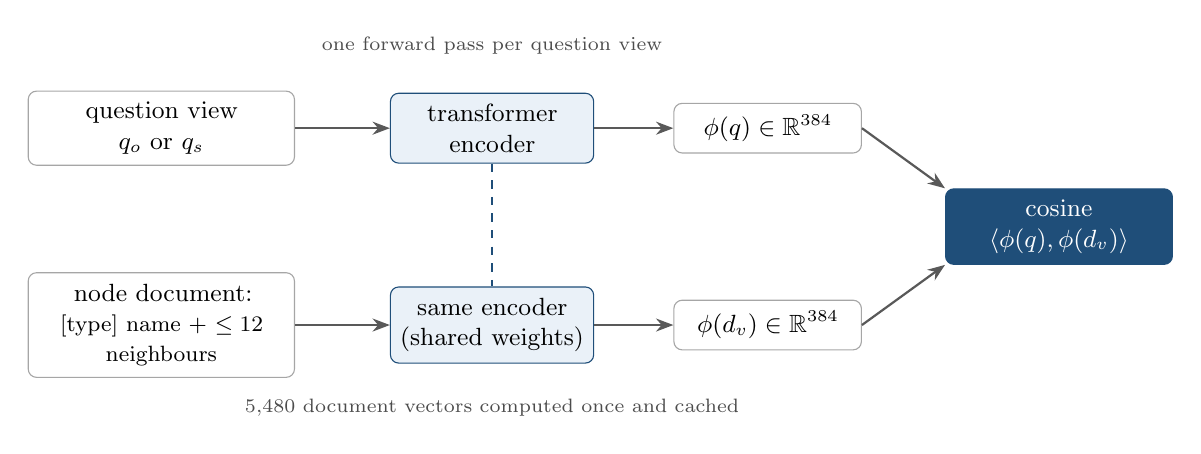
\begin{tikzpicture}[font=\small]
  \node[vplain,text width=3.1cm] (qt) at (0,1.25) {question view\\ $q_o$ or $q_s$};
  \node[vbox,text width=2.3cm] (e1) at (4.2,1.25) {transformer encoder};
  \node[vplain,text width=2.1cm] (qv) at (7.7,1.25) {$\phi(q)\in\R^{384}$};
  \node[vplain,text width=3.1cm] (dt) at (0,-1.25) {node document:\\ {\footnotesize [type] name + $\le12$ neighbours}};
  \node[vbox,text width=2.3cm] (e2) at (4.2,-1.25) {same encoder (shared weights)};
  \node[vplain,text width=2.1cm] (dv) at (7.7,-1.25) {$\phi(d_v)\in\R^{384}$};
  \node[vdark,text width=2.6cm] (cs) at (11.4,0) {cosine\\ $\langle\phi(q),\phi(d_v)\rangle$};
  \draw[varr] (qt) -- (e1); \draw[varr] (e1) -- (qv);
  \draw[varr] (dt) -- (e2); \draw[varr] (e2) -- (dv);
  \draw[varr] (qv.east) -- (cs.north west);
  \draw[varr] (dv.east) -- (cs.south west);
  \node[font=\scriptsize,text=black!70] at (4.2,-2.3) {5{,}480 document vectors computed once and cached};
  \node[font=\scriptsize,text=black!70] at (4.2,2.3) {one forward pass per question view};
  \draw[vlink] (e1) -- (e2);
\end{tikzpicture}}
\caption[Bi-encoder architecture of the dense channels]{The bi-encoder used by the dense and evidence channels. Question and document
pass through the same network \emph{separately}; each is compressed to one 384-dimensional
vector, and the only interaction between them is a final inner product. Because document
vectors do not depend on the question they are computed once, which makes scoring every
candidate cheap. The cost of that speed is that no question token ever attends to a
document token.}
\label{fig:biencoder}
\end{figure}

\paragraph{Why it is fast.} Document vectors are independent of the question. They are
encoded once and cached under a content hash; a question then costs one encoder pass per
view plus a matrix product.

\paragraph{Why it is imperfect.} All of a text's meaning must fit one vector, and the
question and the document never interact token by token. A short name carries little
signal, and a document whose \emph{context} resembles the question can outrank the entity
the question is about. This is the failure of \cref{fig:failure}, and the reason dense
retrieval is one channel among six rather than the retriever.

\subsection{BM25 lexical retrieval}
\label{sec:bm25}

BM25 \citep{robertson2009bm25} scores exact term overlap. Each entity gets one lexical
document: its names, its aliases and the text of every evidence item linked to it, each
item once. Text is case-folded and split into word tokens, keeping internal hyphens and
dots so that a token such as \code{e3-equivariant} survives intact. For a query $Q$ (the
original and the structured view concatenated) and entity document $d$:
\begin{equation}
  \mathrm{BM25}(Q,d)=\sum_{w\in Q}\ \underbrace{\ln\!\Bigl(1+\frac{N-n_w+0.5}{n_w+0.5}\Bigr)}_{\text{IDF}(w)}
  \cdot\frac{f_{w,d}\,(k_1+1)}{f_{w,d}+k_1\bigl(1-b+b\,|d|/\overline{|d|}\bigr)},
\label{eq:bm25}
\end{equation}
with $k_1=1.5$ and $b=0.75$ \Dtag. The three ingredients are:
\begin{itemize}
  \item \textbf{Term frequency} $f_{w,d}$: how often word $w$ occurs in $d$. The fraction
        saturates, so the tenth occurrence adds far less than the first; $k_1$ sets how
        quickly.
  \item \textbf{Inverse document frequency}: $n_w$ of the $N$ documents contain $w$. A word
        found in few documents is strong evidence; a word found everywhere is nearly
        worthless.
  \item \textbf{Length normalisation}: $|d|/\overline{|d|}$ compares the document's length
        with the average, so a long document is not favoured merely for containing more
        words; $b$ sets how strongly.
\end{itemize}
Each distinct query word is counted once, and an entity with no overlapping word gets no
entry at all, so it receives no vote in fusion. \Gtag

\paragraph{Toy example.} Take $N=1000$ entity documents and the query words
``equivariant'' ($n_w=20$) and ``potential'' ($n_w=600$). Then
$\mathrm{IDF}(\text{equivariant})=\ln(1+980.5/20.5)\approx3.89$ and
$\mathrm{IDF}(\text{potential})=\ln(1+400.5/600.5)\approx0.51$. For a document of average
length containing each word once, the second factor is $2.5/2.5=1$, so the rare technical
term contributes about 7.6 times as much as the common one. This is the behaviour one
wants for scientific text.

\paragraph{Why it complements dense retrieval.} An embedding smooths meaning; BM25 does
not. It is valuable precisely where smoothing hurts: technical terms, rare abbreviations,
exact terminology, names and aliases, and numbers or domain-specific tokens that a
general-purpose encoder may represent poorly. Conversely it is blind to paraphrase, which
the dense channels handle. \Atag{} (complementarity is a design premise; the measured
channel coverage is in \cref{tab:coverage}).

\subsection{Evidence-level dense retrieval}
\label{sec:evidence-channel}

This channel is the direct answer to \cref{fig:failure}. Instead of asking whether the
question resembles the entity's name,
\[
  \text{question}\ \longrightarrow\ \text{``MACE''},
\]
it asks whether the question resembles something the graph \emph{says about} the entity,
and then follows the link:
\[
  \text{question}\ \longrightarrow\ \text{relevant claim, task or other evidence}\ \longrightarrow\ \text{entity}.
\]

Each evidence item $i$ is embedded on its own, from its own text, with the same frozen
encoder. Its similarity to the question is the better of the two views:
\begin{equation}
  \simop_q(i)=\max\bigl(\langle\phi(q_o),\phi(i)\rangle,\ \langle\phi(q_s),\phi(i)\rangle\bigr).
\label{eq:evsim}
\end{equation}
Let $S_{500}(q)$ be the 500 items with the highest $\simop_q$ (the \emph{seeds}). An
entity inherits the score of its best linked seed:
\begin{equation}
  s_{\mathrm{ev}}(e)=\max_{\,i\in\Ev_t(e)\,\cap\,S_{500}(q)}\ \simop_q(i).
\label{eq:evidence}
\end{equation}
Entities owning no seed are absent from this list.

\begin{figure}[!htbp]
\centering
\fitfig{%
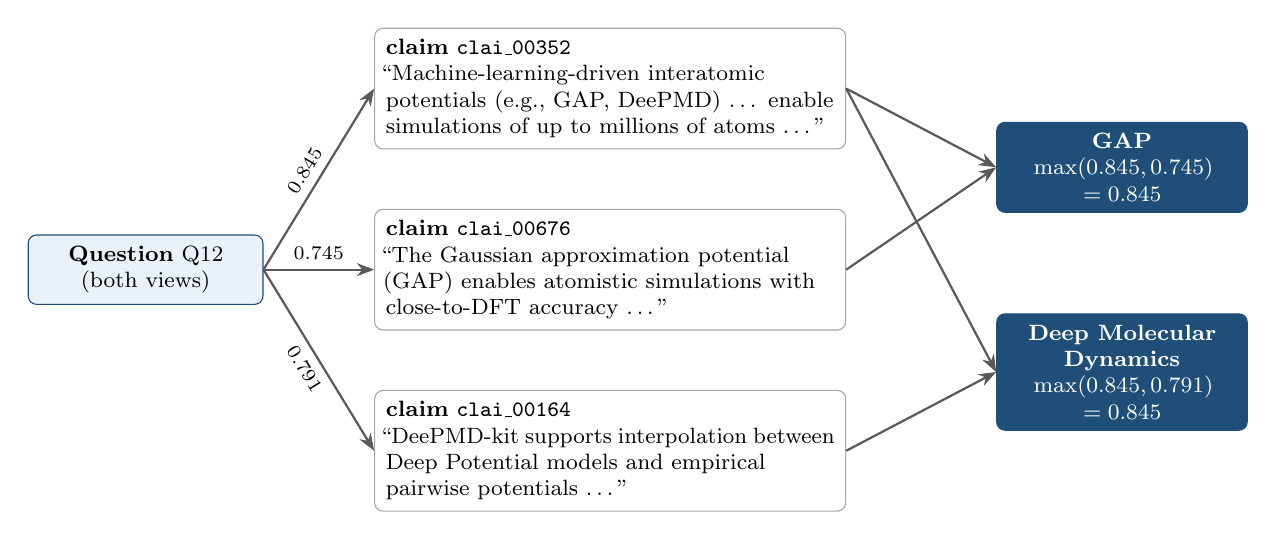
\begin{tikzpicture}[font=\footnotesize]
  \node[vbox,text width=2.7cm] (q) at (0,0) {\textbf{Question} Q12\\ (both views)};
  \node[vplain,text width=5.7cm,align=flush left] (i1) at (5.9,2.3) {\textbf{claim} \texttt{clai\_00352}\\
     ``Machine-learning-driven interatomic potentials (e.g., GAP, DeePMD) \dots\ enable
     simulations of up to millions of atoms \dots''};
  \node[vplain,text width=5.7cm,align=flush left] (i2) at (5.9,0) {\textbf{claim} \texttt{clai\_00676}\\
     ``The Gaussian approximation potential (GAP) enables atomistic simulations with
     close-to-DFT accuracy \dots''};
  \node[vplain,text width=5.7cm,align=flush left] (i3) at (5.9,-2.3) {\textbf{claim} \texttt{clai\_00164}\\
     ``DeePMD-kit supports interpolation between Deep Potential models and empirical
     pairwise potentials \dots''};
  \node[vdark,text width=2.9cm] (g) at (12.4,1.3) {\textbf{GAP}\\ $\max(0.845,0.745)$\\ $=0.845$};
  \node[vdark,text width=2.9cm] (d) at (12.4,-1.3) {\textbf{Deep Molecular Dynamics}\\ $\max(0.845,0.791)$\\ $=0.845$};
  \draw[varr] (q.east) -- node[above,sloped,font=\scriptsize] {0.845} (i1.west);
  \draw[varr] (q.east) -- node[above,font=\scriptsize] {0.745} (i2.west);
  \draw[varr] (q.east) -- node[below,sloped,font=\scriptsize] {0.791} (i3.west);
  \draw[varr] (i1.east) -- (g.west);
  \draw[varr] (i2.east) -- (g.west);
  \draw[varr] (i1.east) -- (d.west);
  \draw[varr] (i3.east) -- (d.west);
\end{tikzpicture}}
\caption[Evidence-to-entity retrieval]{Evidence-to-entity retrieval, with similarities and links read from the frozen
trace of question Q12. Each claim is embedded independently and compared with the
question. A claim then passes its similarity to every entity it is linked to; here the
links are safe literal mentions of the entity's name or graph alias. One claim can
support several entities, and an entity keeps the maximum over its linked seeds. The
long, question-like claims that would have outranked a bare method name now vote for it.
(Each entity has further seeds, omitted for clarity; the maximum shown is the logged
channel score.)}
\label{fig:evidence}
\end{figure}

\paragraph{Why max pooling.} The alternatives are a sum or a mean over an entity's
evidence. A sum rewards entities for having \emph{many} linked items, which favours
heavily cited or heavily described entities regardless of the question. A mean punishes an
entity for also having evidence about unrelated matters. The maximum asks the question
that matters for admission: is there \emph{at least one} piece of evidence strongly
related to the question? It is also invariant to how much unrelated evidence an entity
carries. \Dtag

\subsection{Safe name and alias channel}
\label{sec:name-channel}

This channel has a narrow purpose: if a question literally names an entity, that entity
should be admitted. An entity enters the list when one of its names or graph aliases
occurs in the original question as a whole token sequence, and only if the name is
\emph{safe}: at least three characters long and either identifier-like (it contains a
digit, a lower-case letter followed by an upper-case one, or is entirely upper case) or
multi-word with at least ten characters. The score is the length of the longest match.
The rule exists to stop short generic words from matching.

Its contribution should not be overstated. Benchmark questions describe a need; they do
not name their answers. In the frozen run this list is empty for 9 of 18 questions and
never longer than two entities, and it contains none of the 49 mapped targets. \Mtag{}
What it matched were terms the question uses in passing, such as ``DFT''. The same safe
rule also decides which claims count as literal mentions (\cref{sec:evidence-links}),
and it is conservative: ``CHGNet'', ``MEGNet'' and ``Orb'' are not identifier-like under
it, so those entities receive no mention evidence. \Mtag

\subsection{Bounded graph expansion}
\label{sec:graph-channel}

The last channel uses structure. Starting from the 200 most question-similar evidence
items, it follows directed, role-checked arcs to eligible entities. Only the path shapes
of \cref{fig:paths} exist.

\begin{figure}[H]
\centering
\fitfig{%
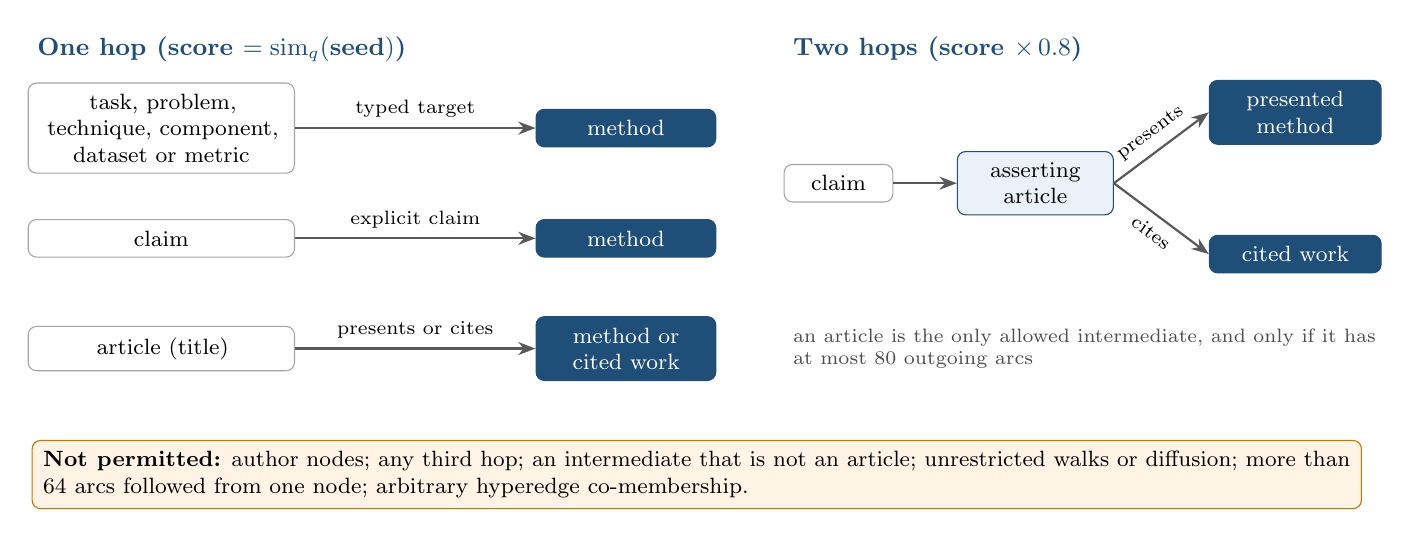
\begin{tikzpicture}[font=\footnotesize]
  % one hop
  \node[font=\small\bfseries,text=accent,anchor=west] at (-1.5,3.5) {One hop (score $=\simop_q(\text{seed})$)};
  \node[vplain,text width=3.1cm] (a1) at (0.2,2.5) {task, problem, technique, component, dataset or metric};
  \node[vdark,text width=2.0cm] (a2) at (6.1,2.5) {method};
  \draw[varr] (a1) -- node[above,font=\scriptsize] {typed target} (a2);
  \node[vplain,text width=3.1cm] (b1) at (0.2,1.1) {claim};
  \node[vdark,text width=2.0cm] (b2) at (6.1,1.1) {method};
  \draw[varr] (b1) -- node[above,font=\scriptsize] {explicit claim} (b2);
  \node[vplain,text width=3.1cm] (c1) at (0.2,-0.3) {article (title)};
  \node[vdark,text width=2.0cm] (c2) at (6.1,-0.3) {method or cited work};
  \draw[varr] (c1) -- node[above,font=\scriptsize] {presents or cites} (c2);
  % two hops
  \node[font=\small\bfseries,text=accent,anchor=west] at (8.1,3.5) {Two hops (score $\times\,0.8$)};
  \node[vplain,text width=1.1cm] (d1) at (8.8,1.8) {claim};
  \node[vbox,text width=1.7cm] (d2) at (11.3,1.8) {asserting article};
  \node[vdark,text width=1.9cm] (d3) at (14.6,2.7) {presented method};
  \node[vdark,text width=1.9cm] (d4) at (14.6,0.9) {cited work};
  \draw[varr] (d1) -- (d2);
  \draw[varr] (d2.east) -- node[above,sloped,font=\scriptsize] {presents} (d3.west);
  \draw[varr] (d2.east) -- node[below,sloped,font=\scriptsize] {cites} (d4.west);
  \node[font=\scriptsize,text=black!70,align=flush left,anchor=west,text width=7.4cm] at (8.1,-0.3)
    {an article is the only allowed intermediate, and only if it has at most 80 outgoing arcs};
  % forbidden
  \node[vwarn,text width=16.6cm,align=flush left] at (7.0,-1.9) {\textbf{Not permitted:} author nodes; any
     third hop; an intermediate that is not an article; unrestricted walks or diffusion;
     more than 64 arcs followed from one node; arbitrary hyperedge co-membership.};
\end{tikzpicture}}
\caption[Permitted graph expansion paths]{Every path shape the graph channel can follow, from the implementation. A seed is
an evidence item similar to the question; arrows are directed arcs created only from
hyperedges whose members fit the relation's role pattern. A path's score is the seed's
similarity multiplied by 0.8 for each hop beyond the first, and an entity keeps its best
path. Depth, fan-out and hub size are all capped, and authors are never traversed. Each
retained path stores its hyperedge ids, relations, years and provenance.}
\label{fig:paths}
\end{figure}

\begin{algorithm}[!htbp]
\caption{Bounded graph expansion}
\label{alg:graph}
\begin{algorithmic}[1]
\Require Seeds $(i,\simop_q(i))$ sorted by similarity; arcs; eligible set $\Ent_t(q)$
\Ensure Graph score $s_{\mathrm{gr}}(e)$ and up to 8 provenance paths per entity
\For{each of the first 200 seeds $i$}
  \For{each of the first 64 arcs $i\to x$}
    \State paths $\gets\{(i\to x)\}$
    \If{$x$ is an article with at most 80 outgoing arcs}
      \State add $(i\to x\to y)$ for each of the first 64 arcs $x\to y$ with relation
             \code{presents} or \code{cites}, $y\neq i$
    \EndIf
    \For{each path $p$ ending at node $z$ of an eligible entity $e$}
      \State $s_{\mathrm{gr}}(e)\gets\max\bigl(s_{\mathrm{gr}}(e),\ \simop_q(i)\cdot0.8^{|p|-1}\bigr)$
      \State record $p$ with its hyperedge ids, relations, years and provenance
    \EndFor
  \EndFor
\EndFor
\State keep the 8 best paths per entity, ties broken by seed id
\end{algorithmic}
\end{algorithm}

\paragraph{What it adds.} An entity can be relevant without any evidence item of its own
resembling the question. If a paper whose title or claims match the question
\emph{presents} or \emph{cites} the entity, the graph channel can still admit it.
For example, in the frozen Q12 trace the cited-work entity GAP is reached in one hop from
a review article's title (similarity 0.826, so score 0.826) and in two hops from a claim
about DeePMD-kit through that claim's article (similarity 0.791, so score
$0.791\times0.8=0.633$). \Mtag

\begin{cautionbox}[Structural context is not entailment]
A path says that an entity is \emph{near} question-relevant text in the graph. It does
not say that the text is \emph{about} the entity, and still less that the entity
satisfies the question. The two-hop example above reaches GAP from a claim about a
different method. Across all retained paths of the frozen run, 18{,}230 of 22{,}122
(82\%) pass through a citation arc. \Mtag{} The implementation labels every such path
\code{structural\_path\_not\_entailment} and carries that label into the evidence card.
The graph channel is an admission signal only.
\end{cautionbox}

\subsection{Summary and measured coverage}

\Cref{tab:channels} summarises the six lists. \Cref{tab:coverage} then reports, for the
frozen run, how many of the directly mapped targets each list reaches when used alone.

\begin{table}[!htbp]
\centering
\caption[The six first-stage lists]{The six first-stage lists. Each is truncated to 500 entities before fusion.}
\label{tab:channels}
\small
\begin{tabularx}{\linewidth}{p{2.7cm}p{4.3cm}X}
\toprule
List & Score & What it can find; how it fails\\
\midrule
Dense, original & \cref{eq:dense} with $q_o$ & Paraphrase of the full question; misled by
  short names and by context\\
Dense, structured & \cref{eq:dense} with $q_s$ & Task- and modifier-focused paraphrase;
  inherits parser errors\\
BM25 & \cref{eq:bm25} & Exact technical terms, names, aliases; blind to paraphrase\\
Safe name & length of longest match & An entity literally named in the question; usually
  empty\\
Evidence owner & \cref{eq:evidence} & Entities whose linked evidence matches the question;
  needs evidence to exist\\
Bounded graph & best path score & Entities presented or cited near matching text;
  structural, not semantic\\
\bottomrule
\end{tabularx}
\end{table}

\begin{table}[!htbp]
\centering
\caption[Measured coverage of mapped targets per list]{Coverage of the 49 directly mapped target occurrences by each list alone, within
its 500-entity truncation. \Mtag{} ``Unique'' counts targets found by that list and by no
other. Source: \code{channel\_diagnostics} in the frozen \code{metrics.json}.}
\label{tab:coverage}
\small
\begin{tabular}{lrrr}
\toprule
List & Targets covered & Fraction of 49 & Unique\\
\midrule
Dense, original view & 19 & 0.388 & 0\\
Dense, structured view & 21 & 0.429 & 0\\
BM25 & 41 & 0.837 & 0\\
Safe name & 0 & 0.000 & 0\\
Evidence owner & 44 & 0.898 & 0\\
Bounded graph & 37 & 0.755 & 1\\
\midrule
Union of all six & 46 & 0.939 & \\
\bottomrule
\end{tabular}
\end{table}

\Cref{tab:coverage} supports the design argument of \cref{fig:failure} on this benchmark:
the two dense lists, which compare the question with the entity's own document, cover
fewer than half of the mapped targets, while the evidence-owner list covers 44 of 49.
\Otag{} The three targets no list covers are the three removed by the answer-family filter
(\cref{sec:family}).

% ==================================================================
\section{Multi-Channel Union and Rank Fusion}
\label{sec:rrf}
% ==================================================================

\begin{figure}[!htbp]
\centering
\fitfig{%
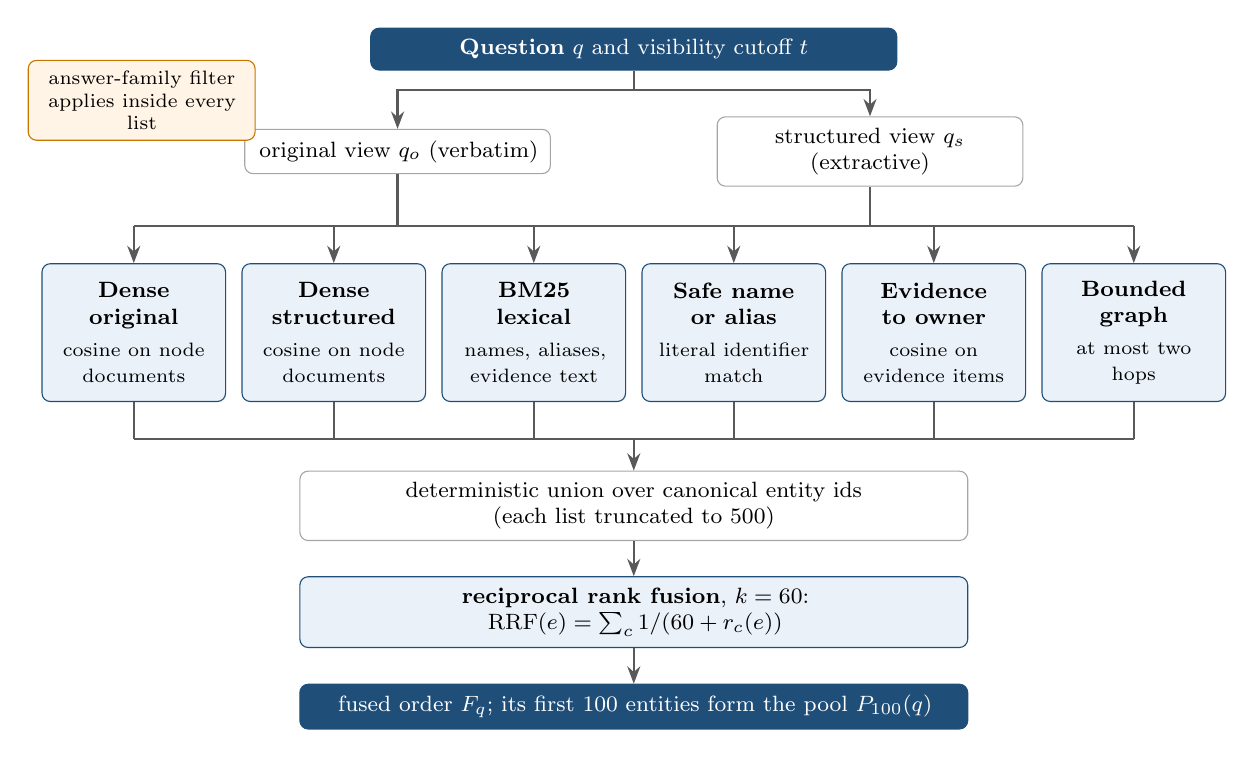
\begin{tikzpicture}[font=\footnotesize]
  \node[vdark,text width=6.4cm] (q) at (7.6,0.3) {\textbf{Question} $q$ and visibility cutoff $t$};
  \node[vplain,text width=3.6cm] (qo) at (4.6,-1.0) {original view $q_o$ (verbatim)};
  \node[vplain,text width=3.6cm] (qs) at (10.6,-1.0) {structured view $q_s$ (extractive)};
  \draw[varr] (q.south) -- ++(0,-0.25) -| (qo.north);
  \draw[varr] (q.south) -- ++(0,-0.25) -| (qs.north);
  \draw[vline] (qo.south) -- (4.6,-1.95);
  \draw[vline] (qs.south) -- (10.6,-1.95);
  \draw[vline] (1.25,-1.95) -- (13.95,-1.95);
  \foreach \x/\nm/\la/\lb/\sub in {
     1.25/c1/Dense/original/{cosine on node documents},
     3.79/c2/Dense/structured/{cosine on node documents},
     6.33/c3/BM25/lexical/{names, aliases, evidence text},
     8.87/c4/Safe name/or alias/{literal identifier match},
     11.41/c5/Evidence/to owner/{cosine on evidence items},
     13.95/c6/Bounded/graph/{at most two hops}}{
    \node[vbox,text width=2.05cm,minimum height=1.75cm] (\nm) at (\x,-3.3) {\textbf{\la}\\ \textbf{\lb}\\[2pt]{\scriptsize \sub}};
    \draw[varr] (\x,-1.95) -- (\nm.north);
    \draw[vline] (\nm.south) -- (\x,-4.65);
  }
  \draw[vline] (1.25,-4.65) -- (13.95,-4.65);
  \node[vplain,text width=8.2cm] (u) at (7.6,-5.5) {deterministic union over canonical entity ids\\ (each list truncated to 500)};
  \node[vbox,text width=8.2cm] (r) at (7.6,-6.85) {\textbf{reciprocal rank fusion}, $k=60$:\quad $\RRF(e)=\sum_c 1/(60+r_c(e))$};
  \node[vdark,text width=8.2cm] (p) at (7.6,-8.05) {fused order $F_q$; its first 100 entities form the pool $P_{100}(q)$};
  \draw[varr] (7.6,-4.65) -- (u.north);
  \draw[varr] (u) -- (r); \draw[varr] (r) -- (p);
  \node[vwarn,text width=2.6cm,font=\scriptsize] at (1.35,-0.35) {answer-family filter applies inside every list};
\end{tikzpicture}}
\caption[Multi-channel first-stage architecture]{The first stage. One question becomes two views; six lists are computed
independently, each restricted to eligible entities; their union is ordered by reciprocal
rank fusion. Nothing in this stage is learned and nothing depends on run order: lists are
sorted by score with ties broken by entity id, and the fusion sums are accumulated in a
fixed channel order.}
\label{fig:architecture}
\end{figure}

\subsection{Reciprocal rank fusion}

The six lists must be combined into one order. V2 uses reciprocal rank fusion
\citep{cormack2009rrf}:

\begin{definition}[RRF score]
\label{def:rrf}
Let $r_c(e)\in\{1,2,\dots\}$ be the rank of entity $e$ in list $c$. Then
\begin{equation}
  \RRF(e)=\sum_{c\,:\,e\in L_c}\frac{1}{k+r_c(e)},\qquad k=60,
\label{eq:rrf}
\end{equation}
where a list that does not contain $e$ contributes nothing. Entities are sorted by
decreasing $\RRF$, ties broken by entity id.
\end{definition}

The constant $k$ controls how much the very top of a list dominates. With $k=60$, rank 1
contributes $1/61$ and rank 10 contributes $1/70$: close enough that agreement between
several lists outweighs a single first place. $k=60$ is the value proposed in the
original paper and was fixed in advance. \Dtag

\begin{figure}[!htbp]
\centering
\fitfig{%
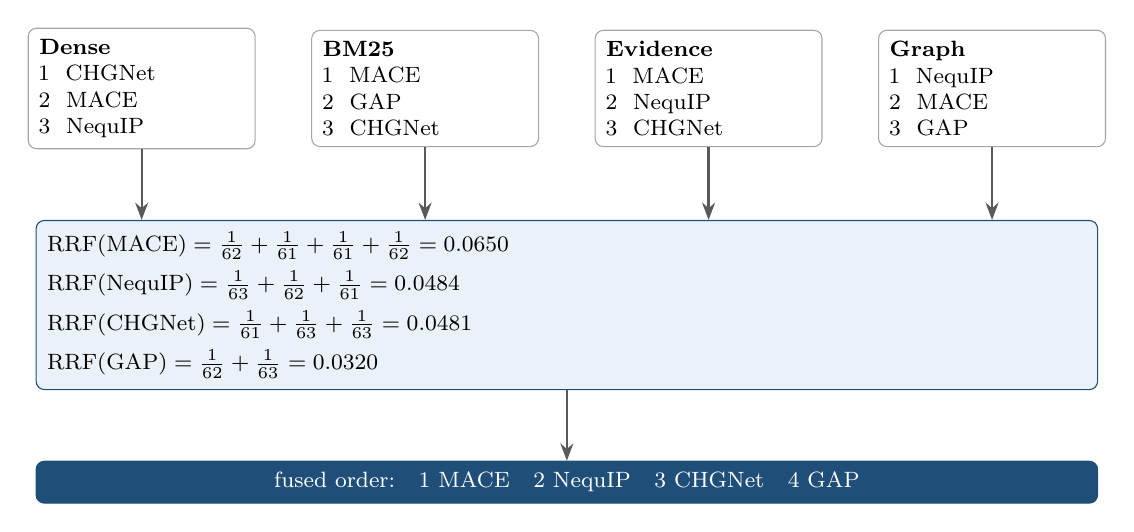
\begin{tikzpicture}[font=\footnotesize]
  \node[vplain,text width=2.6cm,align=flush left] (l1) at (0,0) {\textbf{Dense}\\ 1\ \ CHGNet\\ 2\ \ MACE\\ 3\ \ NequIP};
  \node[vplain,text width=2.6cm,align=flush left] (l2) at (3.6,0) {\textbf{BM25}\\ 1\ \ MACE\\ 2\ \ GAP\\ 3\ \ CHGNet};
  \node[vplain,text width=2.6cm,align=flush left] (l3) at (7.2,0) {\textbf{Evidence}\\ 1\ \ MACE\\ 2\ \ NequIP\\ 3\ \ CHGNet};
  \node[vplain,text width=2.6cm,align=flush left] (l4) at (10.8,0) {\textbf{Graph}\\ 1\ \ NequIP\\ 2\ \ MACE\\ 3\ \ GAP};
  \node[vbox,text width=13.2cm,align=flush left] (f) at (5.4,-2.75) {%
     $\RRF(\text{MACE})=\frac{1}{62}+\frac{1}{61}+\frac{1}{61}+\frac{1}{62}=0.0650$\\[3pt]
     $\RRF(\text{NequIP})=\frac{1}{63}+\frac{1}{62}+\frac{1}{61}=0.0484$\\[3pt]
     $\RRF(\text{CHGNet})=\frac{1}{61}+\frac{1}{63}+\frac{1}{63}=0.0481$\\[3pt]
     $\RRF(\text{GAP})=\frac{1}{62}+\frac{1}{63}=0.0320$};
  \node[vdark,text width=13.2cm] (o) at (5.4,-5.0) {fused order:\quad 1 MACE\quad 2 NequIP\quad 3 CHGNet\quad 4 GAP};
  \foreach \n in {l1,l2,l3,l4}{\draw[varr] (\n.south) -- (\n.south|-f.north);}
  \draw[varr] (f) -- (o);
\end{tikzpicture}}
\caption[Toy reciprocal rank fusion example]{A toy fusion with four \emph{fictional} rankings, constructed for teaching and
not taken from any run. MACE is first in only two lists but present near the top of all
four, so it wins clearly. NequIP and CHGNet each appear in three lists; NequIP edges ahead
because its ranks (3, 2, 1) are slightly better than CHGNet's (1, 3, 3). GAP appears in
only two lists and comes last. Only ranks enter the computation; no raw score appears
anywhere.}
\label{fig:rrf}
\end{figure}

\begin{keybox}[RRF solves a calibration problem]
The channels' raw scores live on unrelated scales. In the frozen Q12 trace the best dense
cosine is 0.835, the best BM25 score is 18.61, the single name score is 32, and graph
scores are cosines multiplied by a decay. \Mtag{} Adding them would let BM25 or the name
length dominate for no scientific reason; rescaling them would require weights, and
weights would have to be fitted on the very benchmark being evaluated. A rank is
comparable across channels without any fitting.
\end{keybox}

Rank fusion has costs. It discards magnitude: a channel that is very confident and one
that barely prefers its top result contribute equally. And it rewards agreement, so an
entity found by one channel at rank 1 can be placed below an entity that several channels
rank at 40. Both effects are visible in the worked example of \cref{sec:worked}.

% ==================================================================
\section{Candidate Admission versus Ranking}
\label{sec:two-stage}
% ==================================================================

\begin{figure}[!htbp]
\centering
\fitfig{%
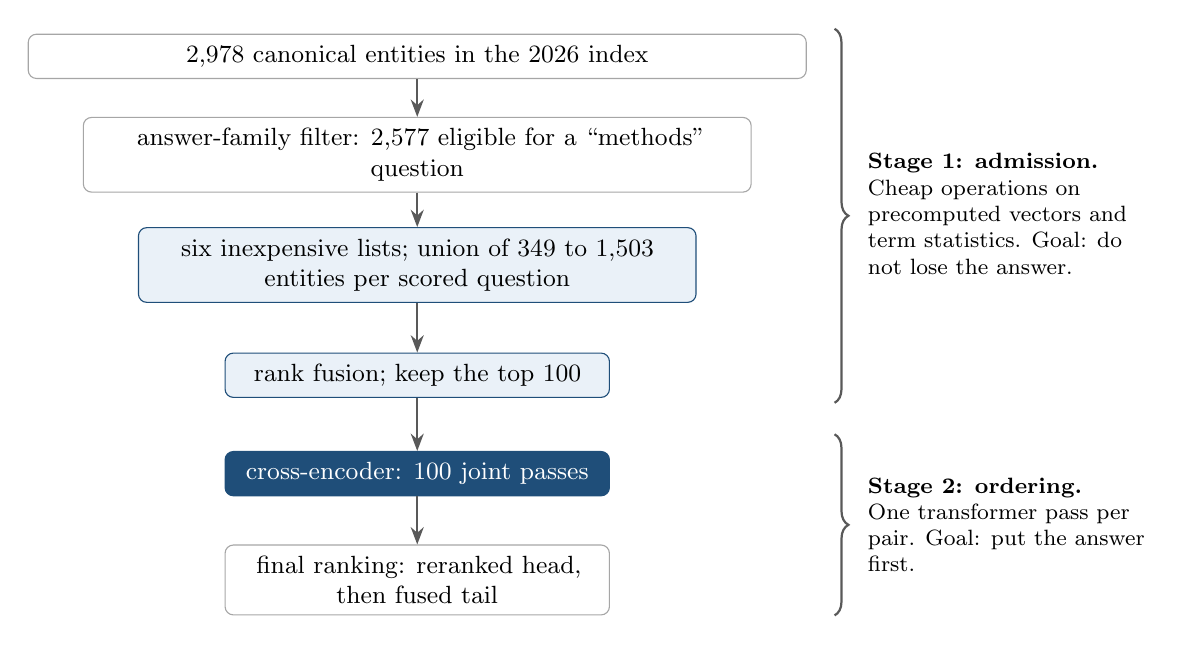
\begin{tikzpicture}[font=\small]
  \node[vplain,text width=9.6cm] (a) at (0,0) {2{,}978 canonical entities in the 2026 index};
  \node[vplain,text width=8.2cm] (b) at (0,-1.25) {answer-family filter: 2{,}577 eligible for a ``methods'' question};
  \node[vbox,text width=6.8cm] (c) at (0,-2.65) {six inexpensive lists; union of 349 to 1{,}503 entities per scored question};
  \node[vbox,text width=4.6cm] (d) at (0,-4.05) {rank fusion; keep the top 100};
  \node[vdark,text width=4.6cm] (e) at (0,-5.3) {cross-encoder: 100 joint passes};
  \node[vplain,text width=4.6cm] (f) at (0,-6.65) {final ranking: reranked head, then fused tail};
  \draw[varr] (a)--(b); \draw[varr] (b)--(c); \draw[varr] (c)--(d); \draw[varr] (d)--(e); \draw[varr] (e)--(f);
  \draw[decorate,decoration={brace,amplitude=5pt},thick,gray!70!black] (5.3,0.35) -- (5.3,-4.4);
  \node[anchor=west,text width=3.6cm,align=flush left,font=\footnotesize] at (5.6,-2.0)
     {\textbf{Stage 1: admission.}\\ Cheap operations on precomputed vectors and term
      statistics. Goal: do not lose the answer.};
  \draw[decorate,decoration={brace,amplitude=5pt},thick,gray!70!black] (5.3,-4.8) -- (5.3,-7.1);
  \node[anchor=west,text width=3.6cm,align=flush left,font=\footnotesize] at (5.6,-5.95)
     {\textbf{Stage 2: ordering.}\\ One transformer pass per pair. Goal: put the answer
      first.};
\end{tikzpicture}}
\caption[Two-stage funnel: admission and ordering]{The two-stage funnel with counts from the frozen run. Stage one applies cheap
operations to every eligible entity and is judged by recall. Stage two applies an
expensive joint model to 100 candidates and is judged by ordering quality. Entities
ranked below 100 by fusion are not discarded: they keep their fused order after the
reranked head.}
\label{fig:funnel}
\end{figure}

The split is first a matter of cost. A bi-encoder comparison is an inner product of two
vectors that already exist. A cross-encoder comparison is a full transformer forward pass
over the concatenated question and candidate text, and it cannot be precomputed because
its input depends on the question. Running it over all 2{,}577 eligible entities would
cost about 26 times as many forward passes per question as running it over 100. The two
stages therefore optimise different things:

\begin{itemize}
  \item \textbf{First stage: maximise reasonable recall.} False positives are tolerable,
        because the next stage will reorder them. False negatives are permanent
        (\cref{prop:ceiling}).
  \item \textbf{Second stage: maximise ordering quality.} It may spend a model's full
        capacity on each pair, because there are few pairs.
\end{itemize}

The pool size $K$ trades admission against the amount of plausible-but-wrong material the
reranker must sort through.

\begin{cautionbox}[How $K=100$ was chosen]
\label{sec:k-status}
Among the predeclared reranking depths evaluated during development, $K=100$ gave the
strongest observed top-10 recovery. This supplement describes that simplified
configuration. This selection was made after development results were available and is
therefore a development choice, not an independently validated optimum. \Otag{} The
original frozen run declared a deeper pool as its primary setting; $K=100$ was one of
its predeclared alternatives, not its primary configuration.
\end{cautionbox}

% ==================================================================
\section{Cross-Encoder Reranking: the A6 Stage}
\label{sec:crossencoder}
% ==================================================================

What distinguishes A6 from its own first stage is one additional operation: the first 100
fused candidates are rescored by a model that reads the question and the candidate
\emph{together}.

\subsection{Bi-encoder and cross-encoder}

\begin{figure}[!htbp]
\centering
\fitfig{%
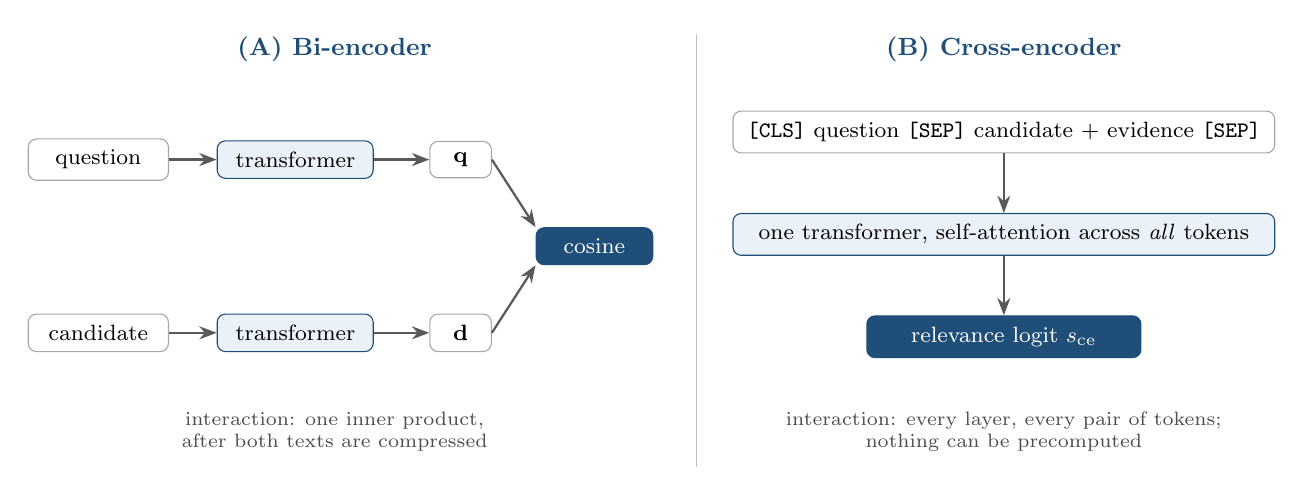
\begin{tikzpicture}[font=\footnotesize]
  % panel A
  \node[font=\small\bfseries,text=accent] at (3.0,2.5) {(A) Bi-encoder};
  \node[vplain,text width=1.5cm] (aq) at (0,1.1) {question};
  \node[vbox,text width=1.7cm] (at) at (2.5,1.1) {transformer};
  \node[vplain,text width=0.5cm] (av) at (4.6,1.1) {$\mathbf q$};
  \node[vplain,text width=1.5cm] (ad) at (0,-1.1) {candidate};
  \node[vbox,text width=1.7cm] (au) at (2.5,-1.1) {transformer};
  \node[vplain,text width=0.5cm] (aw) at (4.6,-1.1) {$\mathbf d$};
  \node[vdark,text width=1.2cm] (ac) at (6.3,0) {cosine};
  \draw[varr] (aq)--(at); \draw[varr] (at)--(av); \draw[varr] (ad)--(au); \draw[varr] (au)--(aw);
  \draw[varr] (av.east) -- (ac.north west); \draw[varr] (aw.east) -- (ac.south west);
  \node[font=\scriptsize,text=black!70,align=flush center] at (3.0,-2.35) {interaction: one inner product,\\ after both texts are compressed};
  % divider
  \draw[gray!50] (7.6,2.7) -- (7.6,-2.8);
  % panel B
  \node[font=\small\bfseries,text=accent] at (11.5,2.5) {(B) Cross-encoder};
  \node[vplain,text width=6.6cm] (bi) at (11.5,1.45) {\texttt{[CLS]} question \texttt{[SEP]} candidate + evidence \texttt{[SEP]}};
  \node[vbox,text width=6.6cm] (bt) at (11.5,0.15) {one transformer, self-attention across \emph{all} tokens};
  \node[vdark,text width=3.2cm] (bo) at (11.5,-1.15) {relevance logit $s_{\mathrm{ce}}$};
  \draw[varr] (bi)--(bt); \draw[varr] (bt)--(bo);
  \node[font=\scriptsize,text=black!70,align=flush center] at (11.5,-2.35) {interaction: every layer, every pair of tokens;\\ nothing can be precomputed};
\end{tikzpicture}}
\caption[Bi-encoder versus cross-encoder]{The two ways of scoring a question--candidate pair. (A) A bi-encoder encodes the
two texts separately and compares two fixed vectors. (B) A cross-encoder concatenates the
texts and lets every token attend to every other token before producing a single score.
(A) is cheap and used to search everything; (B) is expensive and used on 100 candidates.}
\label{fig:bi-vs-cross}
\end{figure}

In a transformer layer \citep{vaswani2017attention} each token's new representation is a
weighted mixture of all tokens in the sequence:
\begin{equation}
  h_i^{(\ell+1)}=g\Bigl(h_i^{(\ell)},\ \sum_{j}\alpha_{ij}^{(\ell)}\,h_j^{(\ell)}\Bigr),\qquad
  \alpha_{ij}^{(\ell)}=\operatorname{softmax}_j\bigl(\langle W_Qh_i^{(\ell)},W_Kh_j^{(\ell)}\rangle/\sqrt{d}\bigr).
\end{equation}
In a bi-encoder the sum runs over the tokens of \emph{one} text. In a cross-encoder it
runs over the concatenation, so the attention weight $\alpha_{ij}$ can connect a question
token $i$ to a candidate token $j$ in every layer \citep{devlin2019bert,nogueira2019passage}.
The model can therefore check whether a specific condition in the question is addressed by
a specific phrase in the candidate's evidence, which a single pooled vector cannot
represent reliably.

\begin{figure}[!htbp]
\centering
\fitfig{%
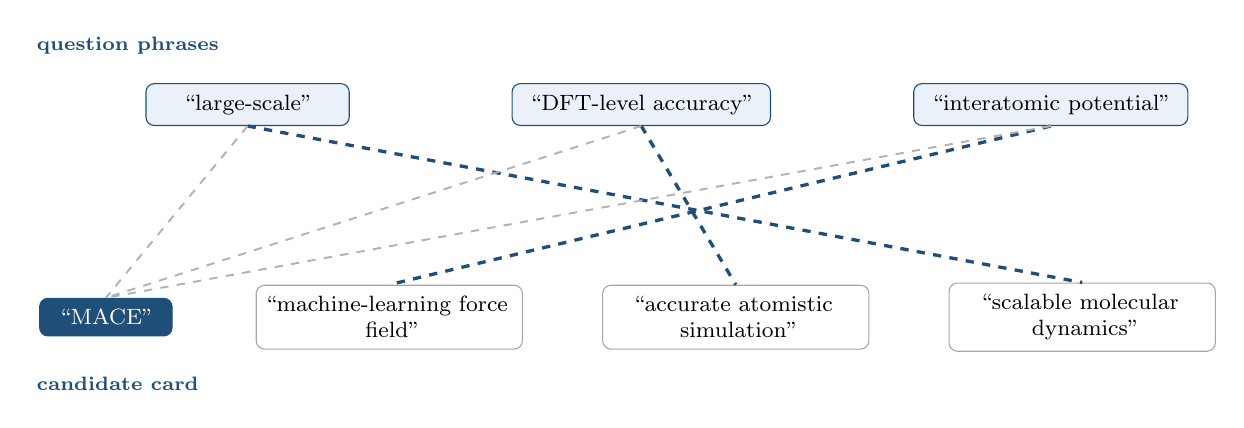
\begin{tikzpicture}[font=\footnotesize]
  \node[font=\scriptsize\bfseries,text=accent,anchor=west] at (-1.4,3.45) {question phrases};
  \node[font=\scriptsize\bfseries,text=accent,anchor=west] at (-1.4,-0.85) {candidate card};
  \node[vbox,text width=2.3cm] (q1) at (1.4,2.7) {``large-scale''};
  \node[vbox,text width=3.0cm] (q2) at (6.4,2.7) {``DFT-level accuracy''};
  \node[vbox,text width=3.2cm] (q3) at (11.6,2.7) {``interatomic potential''};
  \node[vdark,text width=1.4cm] (c0) at (-0.4,0) {``MACE''};
  \node[vplain,text width=3.1cm] (c1) at (3.2,0) {``machine-learning force field''};
  \node[vplain,text width=3.1cm] (c2) at (7.6,0) {``accurate atomistic simulation''};
  \node[vplain,text width=3.1cm] (c3) at (12.0,0) {``scalable molecular dynamics''};
  \draw[vlink,line width=1.2pt] (q1.south) -- (c3.north);
  \draw[vlink,line width=1.2pt] (q2.south) -- (c2.north);
  \draw[vlink,line width=1.2pt] (q3.south) -- (c1.north);
  \draw[vlink,gray!60] (q1.south) -- (c0.north);
  \draw[vlink,gray!60] (q2.south) -- (c0.north);
  \draw[vlink,gray!60] (q3.south) -- (c0.north);
\end{tikzpicture}}
\caption[Joint attention between question and candidate phrases]{What joint attention makes possible, as a schematic. The question's conditions
(top) can be matched with the corresponding phrases in the candidate's evidence (bottom):
``large-scale'' with ``scalable molecular dynamics'', ``DFT-level accuracy'' with ``accurate
atomistic simulation'', ``interatomic potential'' with ``machine-learning force field''.
All of them connect to the identity ``MACE'', which by itself shares no words with the
question. The phrases and links are illustrative; attention weights were not measured.}
\label{fig:attention}
\end{figure}

\subsection{The model actually used}

The reranker is \code{cross-encoder/ms-marco-MiniLM-L6-v2}, pinned at revision
\code{233902d25c44} (full hash in \cref{tab:env}), loaded from local files with hash
checks and run on CPU. It is a MiniLM-family transformer \citep{wang2020minilm} with a single
regression output, trained for passage relevance on MS~MARCO web-search data
\citep{bajaj2016msmarco}. Its use here follows the standard retrieve-then-rerank pattern
\citep{nogueira2019passage}.

\begin{keybox}[Why a cross-encoder?]
Unlike a bi-encoder, query and candidate tokens interact in the same transformer. The
question's wording can be matched against the candidate's evidence phrase by phrase,
instead of comparing two summaries.
\end{keybox}

\begin{cautionbox}[What the output is and is not]
The model's output is a \textbf{relevance logit}: an unbounded real number whose only
meaningful use here is to order candidates of the same question. It is \emph{not} an
entailment or NLI judgement, \emph{not} a statement of scientific truth, and \emph{not} a
calibrated probability. No sigmoid, threshold or cross-question comparison is applied.
The loader refuses any model that has more than one output or NLI-style labels. \Gtag
\end{cautionbox}

\subsection{The ranking rule}

For each $e\in P_{100}(q)$ the model receives the original question $q_o$ and the packed
candidate card $\mathrm{card}(e,q)$ of \cref{sec:card} and returns
$s_{\mathrm{ce}}(q,e)\in\R$. The final ranking is
\begin{equation}
  \pi_q=\underbrace{\operatorname{sort}\bigl(P_{100}(q);\ -s_{\mathrm{ce}},\ \text{entity id}\bigr)}_{\text{reranked head}}
  \ \oplus\ \underbrace{F_q[101{:}]}_{\text{untouched fused tail}} .
\label{eq:final}
\end{equation}
The head is ordered by logit alone; the fused score is not mixed back in. The tail is
exactly the fused order, so every entity of the union keeps a final rank. \Gtag{} The
test \path{test_reranker_only_changes_frozen_prefix} checks this.

% ==================================================================
\section{The Query-Dependent Candidate Card}
\label{sec:card}
% ==================================================================

A cross-encoder judges text. Given only ``MACE'', it would face the problem of
\cref{fig:failure} again. So each candidate is presented as a \emph{card}: its identity
followed by a bounded selection of its most question-relevant evidence.

\subsection{What the card contains}

The identity block is always first:
\begin{center}
\code{Candidate: <name>}\quad\code{Type: <member types>}
\end{center}
It is followed by evidence blocks drawn from ten families, visited in the fixed priority
order of \cref{tab:caps}. Within a family, rows are sorted by decreasing question
similarity $\simop_q$ of \cref{eq:evsim}, then candidate-specific rows before contextual
ones, then by evidence id. Each block is rendered as
\code{<family> [<support kind>]: <evidence text>}, so the model sees how the evidence is
connected to the candidate.

\begin{table}[!htbp]
\centering
\caption[Evidence families and caps of the candidate card]{Evidence families of the card, in priority order, with the maximum number of
blocks per family from \code{config.json}. \Dtag{} At most 20 evidence blocks follow the
identity.}
\label{tab:caps}
\small
\begin{tabularx}{\linewidth}{rlrX}
\toprule
 & Family & Cap & How the evidence is attached to the candidate\\
\midrule
1 & claims & 4 & Explicit method claim, or a claim asserted by a candidate article\\
2 & explicit mentions & 3 & Claim that literally contains the candidate's safe name or alias\\
3 & tasks & 2 & Typed target of an \code{addresses} hyperedge\\
4 & problems & 2 & Typed target of a \code{solves} hyperedge\\
5 & techniques & 2 & Typed target of a \code{uses\_technique} hyperedge\\
6 & components & 2 & Typed target of a \code{uses\_component} hyperedge\\
7 & datasets & 1 & Typed target of an \code{evaluated\_on} hyperedge\\
8 & metrics & 1 & Typed target of an \code{evaluated\_on} hyperedge\\
9 & articles & 1 & Title of a presenting or provenance article; context only\\
10 & graph evidence & 2 & Seed text of a retained graph path; structural, not entailment\\
\bottomrule
\end{tabularx}
\end{table}

Four rules govern the card. \Gtag
\begin{itemize}
  \item \textbf{Identity is retained.} The identity block is never shortened or dropped.
        If the question and identity together could not fit, the \emph{question} would be
        shortened first; this never happened in the frozen run.
  \item \textbf{Evidence is deduplicated.} A text already placed on the card, compared
        after normalisation, is skipped in every later family.
  \item \textbf{Evidence is selected query-dependently.} The same entity shows different
        evidence for different questions, because selection is driven by $\simop_q$.
  \item \textbf{Everything left out is logged.} Blocks dropped by a family cap are
        recorded with the reason \code{family\_cap}; blocks dropped for length with
        \code{priority\_prefix\_token\_limit}; the final token count is stored per pair.
\end{itemize}

\subsection{Packing into 512 tokens}

The model accepts at most 512 tokens for the whole input, including three special tokens.
Blocks are appended in priority order until the next block would exceed the limit; that
block and all after it are omitted (\cref{alg:card}). The rule keeps a \emph{prefix} of the
priority order, so a long high-priority block is never traded for a shorter low-priority
one.

\begin{figure}[!htbp]
\centering
\fitfig{%
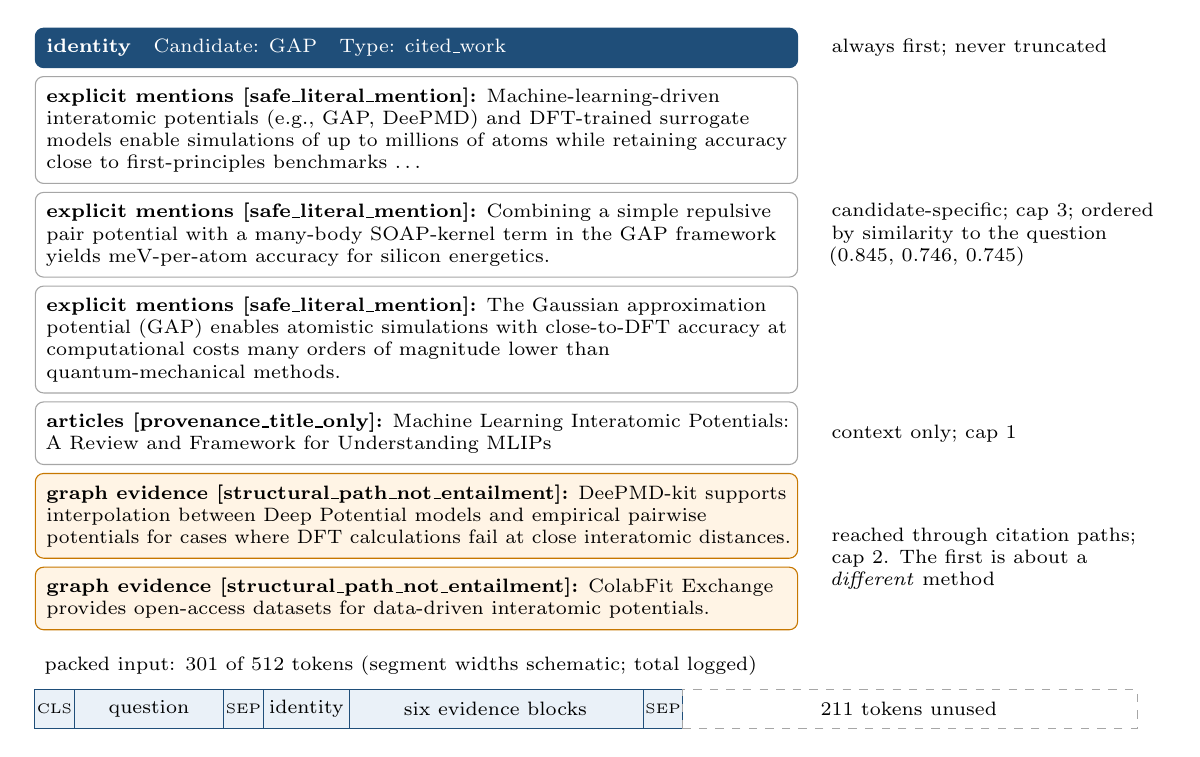
\begin{tikzpicture}[font=\scriptsize]
  \node[vdark,text width=9.4cm,align=flush left] (id) at (0,0) {\textbf{identity}\quad Candidate: GAP\quad Type: cited\_work};
  \node[vplain,text width=9.4cm,align=flush left,below=1mm of id] (b1) {\textbf{explicit mentions
     [safe\_literal\_mention]:} Machine-learning-driven interatomic potentials (e.g., GAP,
     DeePMD) and DFT-trained surrogate models enable simulations of up to millions of atoms
     while retaining accuracy close to first-principles benchmarks \dots};
  \node[vplain,text width=9.4cm,align=flush left,below=1mm of b1] (b2) {\textbf{explicit mentions
     [safe\_literal\_mention]:} Combining a simple repulsive pair potential with a many-body
     SOAP-kernel term in the GAP framework yields meV-per-atom accuracy for silicon
     energetics.};
  \node[vplain,text width=9.4cm,align=flush left,below=1mm of b2] (b3) {\textbf{explicit mentions
     [safe\_literal\_mention]:} The Gaussian approximation potential (GAP) enables atomistic
     simulations with close-to-DFT accuracy at computational costs many orders of magnitude
     lower than quantum-mechanical methods.};
  \node[vplain,text width=9.4cm,align=flush left,below=1mm of b3] (b4) {\textbf{articles
     [provenance\_title\_only]:} Machine Learning Interatomic Potentials: A Review and
     Framework for Understanding MLIPs};
  \node[vwarn,text width=9.4cm,align=flush left,below=1mm of b4] (b5) {\textbf{graph evidence
     [structural\_path\_not\_entailment]:} DeePMD-kit supports interpolation between Deep
     Potential models and empirical pairwise potentials for cases where DFT calculations
     fail at close interatomic distances.};
  \node[vwarn,text width=9.4cm,align=flush left,below=1mm of b5] (b6) {\textbf{graph evidence
     [structural\_path\_not\_entailment]:} ColabFit Exchange provides open-access datasets
     for data-driven interatomic potentials.};
  \node[anchor=west,text width=4.2cm,align=flush left] at ($(id.east)+(0.3,0)$) {always first; never truncated};
  \node[anchor=west,text width=4.2cm,align=flush left] at ($(b2.east)+(0.3,0)$) {candidate-specific; cap 3; ordered by
     similarity to the question (0.845, 0.746, 0.745)};
  \node[anchor=west,text width=4.2cm,align=flush left] at ($(b4.east)+(0.3,0)$) {context only; cap 1};
  \node[anchor=west,text width=4.2cm,align=flush left] at ($(b5.south east)+(0.3,0)$) {reached through citation paths; cap 2.
     The first is about a \emph{different} method};
  \coordinate (bar) at ($(b6.south west)+(0,-1.25)$);
  \draw[draw=accent,fill=soft] (bar) rectangle ++(8.23,0.5);
  \draw[draw=gray!70,dashed] ($(bar)+(8.23,0)$) rectangle ++(5.77,0.5);
  \foreach \dx in {0.5,2.4,2.9,4.0}{\draw[accent] ($(bar)+(\dx,0)$) -- ++(0,0.5);}
  \draw[accent] ($(bar)+(7.73,0)$) -- ++(0,0.5);
  \node at ($(bar)+(0.25,0.25)$) {\tiny CLS};
  \node at ($(bar)+(1.45,0.25)$) {question};
  \node at ($(bar)+(2.65,0.25)$) {\tiny SEP};
  \node at ($(bar)+(3.45,0.25)$) {identity};
  \node at ($(bar)+(5.85,0.25)$) {six evidence blocks};
  \node at ($(bar)+(7.98,0.25)$) {\tiny SEP};
  \node at ($(bar)+(11.1,0.25)$) {211 tokens unused};
  \node[anchor=west] at ($(bar)+(0,0.8)$) {packed input: 301 of 512 tokens (segment widths schematic; total logged)};
\end{tikzpicture}}
\caption[A query-dependent candidate card and its token packing]{A real candidate card: the entity GAP for question Q12, as stored in the frozen
cross-encoder trace (first block abridged). The card opens with the identity and continues
with evidence in priority order; orange blocks are structural context that the card itself
marks as not entailment. Thirty-eight further evidence rows were left out by family caps
and logged. The bar shows the model input: the question, a separator, and the card,
occupying 301 of the 512 available tokens. The cross-encoder returned a logit of $+1.296$
for this pair.}
\label{fig:card}
\end{figure}

\begin{algorithm}[!htbp]
\caption{Card construction and token packing for one candidate}
\label{alg:card}
\begin{algorithmic}[1]
\Require Entity $e$; similarities $\simop_q(\cdot)$; retained graph paths of $e$; caps; limit $L=512$
\Ensure Model input $(q',\ \text{document})$ and a log of included and omitted blocks
\State blocks $\gets[\ \text{identity}(e)\ ]$;\quad seen $\gets\emptyset$
\For{each family in priority order (\cref{tab:caps})}
  \State rows $\gets$ evidence linked to $e$ in this family (for graph evidence: path seeds)
  \State sort rows by $(-\simop_q,\ \text{candidate-specific first},\ \text{evidence id})$
  \For{each row with normalised text not in seen}
    \State add text to seen
    \If{fewer than cap blocks taken from this family} append block
    \Else\ log omission \code{family\_cap}
    \EndIf
  \EndFor
\EndFor
\State $q'\gets q_o$;\quad if $q_o$ leaves no room for the identity, truncate $q'$ (never the identity)
\State document $\gets$ identity text
\For{each evidence block in order}
  \If{tokens$(q',\ \text{document}+\text{block})\le L$} document $\gets$ document $+$ block
  \Else\ log this and all remaining blocks as \code{priority\_prefix\_token\_limit};\ \textbf{break}
  \EndIf
\EndFor
\State \Return $(q',\text{document})$, included blocks, omitted blocks, token count
\end{algorithmic}
\end{algorithm}

\paragraph{Measured card statistics.} Over the 1{,}800 question--candidate pairs that make
up the 100-candidate pools of all 18 questions, the packed input has between 54 and 512
tokens (median 176, mean 207.7). The median card has four blocks including the identity
and the largest has 19. In 81 pairs at least one block was dropped by the token limit; in
994 at least one row was left out by a family cap; the question was never truncated.
\Mtag{} (tabulated for this report from the frozen cross-encoder and evidence traces)

\begin{cautionbox}[A card can be almost empty]
Because most entities have only article titles attached (\cref{tab:index}), many cards
consist of an identity and one title. The cross-encoder then judges little more than a
name and a paper title, and its score reflects that poverty of evidence rather than the
entity's merit.
\end{cautionbox}

% ==================================================================
\section{The Complete A6 Algorithm}
\label{sec:algorithm}
% ==================================================================

\begin{algorithm}[!htbp]
\caption{A6 retrieval}
\label{alg:a6}
\begin{algorithmic}[1]
\Require Questions; graph $H$; frozen encoder $\phi$; frozen cross-encoder $f$; fixed configuration
\Ensure For each question a ranked list of canonical entities with full provenance; a freeze manifest
\State verify the SHA-256 of every pinned model file; fix seeds; set deterministic execution
\For{each distinct visibility cutoff $t$}
  \State $H_t\gets$ visible snapshot;\quad build entities, evidence links and arcs (\cref{sec:entities})
  \State encode node documents and evidence items with $\phi$ (cached by content hash)
\EndFor
\For{each question $q$}
  \State parse answer heads $A(q)$ and cutoff; build $q_o$ (verbatim) and $q_s$ (extractive)
  \State $\Ent_t(q)\gets$ entities whose types meet the answer families (all, if no head)
  \State compute $\simop_q(i)$ for every evidence item $i$ \Comment{\cref{eq:evsim}}
  \State $L_{\mathrm{do}},L_{\mathrm{ds}}\gets$ dense lists for $q_o$ and $q_s$ \Comment{\cref{eq:dense}}
  \State $L_{\mathrm{bm}}\gets$ BM25 on $q_o\oplus q_s$, positive scores only \Comment{\cref{eq:bm25}}
  \State $L_{\mathrm{nm}}\gets$ safe name and alias matches in $q_o$
  \State $L_{\mathrm{ev}}\gets$ owners of the 500 best evidence seeds \Comment{\cref{eq:evidence}}
  \State $L_{\mathrm{gr}}\gets$ bounded expansion from the 200 best seeds \Comment{\cref{alg:graph}}
  \State truncate each list to 500;\quad $F_q\gets$ union sorted by $(-\RRF,\ \text{entity id})$ \Comment{\cref{eq:rrf}}
  \State $P\gets$ first $K=100$ entities of $F_q$
  \For{each $e\in P$}
    \State build and pack $\mathrm{card}(e,q)$ within 512 tokens \Comment{\cref{alg:card}}
    \State $s_e\gets f(q_o,\ \mathrm{card}(e,q))$ \Comment{relevance logit}
  \EndFor
  \State $\pi_q\gets$ $P$ sorted by $(-s_e,\ \text{entity id})$, followed by $F_q[101{:}]$ unchanged \Comment{\cref{eq:final}}
  \State write $\pi_q$, per-channel ranks and scores, selected and omitted evidence, token counts
\EndFor
\State write predictions; compute their SHA-256; write the freeze manifest
\end{algorithmic}
\end{algorithm}

\paragraph{A note on how the frozen run computed this.} The frozen run scored a deeper
fused prefix once (configuration field \code{rerank\_k}${}=500$) and stored several
rankings derived from the same scores. The ranking defined by \cref{alg:a6} with $K=100$
is stored under the key \code{A6\_100}; depth 100 was a predeclared alternative to the
run's primary depth and was adopted for this supplement after the development results
were available (\cref{sec:k-status}). A card and its logit depend only on the question
and the candidate, not on the pool depth, so sorting the first 100 fused candidates by
those stored logits is the same computation as \cref{alg:a6}; the frozen file confirms
that this ranking's first 100 entries are a permutation of the fused top 100 and that
every later entry is in fused order. \Mtag

% ==================================================================
\section{Worked End-to-End Example}
\label{sec:worked}
% ==================================================================

This section follows one benchmark question through the whole system. Every candidate
name, rank and score below is read from the frozen \emph{prediction} traces, which were
written before any ground truth was loaded. Information about expected answers appears
only in the clearly marked evaluation illustration at the end.

\paragraph{Question (Q12).} ``What are the leading (by Feb 2026) ML-based interatomic
potential methods for large-scale atomistic simulation?''

\paragraph{Step 1: answer family and views.} The parser finds the head ``methods'', so
the admitted types are method, technique, component and cited\_work: 2{,}577 eligible
entities. The temporal phrase ``by Feb 2026'' resolves to the cutoff year 2026. The two
views are those of \cref{fig:views}.

\paragraph{Step 2: six lists.} Each list is computed independently of the others.
\Cref{tab:worked-channels} shows the top of each.

\begin{table}[!htbp]
\centering
\caption[Top entries of each first-stage list for Q12]{Top three entries of each first-stage list for Q12, with raw scores, from the
frozen channel trace. The lists disagree almost completely, and the raw scores are on
unrelated scales.}
\label{tab:worked-channels}
\small
\begin{tabularx}{\linewidth}{p{3.0cm}rX}
\toprule
List & Size & Top three (raw score)\\
\midrule
Dense, original & 500 & MatterSim (0.835); Oriented FAST and Rotated BRIEF (0.833); FIRE optimizer (0.830)\\
Dense, structured & 500 & MatterSim (0.807); Oriented FAST and Rotated BRIEF (0.801); FIRE optimizer (0.795)\\
BM25 & 500 & Large-scale atomistic simulation (18.61); Short-time MD simulation workflow (15.69); Type embedding (14.71)\\
Safe name & 1 & Large-scale atomistic simulation (32)\\
Evidence owner & 500 & Gaussian Approximation Potential (GAP) for silicon (0.856); Gaussian Approximation Potentials (0.852); Orb-v3 (0.852)\\
Bounded graph & 485 & the same three entities as the evidence list (0.856; 0.852; 0.852)\\
\bottomrule
\end{tabularx}
\end{table}

Three things are visible in the table. The dense lists place an unrelated
entity second, because its context document resembles the question. BM25 and the name
list are captured by an entity whose \emph{name} is the question's task phrase. The
evidence and graph lists are the ones that surface interatomic potentials.

\paragraph{Step 3: fusion.} The union has 1{,}438 entities. The fused top three are
Gaussian Approximation Potentials (0.0675), MatterSim (0.0628) and Large-scale atomistic
simulation (0.0580). The first of these is in no list's top spot but is ranked 13, 14,
64, 2 and 2 across five lists:
\[
  \tfrac{1}{73}+\tfrac{1}{74}+\tfrac{1}{124}+\tfrac{1}{62}+\tfrac{1}{62}=0.0675 .
\]

\paragraph{Step 4: one candidate in detail.} Consider the entity \textbf{GAP}, a single
\code{cited\_work} node. \Cref{fig:worked} traces it.

\begin{figure}[H]
\centering
\fitfig{%
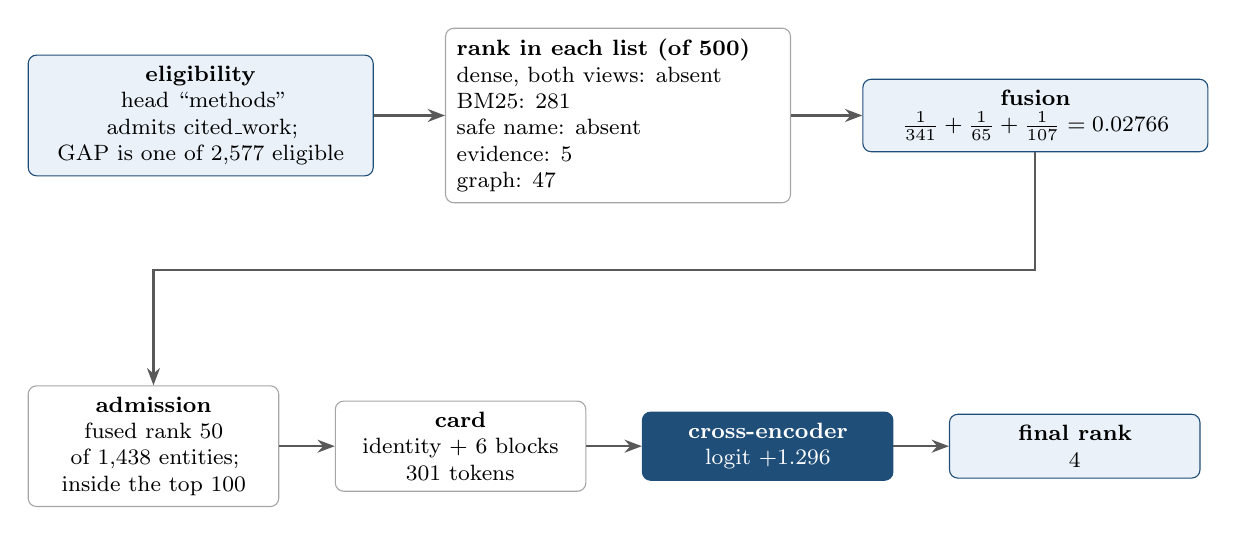
\begin{tikzpicture}[font=\footnotesize]
  \node[vbox,text width=4.1cm] (a1) at (0,0) {\textbf{eligibility}\\ head ``methods''\\ admits cited\_work;\\ GAP is one of 2{,}577 eligible};
  \node[vplain,text width=4.1cm,align=flush left] (a2) at (5.3,0) {\textbf{rank in each list (of 500)}\\ dense, both views: absent\\
     BM25: 281\\ safe name: absent\\ evidence: 5\\ graph: 47};
  \node[vbox,text width=4.1cm] (a3) at (10.6,0) {\textbf{fusion}\\ $\frac{1}{341}+\frac{1}{65}+\frac{1}{107}=0.02766$};
  \node[vplain,text width=2.9cm] (b1) at (-0.6,-4.2) {\textbf{admission}\\ fused rank 50\\ of 1{,}438 entities;\\ inside the top 100};
  \node[vplain,text width=2.9cm] (b2) at (3.3,-4.2) {\textbf{card}\\ identity + 6 blocks\\ 301 tokens};
  \node[vdark,text width=2.9cm] (b3) at (7.2,-4.2) {\textbf{cross-encoder}\\ logit $+1.296$};
  \node[vbox,text width=2.9cm] (b4) at (11.1,-4.2) {\textbf{final rank}\\ 4};
  \draw[varr] (a1)--(a2); \draw[varr] (a2)--(a3);
  \draw[varr] (a3.south) -- ++(0,-1.5) -| (b1.north);
  \draw[varr] (b1)--(b2); \draw[varr] (b2)--(b3); \draw[varr] (b3)--(b4);
\end{tikzpicture}}
\caption[One candidate traced through A6]{One candidate's path through A6 for question Q12, with every number taken from
the frozen prediction traces. The entity GAP is invisible to dense retrieval (a three-letter
name with little context) and weak in BM25. The evidence channel ranks it fifth because a
claim that literally mentions GAP matches the question, and the graph channel reaches it
through citing articles. Fusion admits it at rank 50; the cross-encoder, reading the card
of \cref{fig:card}, moves it to rank 4.}
\label{fig:worked}
\end{figure}

\paragraph{Step 5: the reranked head.}

\begin{table}[!htbp]
\centering
\caption[Final top ten for Q12]{Final top ten for Q12 from the frozen predictions, with the fused rank each
entity had before reranking, its relevance logit and its packed length. Logits order
candidates within this question only. For comparison, the two lowest logits in the pool
are $-7.76$ and $-10.08$.}
\label{tab:worked-final}
\small
\begin{tabularx}{\linewidth}{rXlrrr}
\toprule
Final & Entity & Types & Fused & Logit & Tokens\\
\midrule
1 & Large-scale atomistic simulation & technique & 3 & $+2.840$ & 63\\
2 & Deep Molecular Dynamics & method & 32 & $+1.766$ & 214\\
3 & ML-IAP & method & 49 & $+1.523$ & 205\\
4 & GAP & cited\_work & 50 & $+1.296$ & 301\\
5 & DFT & cited\_work & 80 & $+1.265$ & 238\\
6 & unconstrained MLIP evaluation framework & method & 52 & $+1.263$ & 483\\
7 & Gaussian Approximation Potentials & cited\_work, method & 1 & $+1.010$ & 237\\
8 & DeepMD & cited\_work & 62 & $+0.794$ & 313\\
9 & Machine Learning Interatomic Potentials & method & 11 & $+0.692$ & 117\\
10 & MatterSim & cited\_work, method & 2 & $+0.622$ & 256\\
\bottomrule
\end{tabularx}
\end{table}

The table shows the reranker working and failing in the same list.
\begin{itemize}
  \item \textbf{It removes a spurious candidate.} ``Oriented FAST and Rotated BRIEF'', second
        in both dense lists and seventh after fusion, receives a logit of $-4.04$ and falls
        to rank 77. Its card holds an identity and one article title.
  \item \textbf{It promotes evidenced candidates.} GAP rises from 50 to 4 and DeepMD from 62
        to 8, both on the strength of claims that mention them.
  \item \textbf{It rewards echo.} The top result is a \emph{technique} entity whose name
        repeats the question's task phrase. Its card has 63 tokens. A relevance model
        trained on web search rates a passage that restates the query as highly relevant;
        it has no notion that the question asks for a potential and not for a task.
  \item \textbf{It ranks near-duplicates separately.} ``GAP'' and ``Gaussian Approximation
        Potentials'', and ``DeepMD'' and ``Deep Molecular Dynamics'', are distinct canonical
        entities (\cref{fig:entity}) and occupy four of the top eight places.
\end{itemize}

\begin{cautionbox}[Evaluation illustration (computed after the freeze)]
The evaluator, run afterwards in a separate process, maps 13 expected methods for Q12 to
graph identities. All 13 are in the 100-candidate pool. Three are in the final top ten:
GAP (4), DeePMD (8, the entity named DeepMD) and MatterSim (10); their fused ranks were
50, 62 and 2. The entities at ranks 2 and 7 appear to denote the same methods as two of
those targets but have different surface forms, so they receive no credit. No expert
adjudicated whether any non-credited candidate is a wrong answer.
\end{cautionbox}

% ==================================================================
\section{Temporal and Hypergraph Integrity}
\label{sec:temporal}
% ==================================================================

V2 retrieves from a temporal hypergraph, so it must respect time and it must be clear
about what it does with hyperedges.

\subsection{Visibility}

V2 uses the main report's strict visibility rule without modification.

\begin{definition}[Visibility, inherited]
A node $v$ is visible at year $t$ iff $\mathrm{first\_seen\_year}(v)\le t$. A hyperedge
is visible at $t$ iff its \code{year} is at most $t$, the publication year of the article
asserting it (when recorded) is at most $t$, and every one of its members is visible.
\end{definition}

\code{first\_seen\_year} is the publication year of the earliest corpus paper mentioning
the node; it is used instead of \code{origin\_year} so that the snapshot contains only
what the \emph{corpus} had seen. Everything downstream inherits the filter: entities are
built from visible nodes, evidence links and arcs from visible hyperedges, and an entity's
year is the earliest of its members'. Graph aliases carry no dates, so an alias is used
only if its node was last seen no later than the cutoff. \Gtag{} (tested by
\path{test_temporal_visibility_applies_to_nodes_edges_aliases})

The cutoff comes from the question. A phrase such as ``by Feb 2026'' is recognised by a
date pattern and reduced to its year; ``before $Y$'' becomes $Y-1$; the cutoff is the
smaller of that year and the configured snapshot (2026). All 18 benchmark questions
resolve to 2026, so the frozen run uses a single index. \Mtag

\begin{cautionbox}[Year-level temporal precision]
The data carry years, not dates. ``By February 2026'' is therefore enforced as ``by the
end of 2026'': the system \emph{cannot} exclude material that appeared between March and
December 2026. The pretrained models are not historically versioned either, so their
parameters may encode knowledge from any time before their own training. This limitation
is inherited from the main report and is not solved here.
\end{cautionbox}

\subsection{Provenance}

Every evidence link and every graph path stores the hyperedge id, the relation type, the
edge year and the edge's provenance record (source and asserting article). Every evidence
block placed on a card stores its node id, its first-seen year and its provenance. A
ranked answer can therefore be traced back to the hyperedges and papers that produced the
text the model read.

\subsection{What V2 does and does not do with hyperedges}

It is important not to blur two different uses of the hypergraph.

\begin{itemize}
  \item \textbf{The hierarchy's native hyperedge coarsening (P4, T4)} is a rule for what a
        hyperedge becomes when its endpoints are merged into super-nodes, and the
        hierarchy's objective uses that rule. It lives in the main system. \textbf{V2 does
        not redefine, re-implement or evaluate it.}
  \item \textbf{V2's evidence links and graph expansion} read native hyperedges as they
        are. A hyperedge of arity $n$ is interpreted through its role pattern (one method
        and its typed targets; one article, one claim and at most one method), not through
        a pairwise projection and not through arbitrary co-membership. This supplies
        structured, provenance-bearing evidence to retrieval. It is a reading of the
        graph, not a coarsening of it.
\end{itemize}

The cross-encoder itself is not hypergraph-native in any sense. It is a text model. The
graph's contribution is upstream of it: deciding which entities exist, which evidence
belongs to which entity, and which entities are structurally near question-relevant text.

% ==================================================================
\section{Leakage Prevention}
\label{sec:leakage}
% ==================================================================

Evaluation validity carries the largest weight in the assessment. For a retrieval
benchmark the central threat is leakage: any route by which the expected answers could
influence the predictions. V2 treats the question text as legitimate input and the
answers as evaluation-only, and enforces the distinction mechanically.

\begin{figure}[!htbp]
\centering
\fitfig{%
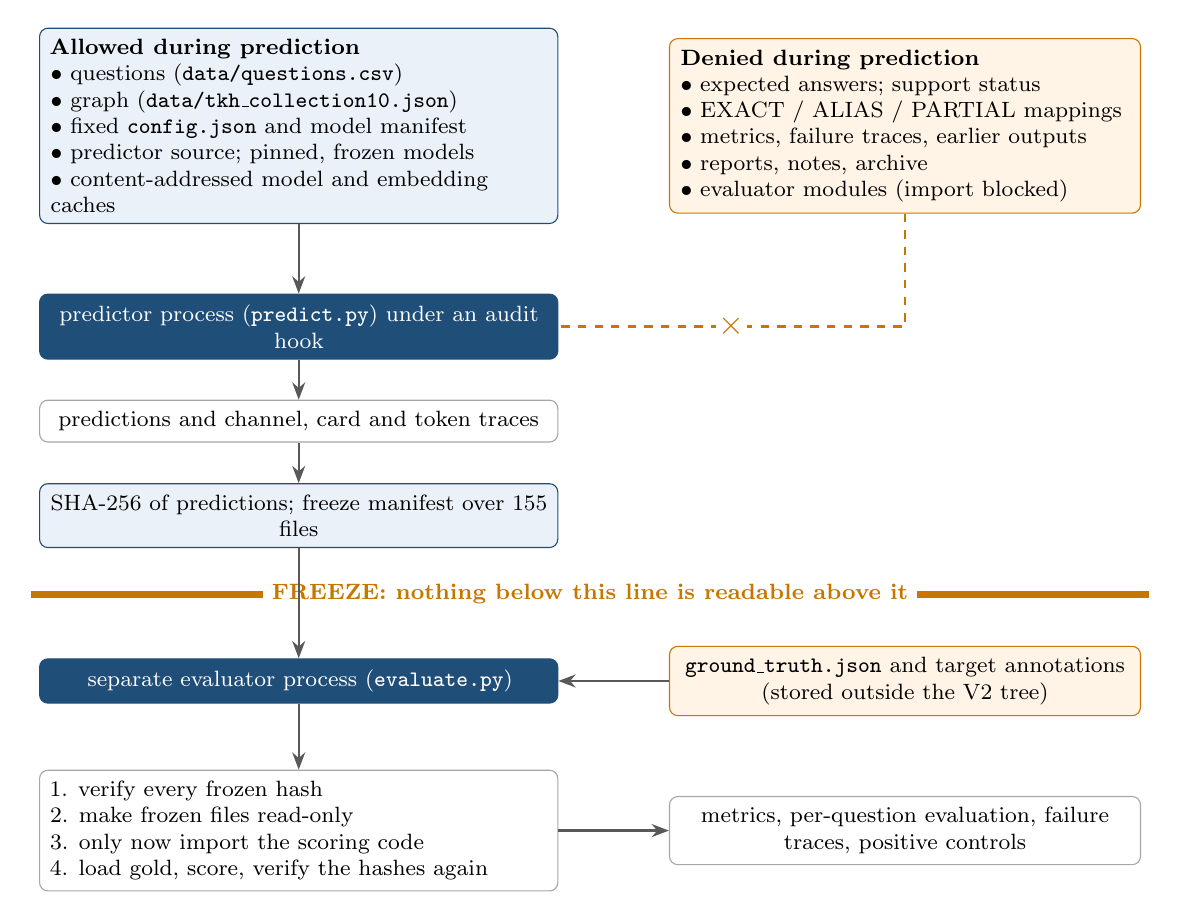
\begin{tikzpicture}[font=\footnotesize]
  \node[vbox,text width=6.3cm,align=flush left] (in) at (0,0) {\textbf{Allowed during prediction}\\
     $\bullet$ questions (\texttt{data/questions.csv})\\
     $\bullet$ graph (\texttt{data/tkh\_collection10.json})\\
     $\bullet$ fixed \texttt{config.json} and model manifest\\
     $\bullet$ predictor source; pinned, frozen models\\
     $\bullet$ content-addressed model and embedding caches};
  \node[vwarn,text width=5.7cm,align=flush left] (den) at (7.7,0) {\textbf{Denied during prediction}\\
     $\bullet$ expected answers; support status\\
     $\bullet$ EXACT / ALIAS / PARTIAL mappings\\
     $\bullet$ metrics, failure traces, earlier outputs\\
     $\bullet$ reports, notes, archive\\
     $\bullet$ evaluator modules (import blocked)};
  \node[vdark,text width=6.3cm] (pred) at (0,-2.55) {predictor process (\texttt{predict.py}) under an audit hook};
  \node[vplain,text width=6.3cm] (out) at (0,-3.75) {predictions and channel, card and token traces};
  \node[vbox,text width=6.3cm] (sha) at (0,-4.95) {SHA-256 of predictions; freeze manifest over 155 files};
  \draw[varr] (in)--(pred); \draw[varr] (pred)--(out); \draw[varr] (out)--(sha);
  \draw[warnline,dashed,line width=1pt] (den.south) |- node[pos=0.75,fill=white,inner sep=1pt,text=warnline] {\large$\times$} (pred.east);
  \draw[warnline,line width=2.4pt] (-3.4,-5.95) -- (10.8,-5.95);
  \node[fill=white,text=warnline,font=\footnotesize\bfseries] at (3.7,-5.95) {FREEZE: nothing below this line is readable above it};
  \node[vdark,text width=6.3cm] (ev) at (0,-7.05) {separate evaluator process (\texttt{evaluate.py})};
  \node[vplain,text width=6.3cm,align=flush left] (steps) at (0,-8.95) {1. verify every frozen hash\\ 2. make frozen files read-only\\
     3. only now import the scoring code\\ 4. load gold, score, verify the hashes again};
  \node[vwarn,text width=5.7cm] (gold) at (7.7,-7.05) {\texttt{ground\_truth.json} and target annotations\\ (stored outside the V2 tree)};
  \node[vplain,text width=5.7cm] (met) at (7.7,-8.95) {metrics, per-question evaluation, failure traces, positive controls};
  \draw[varr] (sha)--(ev); \draw[varr] (gold)--(ev); \draw[varr] (ev)--(steps); \draw[varr] (steps)--(met);
\end{tikzpicture}}
\caption[Prediction/evaluation firewall and SHA-256 freeze]{The prediction/evaluation firewall. Above the orange line a single process may
read only the inputs listed on the left; any attempt to open a file in the right-hand
list, or to import an evaluator module, raises an error. The process ends by hashing its
output. Below the line a different process first checks those hashes, protects the frozen
files against modification, and only then imports the code that reads the ground truth.
Information flows downward only.}
\label{fig:firewall}
\end{figure}

\subsection{What the prediction phase may and may not see}

The predictor may read the question text, the TKH, the pretrained model weights and the
fixed configuration. It may \emph{not} read expected answers, target support status, the
EXACT/ALIAS/PARTIAL mappings, final metrics, failure traces, or any earlier evaluated
output.

This is enforced by a Python audit hook installed before any project code is imported.
\Gtag{} (for file access through Python)
\begin{itemize}
  \item \textbf{Read allowlist.} Inside the V2 tree a read is permitted only for
        \path{config.json}, \path{model_manifest.json}, the two files in \path{data/}, the
        predictor's own source, files the process itself created, and the model and
        embedding caches. Everything else is refused.
  \item \textbf{Forbidden categories.} Any path containing \code{ground\_truth},
        \code{target\_annotations}, \code{metrics}, \code{failure}, \code{oracle},
        \code{positive\_controls} and similar markers, and the directories \path{report/},
        \path{notes/}, \path{archive/} and \path{artifacts/evaluation/}, are refused even
        if a path were otherwise allowed.
  \item \textbf{Outside the tree.} The ground truth lives in the main package, not in V2.
        Any read of a repository file outside V2, other than installed third-party
        packages, is refused.
  \item \textbf{Import guard.} Importing a module whose name marks it as evaluation code
        raises an error before the freeze.
  \item \textbf{Fail closed.} The run asserts at the end that no access was denied; one
        denied access aborts the freeze.
\end{itemize}

\paragraph{Measured audit.} The frozen run logged 4{,}186 project file reads, 0 denied
reads, 0 gold reads and 0 reads of earlier evaluation results, and imported 15 local
modules, none of them evaluation code. \Mtag

\subsection{Frozen models and no fitting}

\begin{itemize}
  \item \textbf{No fine-tuning.} Both models are used with their published weights; their
        files are hash-checked against the manifest before every run. \Gtag
  \item \textbf{No training on benchmark answers.} No component has parameters learned
        from this benchmark.
  \item \textbf{No learned fusion weights.} Fusion is the unweighted sum of
        \cref{eq:rrf}.
  \item \textbf{No thresholds fitted to ground-truth rankings.} The constants $k=60$,
        $k_1=1.5$, $b=0.75$, the list depth, the seed depths, the graph caps and the card
        caps are fixed in \path{config.json}, and the configuration file is part of the
        hashed freeze. \Dtag{} The one exception is the reranking depth: $K=100$ was
        chosen among predeclared depths after development results were available
        (\cref{sec:k-status}).
\end{itemize}

\subsection{Freeze, then score}

When the last question is processed, the predictor writes the predictions, computes their
SHA-256 and writes a manifest containing the hash of 155 files: the configuration, the
model manifest, the input data, the predictor source and every prediction and trace file.
It records a \code{predictions\_frozen} event and exits.

The evaluator is a different program run as a different process. Its import order is the
safeguard: it imports only hashing utilities, verifies the predictions hash and all 155
file hashes, installs a guard that refuses any write, delete, rename or permission change
on a frozen file, and only then imports the scoring module that knows where the ground
truth is. After scoring it verifies the hashes once more. \Gtag{} (tested by
\path{test_evaluation_freeze_refuses_tampering} and
\path{test_new_prediction_integrity_and_phase_order})

\begin{keybox}[Freeze first, score second]
Predictions are finalised and hashed before evaluation code can read gold.
\end{keybox}

\begin{figure}[!htbp]
\centering
\fitfig{%
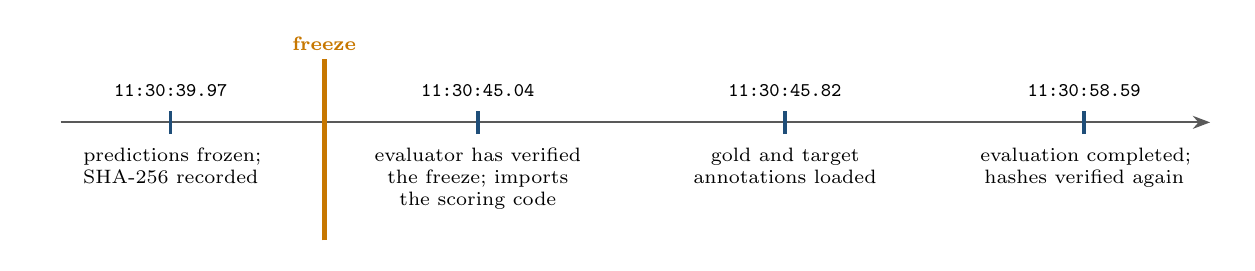
\begin{tikzpicture}[font=\scriptsize]
  \draw[vline,-{Stealth[length=2.2mm]}] (0,0) -- (14.6,0);
  \foreach \x/\ts/\txt in {1.4/{11:30:39.97}/{predictions frozen;\\ SHA-256 recorded},
       5.3/{11:30:45.04}/{evaluator has verified\\ the freeze; imports\\ the scoring code},
       9.2/{11:30:45.82}/{gold and target\\ annotations loaded},
       13.0/{11:30:58.59}/{evaluation completed;\\ hashes verified again}}{
    \draw[accent,line width=1.2pt] (\x,-0.15) -- (\x,0.15);
    \node[above,font=\scriptsize\ttfamily] at (\x,0.2) {\ts};
    \node[below,align=flush center,text width=3.4cm] at (\x,-0.2) {\txt};
  }
  \draw[warnline,line width=1.6pt] (3.35,-1.5) -- (3.35,0.8);
  \node[text=warnline,font=\scriptsize\bfseries] at (3.35,1.0) {freeze};
\end{tikzpicture}}
\caption[Recorded order of freeze and evaluation events]{The order of events recorded in the run's own event log (UTC, 2 October 2026;
spacing not to scale). The ground truth is first opened 5.85 seconds \emph{after} the
predictions were hashed, and the hash recorded when evaluation completes equals the hash
recorded at the freeze. The same log shows that only one gold-loading event occurred.}
\label{fig:timeline}
\end{figure}

\paragraph{Measured integrity.} The predictions hash is
\begin{center}
\code{2d7485f1d0ecfb541d1d83413e2ac1d9}\\
\code{61519ce9c1e0870dbd74311462918570}
\end{center}
at the freeze, at evaluation start, at evaluation end, and for a second full execution of
the predictor into a separate directory. \Mtag{} That second execution reused cached model
outputs, so it demonstrates deterministic assembly, not an independent repetition of
neural inference.

\subsection{What the firewall does not establish}

\begin{cautionbox}[Limits of the isolation]
\begin{itemize}[leftmargin=*]
  \item \textbf{Design-time exposure.} The benchmark was evaluated in earlier development
        iterations, and those results informed human design decisions. The firewall blocks
        access \emph{while a prediction runs}; it cannot make the benchmark unseen.
  \item \textbf{Configuration chosen with results visible.} Among the predeclared
        reranking depths evaluated during development (100, 200 and 500), $K=100$ gave
        the strongest observed top-10 recovery. This supplement describes that simplified
        configuration. This selection was made after development results were available
        and is therefore a development choice, not an independently validated optimum.
  \item \textbf{Cooperative, not hostile-proof.} A Python audit hook observes file access
        made through Python. It is not an operating-system sandbox and would not contain
        deliberately adversarial native code.
  \item \textbf{Interrupted attempts.} The event log records three prediction starts; only
        the last completed and froze. No evaluation ran between them.
\end{itemize}
\end{cautionbox}

% ==================================================================
\section{Evaluation Protocol}
\label{sec:protocol}
% ==================================================================

\subsection{Targets and their status}

The benchmark has 18 questions. The 14 Type-A questions list expected methods, giving 63
target occurrences. Identity metrics are computed on these 14; predictions are produced
for all 18. Before a target can be scored it must be mapped to the graph, and that mapping
is itself uncertain. Each occurrence has one status, assigned by the evaluator after the
freeze using the main package's audited annotations.

\begin{table}[!htbp]
\centering
\caption[Target-status categories]{Target-status categories. These are evaluation concepts: no status, and no
mapping, is available to the predictor. \Mtag{} Counts from the frozen \code{metrics.json}.}
\label{tab:status}
\small
\begin{tabularx}{\linewidth}{lrXl}
\toprule
Status & Count & Meaning & Direct credit\\
\midrule
EXACT & 48 & A node's surface form equals the target after normalisation, whatever its type & yes\\
ALIAS & 1 & The same identity appears in the graph under a different name (annotated) & yes\\
PARTIAL & 11 & Only a related or narrower node exists, e.g.\ ``E(3)-equivariant GNNs'' & no\\
COMPOSITE & 1 & The target is a combination whose parts are separate nodes & no\\
ABSENT & 2 & No defensible mapping was found, e.g.\ ``MACE-F'' & no\\
\midrule
Total & 63 & of which directly mapped (EXACT + ALIAS): \textbf{49} & \\
\bottomrule
\end{tabularx}
\end{table}

Three rules follow, and each lowers the attainable score. \Gtag
\begin{itemize}
  \item \textbf{PARTIAL is not promoted to success.} Retrieving a related node is not
        retrieving the expected identity.
  \item \textbf{ABSENT cannot receive identity credit.} There is nothing in the graph to
        retrieve.
  \item \textbf{COMPOSITE is reported separately.} A composite target counts only if every
        component is retrieved, and it is never mixed into the direct counts.
\end{itemize}

\begin{cautionbox}[Gold incompleteness and the recall ceiling]
Because 14 of the 63 occurrences are not directly mapped, final recall can never exceed
$49/63=0.778$, even for a perfect retriever. Two questions (Q5 and Q11) have no directly
mapped target at all and contribute zero by construction. The mapping was produced by
automatic matching and assistant inspection; no domain expert adjudicated it. ABSENT
means ``no mapping found'', not ``proven absent''.
\end{cautionbox}

\subsection{Metrics}

\begin{description}[leftmargin=0.5cm,style=nextline]
  \item[Candidate recall@$K$ (\cref{def:candrecall})] Mapped targets with at least one
        mapped entity in the fused top $K$, before reranking, divided by 49.
  \item[Final recall R@$k$ (\cref{def:recall})] Mapped targets ranked within $k$, divided
        by all 63 occurrences, for $k\in\{1,5,10,25,50,100\}$. A target mapped to several
        entities takes its best rank.
  \item[Mapped-only recall] The same numerator divided by 49; reported as a secondary
        view that removes the mapping ceiling.
  \item[Mean reciprocal rank]
        \begin{equation}
          \mathrm{MRR}=\frac{1}{14}\sum_{q\in\text{Type A}}\frac{1}{\min_{\tau\in\mathcal T_{\mathrm{dir}}(q)}\rank_{\pi_q}(\tau)},
        \end{equation}
        with a term of zero when a question has no mapped target or none is ranked. The
        denominator is always 14.
  \item[Observed and missing ranks] The median and mean rank of mapped targets that
        receive a rank, and the number that receive none because they never enter the
        union.
\end{description}

\subsection{Is the evaluator itself sound?}

A low score could come from a scoring bug. The evaluator therefore runs a positive
control, kept separate from all retrieval results: for each question it builds a ranking
containing exactly the mapped identities and checks that every one is counted. All 49 are
recovered. \Mtag{} The control is labelled as gold-informed and evaluation-only and is
never reported as a retrieval result.

% ==================================================================
\section{Results}
\label{sec:results}
% ==================================================================

\begin{cautionbox}[Development diagnostics, not held-out performance]
Every number in this section comes from the development benchmark, which was inspected
during the design of both V1 and V2. The run is a single deterministic execution on 14
scored questions. The numbers describe this system on this benchmark; they are not
estimates of performance on unseen questions, and they carry no confidence intervals.
\end{cautionbox}

\subsection{Headline numbers}

\begin{table}[!htbp]
\centering
\caption[A6 results (development diagnostics)]{\textbf{Development diagnostics.} A6 with a reranking pool of $K=100$, frozen
ranking key \code{A6\_100}. Recall counts directly mapped targets ranked within $k$; the
main column divides by all 63 target occurrences, the secondary column by the 49 that are
mapped. Source: frozen \code{artifacts/evaluation/metrics.json}.}
\label{tab:results}
\begin{tabular}{lrrr}
\toprule
Metric & Hits & Recall (of 63) & Mapped-only (of 49)\\
\midrule
R@1 & 1 & 0.0159 & 0.0204\\
R@5 & 6 & 0.0952 & 0.1224\\
R@10 & 12 & 0.1905 & 0.2449\\
R@25 & 18 & 0.2857 & 0.3673\\
R@50 & 25 & 0.3968 & 0.5102\\
R@100 & 37 & 0.5873 & 0.7551\\
\midrule
MRR (14 questions) & & 0.1669 & \\
\midrule
Candidate recall@100 (pool) & 37 & & 0.7551\\
Candidate recall, full union & 46 & & 0.9388\\
Mapped targets with a final rank & 46 & \multicolumn{2}{l}{median rank 40, mean 77.7}\\
Mapped targets never ranked & 3 & \multicolumn{2}{l}{all removed by the answer-family filter}\\
\bottomrule
\end{tabular}
\end{table}

\begin{figure}[!htbp]
\centering
\fitfig{%
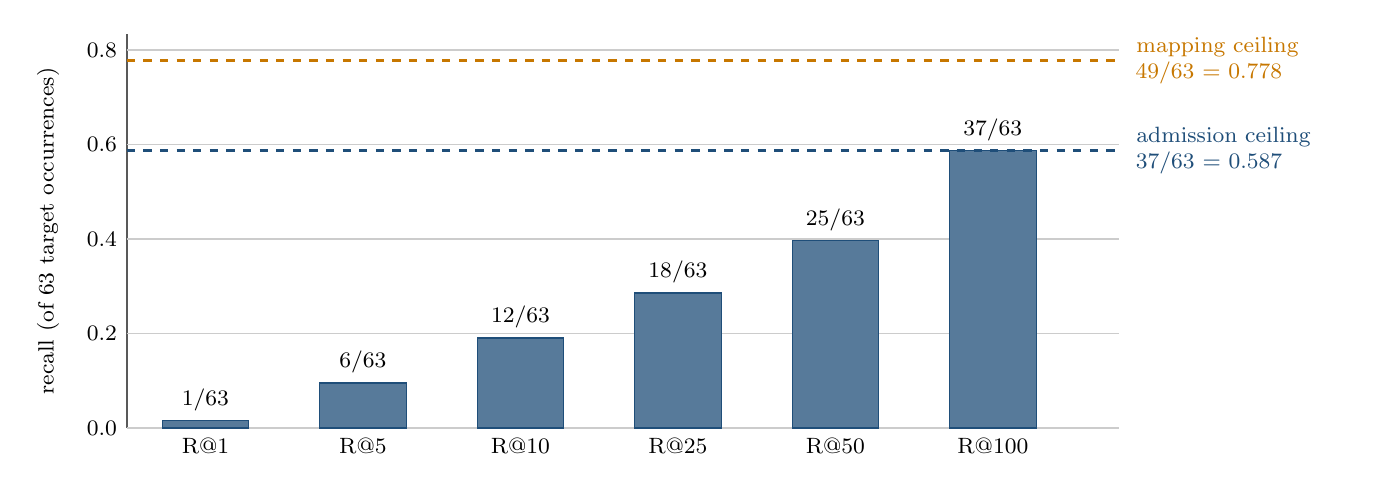
\begin{tikzpicture}[font=\footnotesize]
  % axes
  \draw[vline] (0,0) -- (12.6,0);
  \draw[vline] (0,0) -- (0,5.0);
  \foreach \y/\lab in {0/0.0,1.2/0.2,2.4/0.4,3.6/0.6,4.8/0.8}{
    \draw[gray!40] (0,\y) -- (12.6,\y);
    \node[left] at (0,\y) {\lab};
  }
  \node[rotate=90] at (-1.0,2.5) {recall (of 63 target occurrences)};
  % bars: height = recall * 6
  \foreach \x/\barh/\kk/\cnt in {1.0/0.095/1/{1},3.0/0.571/5/{6},5.0/1.143/10/{12},7.0/1.714/25/{18},9.0/2.381/50/{25},11.0/3.524/100/{37}}{
    \draw[draw=accent,fill=accent!75] (\x-0.55,0) rectangle (\x+0.55,\barh);
    \node[above] at (\x,\barh) {\cnt/63};
    \node[below] at (\x,0) {R@\kk};
  }
  \draw[warnline,dashed,line width=1pt] (0,4.667) -- (12.6,4.667);
  \node[anchor=west,text=warnline,text width=2.7cm,align=flush left] at (12.7,4.667) {mapping ceiling\\ 49/63 = 0.778};
  \draw[accent,dashed,line width=1pt] (0,3.524) -- (12.6,3.524);
  \node[anchor=west,text=accent,text width=2.7cm,align=flush left] at (12.7,3.524) {admission ceiling\\ 37/63 = 0.587};
\end{tikzpicture}}
\caption[Final recall at six cut-offs (development diagnostics)]{\textbf{Development diagnostics.} Final recall of A6 ($K=100$) at six cut-offs,
as a fraction of all 63 target occurrences, with the hit count above each bar. Two
ceilings bound the bars. No ranking could exceed the orange line, because 14 targets have
no direct graph identity. This system cannot exceed the blue line at any $k\le100$,
because only 37 mapped targets are admitted to the pool; R@100 meets that line exactly, as
\cref{prop:ceiling} requires.}
\label{fig:recall-bars}
\end{figure}

\subsection{Where targets are lost}

\Cref{fig:result-funnel} follows the 63 target occurrences through the system. Each step
removes targets for a different reason, and the reasons call for different remedies:
unmapped targets are a property of the benchmark and the graph, the type filter is a
design choice, fusion depth belongs to the admission stage, and the last step is the
ordering stage.

\begin{figure}[H]
\centering
\fitfig{%
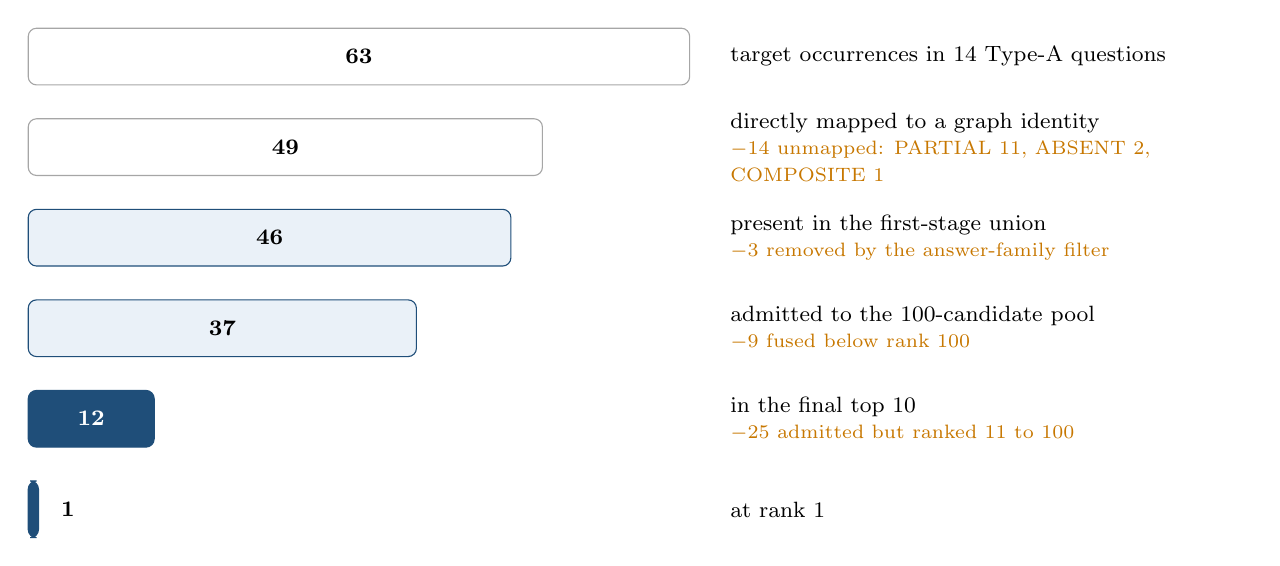
\begin{tikzpicture}[font=\footnotesize]
  % bar length = count * (8.4/63) cm
  \node[vplain,minimum width=8.40cm,minimum height=0.72cm,anchor=west,inner sep=0pt] at (0,0) {\textbf{63}};
  \node[vplain,minimum width=6.53cm,minimum height=0.72cm,anchor=west,inner sep=0pt] at (0,-1.15) {\textbf{49}};
  \node[vbox,minimum width=6.13cm,minimum height=0.72cm,anchor=west,inner sep=0pt] at (0,-2.3) {\textbf{46}};
  \node[vbox,minimum width=4.93cm,minimum height=0.72cm,anchor=west,inner sep=0pt] at (0,-3.45) {\textbf{37}};
  \node[vdark,minimum width=1.60cm,minimum height=0.72cm,anchor=west,inner sep=0pt] at (0,-4.6) {\textbf{12}};
  \node[vdark,minimum width=0.13cm,minimum height=0.72cm,anchor=west,inner sep=0pt] at (0,-5.75) {};
  \node[anchor=west] at (0.3,-5.75) {\textbf{1}};
  \node[anchor=west,text width=6.5cm,align=flush left] at (8.8,0) {target occurrences in 14 Type-A questions};
  \node[anchor=west,text width=6.5cm,align=flush left] at (8.8,-1.15) {directly mapped to a graph identity\\
     {\scriptsize\color{warnline}$-14$ unmapped: PARTIAL 11, ABSENT 2, COMPOSITE 1}};
  \node[anchor=west,text width=6.5cm,align=flush left] at (8.8,-2.3) {present in the first-stage union\\
     {\scriptsize\color{warnline}$-3$ removed by the answer-family filter}};
  \node[anchor=west,text width=6.5cm,align=flush left] at (8.8,-3.45) {admitted to the 100-candidate pool\\
     {\scriptsize\color{warnline}$-9$ fused below rank 100}};
  \node[anchor=west,text width=6.5cm,align=flush left] at (8.8,-4.6) {in the final top 10\\
     {\scriptsize\color{warnline}$-25$ admitted but ranked 11 to 100}};
  \node[anchor=west,text width=6.5cm,align=flush left] at (8.8,-5.75) {at rank 1};
\end{tikzpicture}}
\caption[Target loss by stage (development diagnostics)]{\textbf{Development diagnostics.} The loss of targets stage by stage; bar length
is proportional to the count. Fourteen targets are unreachable for any system because the
graph holds no direct identity for them. Three are removed by the hard answer-family
filter. Nine are in the union but fused below rank 100. Of the 37 admitted, 25 are not
brought into the top ten by the cross-encoder. The largest single loss is in ordering, not
in admission.}
\label{fig:result-funnel}
\end{figure}

\subsection{What the reranking stage changed}

Because A6 is its own first stage plus one reranking step, comparing the order before and
after that step isolates what the cross-encoder contributes. Both rows of
\cref{tab:rerank-effect} are states of the same pipeline on the same pool.

\begin{table}[H]
\centering
\caption[Effect of the reranking step (development diagnostics)]{\textbf{Development diagnostics.} Mapped-target hits before and after the
reranking step of A6, out of 63. R@100 is identical by \cref{prop:ceiling}.}
\label{tab:rerank-effect}
\small
\begin{tabular}{lrrrrrrr}
\toprule
Order & @1 & @5 & @10 & @25 & @50 & @100 & MRR\\
\midrule
Fused order (input to the cross-encoder) & 0 & 4 & 6 & 11 & 29 & 37 & 0.1554\\
Final order (after the cross-encoder) & 1 & 6 & 12 & 18 & 25 & 37 & 0.1669\\
\bottomrule
\end{tabular}
\end{table}

Among the 37 admitted targets, 17 moved up and 20 moved down; none stayed in place. Seven
entered the top ten and one left it. The median rank of admitted targets improved from 36
to 27. \Mtag{} The reranker improves the head of the list (hits at 10 double, from 6 to
12) but it is not uniformly beneficial: hits at 50 fall from 29 to 25, because some
admitted targets are pushed toward the bottom of the pool. The largest such move is MACE
for Q12, from fused rank 42 to final rank 86. \Mtag

\begin{figure}[!htbp]
\centering
\fitfig{%
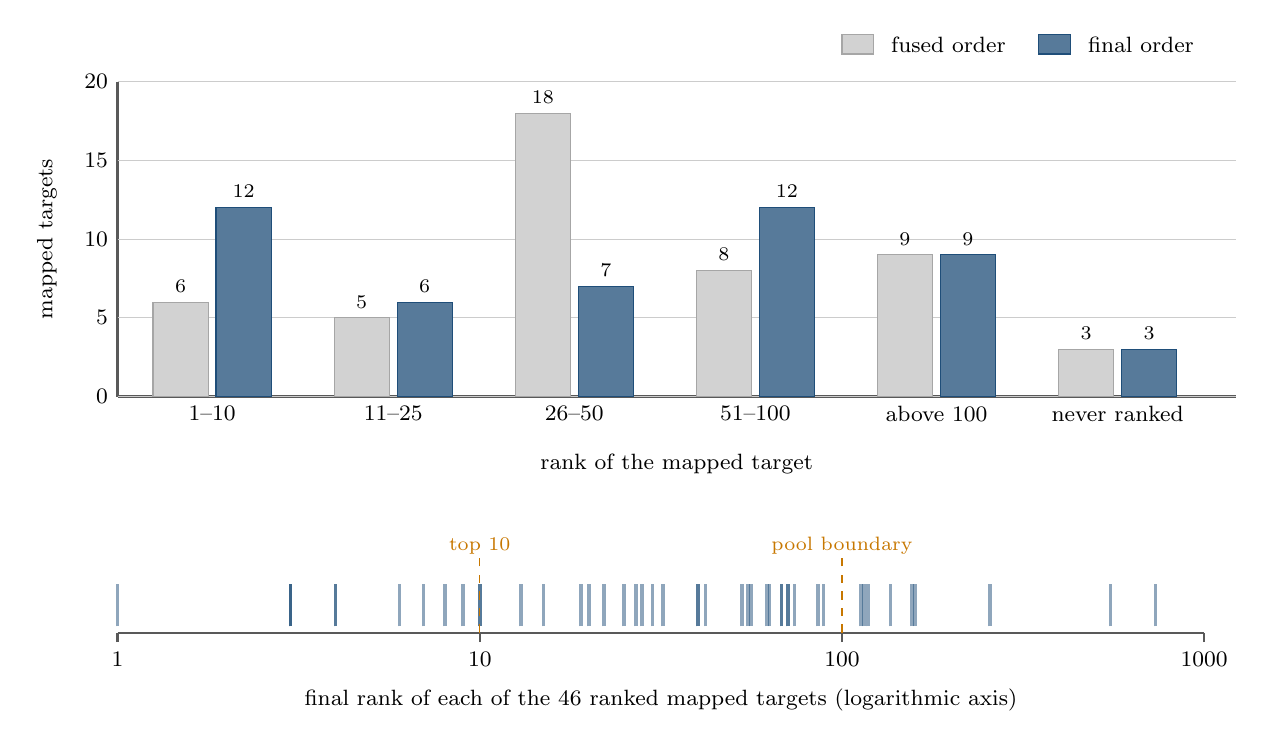
\begin{tikzpicture}[font=\footnotesize]
  \draw[vline] (0,0) -- (14.2,0);
  \draw[vline] (0,0) -- (0,4.0);
  \foreach \y/\lab in {0/0,1/5,2/10,3/15,4/20}{
    \draw[gray!40] (0,\y) -- (14.2,\y);
    \node[left] at (0,\y) {\lab};
  }
  \node[rotate=90] at (-0.9,2.0) {mapped targets};
  % scale: 0.2 cm per target
  \foreach \x/\nb/\na/\lab in {1.2/6/12/{1--10},3.5/5/6/{11--25},5.8/18/7/{26--50},8.1/8/12/{51--100},10.4/9/9/{above 100},12.7/3/3/{never ranked}}{
    \pgfmathsetmacro{\hb}{\nb*0.2}
    \pgfmathsetmacro{\ha}{\na*0.2}
    \draw[draw=gray!70,fill=gray!35] (\x-0.75,0) rectangle (\x-0.05,\hb);
    \draw[draw=accent,fill=accent!75] (\x+0.05,0) rectangle (\x+0.75,\ha);
    \node[below] at (\x,0) {\lab};
    \node[above,font=\scriptsize] at (\x-0.4,\hb) {\nb};
    \node[above,font=\scriptsize] at (\x+0.4,\ha) {\na};
  }
  \draw[draw=gray!70,fill=gray!35] (9.2,4.35) rectangle ++(0.4,0.25);
  \node[anchor=west] at (9.7,4.47) {fused order};
  \draw[draw=accent,fill=accent!75] (11.7,4.35) rectangle ++(0.4,0.25);
  \node[anchor=west] at (12.2,4.47) {final order};
  \node at (7.1,-0.85) {rank of the mapped target};
  % strip plot of final ranks on a log axis
  \begin{scope}[yshift=-3.0cm]
    \draw[vline] (0,0) -- (13.8,0);
    \foreach \rr in {1,10,100,1000}{
      \pgfmathsetmacro{\xx}{log10(\rr)*4.6}
      \draw[vline] (\xx,-0.12) -- (\xx,0);
      \node[below] at (\xx,-0.12) {\rr};
    }
    \foreach \rr in {1,3,3,3,4,4,6,7,8,9,10,10,13,15,19,20,22,25,27,28,30,32,40,40,42,53,55,56,62,63,68,68,71,71,74,86,89,113,115,118,136,156,159,256,551,733}{
      \pgfmathsetmacro{\xx}{log10(\rr)*4.6}
      \draw[accent,opacity=0.5,line width=1.3pt] (\xx,0.08) -- (\xx,0.62);
    }
    \pgfmathsetmacro{\xa}{log10(10)*4.6}
    \pgfmathsetmacro{\xb}{log10(100)*4.6}
    \draw[warnline,dashed] (\xa,0) -- (\xa,0.95);
    \draw[warnline,dashed] (\xb,0) -- (\xb,0.95);
    \node[text=warnline,font=\scriptsize] at (\xa,1.1) {top 10};
    \node[text=warnline,font=\scriptsize] at (\xb,1.1) {pool boundary};
    \node at (6.9,-0.85) {final rank of each of the 46 ranked mapped targets (logarithmic axis)};
  \end{scope}
\end{tikzpicture}}
\caption[Rank distribution of mapped targets (development diagnostics)]{\textbf{Development diagnostics.} Rank distribution of the 49 directly mapped
targets. Top: counts per rank band before reranking (grey) and after it (blue). The
cross-encoder moves mass out of the 26--50 band in both directions: into the top ten and
into the 51--100 band. The last two bands are identical by construction, since reranking
touches only the first 100 positions. Bottom: each ranked target's final position as one
tick on a logarithmic axis; darker ticks are coincident ranks. Nine ticks lie beyond the
pool boundary and were never seen by the cross-encoder.}
\label{fig:rank-dist}
\end{figure}

\subsection{Per-question view}

\begin{table}[!htbp]
\centering
\caption[Per-question results (development diagnostics)]{\textbf{Development diagnostics} per Type-A question for A6 ($K=100$). ``Mapped''
is the number of targets with a direct graph identity; ``union'' and ``pool'' count how
many of those survive each admission step; ``first'' is the best final rank of a mapped
target.}
\label{tab:per-question}
\small
\begin{tabular}{lrrrrrr}
\toprule
Question & Targets & Mapped & In union & In pool & Top 10 & First\\
\midrule
Q1 & 7 & 7 & 7 & 6 & 1 & 3\\
Q2 & 3 & 2 & 2 & 2 & 2 & 7\\
Q3 & 2 & 1 & 1 & 1 & 1 & 3\\
Q4 & 3 & 2 & 2 & 2 & 0 & 40\\
Q5 & 2 & 0 & 0 & 0 & 0 & --\\
Q6 & 3 & 1 & 1 & 1 & 0 & 22\\
Q7 & 2 & 1 & 1 & 1 & 0 & 71\\
Q8 & 2 & 1 & 1 & 1 & 1 & 6\\
Q9 & 3 & 1 & 1 & 0 & 0 & 256\\
Q10 & 2 & 1 & 1 & 0 & 0 & 156\\
Q11 & 2 & 0 & 0 & 0 & 0 & --\\
Q12 & 13 & 13 & 13 & 13 & 3 & 4\\
Q13 & 8 & 8 & 8 & 2 & 0 & 62\\
Q14 & 11 & 11 & 8 & 8 & 4 & 1\\
\midrule
Total & 63 & 49 & 46 & 37 & 12 & \\
\bottomrule
\end{tabular}
\end{table}

The aggregate hides strong concentration. Q12 and Q14 hold 24 of the 49 mapped targets
and 7 of the 12 top-ten hits. Six of the 14 questions have a mapped target in the top ten;
ten have one in the top 100. Q13 is the clearest admission failure: all eight of its
targets reach the union, but six are fused below rank 100. \Mtag

% ==================================================================
\section{Interpreting the Results}
\label{sec:interpretation}
% ==================================================================

\subsection{What A6 demonstrates}

\begin{itemize}
  \item \textbf{Entity-centric, multi-channel retrieval admits answer identities that
        entity-level dense retrieval alone does not.} Within the same entity universe, the
        dense lists cover 19 and 21 of 49 mapped targets, the evidence-owner list 44, and
        the union 46 (\cref{tab:coverage}). \Otag
  \item \textbf{Evidence-to-entity retrieval is the mechanism that addresses the original
        failure.} The texts that used to outrank the answer now carry their similarity to
        it. The worked example shows this for an entity that dense retrieval cannot see at
        all.
  \item \textbf{A cross-encoder allows deeper query--candidate interaction and improves
        the head of the list on this benchmark}: hits at 10 rise from 6 to 12 on the same
        pool. \Otag
  \item \textbf{The pipeline is auditable.} Every final rank can be traced to channel
        ranks, a fusion sum, a card with logged inclusions and omissions, a token count
        and a logit.
\end{itemize}

\subsection{What A6 does not demonstrate}

\begin{itemize}
  \item \textbf{It does not solve the task.} The system still misses most expected
        answers at useful depths: 51 of 63 are outside the top ten and the first result
        is a mapped target for one question out of 14.
  \item \textbf{Exact answer ranking remains difficult.} Most of the loss is in ordering
        (\cref{fig:result-funnel}), and the reranker also demotes admitted targets
        (\cref{tab:rerank-effect}).
  \item \textbf{No held-out claim.} Benchmark exposure makes these development results.
        The pool depth in particular was fixed with them in view.
  \item \textbf{No statistical claim.} Fourteen questions, one run, no intervals. A
        difference of a few hits is within what a handful of questions can produce.
  \item \textbf{No claim about the hierarchy.} V2 does not use it.
  \item \textbf{No comparison with V1 on equal terms.} V1 ranked 5{,}480 node documents and
        V2 ranks at most 2{,}577 eligible canonical entities with a different scoring
        rule. The two were not run as a matched experiment, so their numbers should not
        be subtracted from each other.
\end{itemize}

\begin{cautionbox}[Agreement with gold is not correctness, and disagreement is not error]
A high-ranked candidate that is not an annotated target has not been shown to be wrong.
The expected-method lists are short and were not written as exhaustive; several
high-ranked non-credited entities in \cref{tab:worked-final} are plausible answers or
duplicates of credited ones. Equally, a credited target at rank 4 does not show that the
system ``understood'' the question. Only an expert judgement of the returned lists could
settle either point, and none was made.
\end{cautionbox}

\subsection{Verified versus assumed}

\Cref{tab:verified} sorts the statements of this report by the kind of support they have.

\begin{table}[H]
\centering
\caption[Verified versus assumed]{Separation of what was verified from what was assumed or chosen.}
\label{tab:verified}
\small
\begin{tabularx}{\linewidth}{XX}
\toprule
Verified (read from frozen artifacts, or enforced and tested in code) & Assumed, chosen or not established\\
\midrule
Candidate counts: 46/49 in the union, 37/49 in the pool & That the answer-family map reflects what question authors mean\\
Top-$k$ recovery: 1, 6, 12, 18, 25, 37 of 63 & That $K=100$ is a good operating point beyond this benchmark\\
Prediction hash equal at freeze, evaluation and replay & That the graph path restrictions keep the right paths\\
Graph and index counts (\cref{tab:index}) & That the evidence caps show the most useful evidence\\
Pinned model revisions and file hashes & That a web-search relevance model is a useful prior for materials-science method selection\\
0 denied reads, 0 gold reads during prediction & That node types and years in the source data are correct\\
57 tests passed & That the target mapping is complete and correct (no expert adjudication)\\
Reranking permutes only the first 100 positions & That non-credited high-ranked candidates are wrong (not established)\\
Evaluator recovers 49/49 forced identities & Held-out generalisation; month-level temporal validity\\
\bottomrule
\end{tabularx}
\end{table}

% ==================================================================
\section{Efficiency}
\label{sec:efficiency}
% ==================================================================

The two-stage design is motivated by cost, so the cost should be stated. The run is a
single CPU process with four threads. \Cref{tab:efficiency} lists the logical work per
question, and \cref{fig:efficiency} shows where it goes.

\begin{table}[!htbp]
\centering
\caption[Logical work and timing]{Logical work per question, and timing where the frozen run recorded it. Counts
are comparisons, not latency. \Mtag{} Sources: \code{audit/efficiency.json} and
\code{evaluation/efficiency\_report.json}.}
\label{tab:efficiency}
\small
\begin{tabularx}{\linewidth}{p{4.3cm}p{4.6cm}X}
\toprule
Operation & Per question & Note\\
\midrule
Dense inner products & 10{,}960 (5{,}480 documents $\times$ 2 views) & The run also scored a
  third, diagnostic view not used in fusion; logged total 16{,}440\\
Evidence inner products & 8{,}548 (4{,}274 items $\times$ 2 views) & Reused by the evidence
  channel, the graph channel and card selection\\
BM25 & 2{,}978 lexical documents & 1{,}637{,}900 document-term lookups over 18 questions\\
Name checks & one per eligible entity & at most 2{,}978\\
Graph expansion & 200 seeds, fan-out $\le64$, $\le2$ hops & bounded by construction\\
\midrule
Cross-encoder pairs & \textbf{100} & 1{,}800 over 18 questions\\
Cross-encoder time, 100 pairs & 7.7 s mean (3.8 to 11.4 s) & Sum of logged amortised batch
  times for the first 100 fused candidates; an estimate\\
First-stage time & 0.83 s mean (0.14 to 1.13 s) & With corpus vectors already cached;
  includes trace writing\\
\bottomrule
\end{tabularx}
\end{table}

\begin{figure}[!htbp]
\centering
\fitfig{%
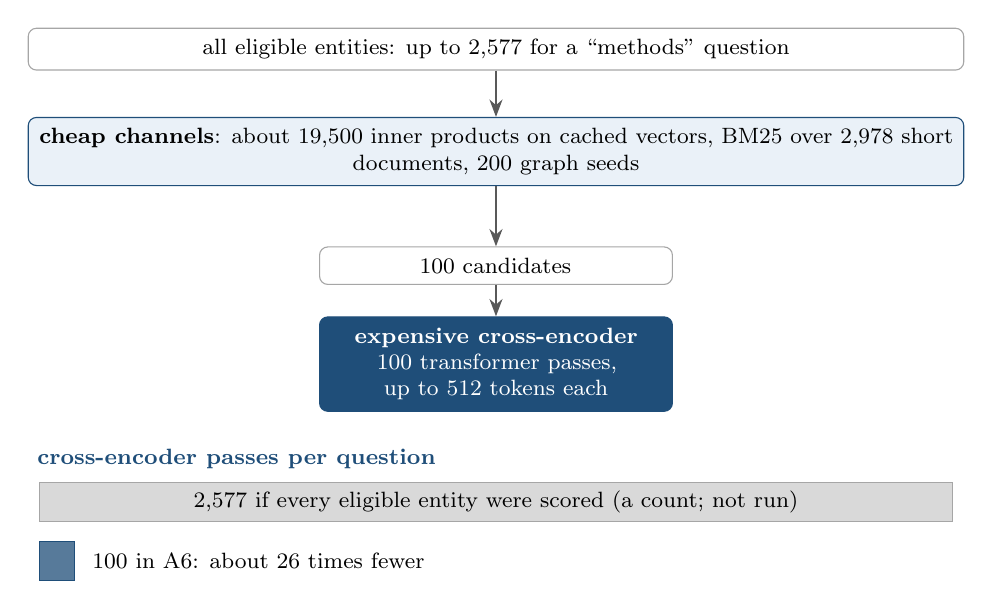
\begin{tikzpicture}[font=\footnotesize]
  \node[vplain,text width=11.6cm] (a) at (0,0) {all eligible entities: up to 2{,}577 for a ``methods'' question};
  \node[vbox,text width=11.6cm] (b) at (0,-1.3) {\textbf{cheap channels}: about 19{,}500 inner products on cached vectors,
     BM25 over 2{,}978 short documents, 200 graph seeds};
  \node[vplain,text width=4.2cm] (c) at (0,-2.75) {100 candidates};
  \node[vdark,text width=4.2cm] (d) at (0,-4.0) {\textbf{expensive cross-encoder}\\ 100 transformer passes,\\ up to 512 tokens each};
  \draw[varr] (a)--(b); \draw[varr] (b)--(c); \draw[varr] (c)--(d);
  \node[anchor=west,font=\footnotesize\bfseries,text=accent] at (-5.95,-5.2) {cross-encoder passes per question};
  \draw[draw=gray!70,fill=gray!30] (-5.8,-6.0) rectangle ++(11.6,0.5);
  \node at (0,-5.75) {2{,}577 if every eligible entity were scored (a count; not run)};
  \draw[draw=accent,fill=accent!75] (-5.8,-6.75) rectangle ++(0.45,0.5);
  \node[anchor=west] at (-5.25,-6.5) {100 in A6: about 26 times fewer};
\end{tikzpicture}}
\caption[Cheap first stage, expensive second stage]{Where the work goes. The first stage touches every eligible entity but only with
operations on precomputed vectors and term statistics. The cross-encoder is confined to
100 candidates. The bars compare the number of joint forward passes per question with and
without the first stage; the longer bar is a count, not an experiment that was run.}
\label{fig:efficiency}
\end{figure}

Three cautions apply.
\begin{itemize}
  \item \textbf{Comparisons are not production latency.} They count operations; they say
        nothing about batching, hardware or serving overhead.
  \item \textbf{CPU timing is machine-specific.} The times are from one CPU run on one
        machine and mix cached and uncached work. The 100-pair time is assembled from amortised
        batch timings of a run that scored a deeper prefix; it was not measured as a
        stand-alone 100-pair run.
  \item \textbf{Nothing here is a scalability claim.} The corpus is 52 papers. Exhaustive
        inner products and a pure-Python BM25 are adequate at this size and would need
        replacing at a larger one.
\end{itemize}

% ==================================================================
\section{Reproducibility}
\label{sec:repro}
% ==================================================================

\begin{table}[!htbp]
\centering
\caption[Pinned models and environment]{Pinned models and environment of the frozen run. \Mtag{} Sources:
\code{config.json}, \code{model\_manifest.json} and
\code{audit/model\_version\_manifest.json}.}
\label{tab:env}
\small
\begin{tabularx}{\linewidth}{p{3.6cm}X}
\toprule
Item & Value\\
\midrule
Bi-encoder & \code{BAAI/bge-small-en-v1.5}\\
\quad revision & \code{5c38ec7c405ec4b44b94cc5a9bb96e735b38267a}\\
Cross-encoder & \code{cross-encoder/ms-marco-MiniLM-L6-v2}\\
\quad revision & \code{233902d25c440f23af6f7d6e94d2946bac0bee0a}\\
Model files & every file hashed (SHA-256) in the manifest and checked before prediction\\
Python & 3.11.2 (Windows, 64-bit)\\
Libraries & numpy 2.3.5; torch 2.4.1; transformers 4.57.6; sentence-transformers 5.1.0; huggingface-hub 0.36.2\\
Device & CPU, 4 threads; offline mode, local files only\\
Seed & 42 for Python, NumPy and PyTorch; deterministic algorithms enforced\\
Batch sizes & 32 (encoder), 16 (cross-encoder)\\
Full dependency closure & \path{requirements.txt} (exact versions)\\
\bottomrule
\end{tabularx}
\end{table}

\paragraph{Determinism.} Every sort has an explicit tie-breaker (entity id, evidence id or
seed id). Fusion accumulates channels in sorted name order. BM25 iterates over query terms
in sorted order, so its floating-point sums do not depend on Python's hash seed (tested by
\path{test_bm25_independent_of_python_hash_seed}). No sampling occurs anywhere.

\paragraph{Frozen artifacts.} The freeze manifest covers 155 files. A second execution of
the predictor into a separate directory reproduced the predictions byte for byte, with the
same SHA-256 (\cref{sec:leakage}); it reused cached model outputs. \Mtag

\paragraph{Process separation.} Prediction and evaluation are different entry points
(\path{scripts/predict.py}, \path{scripts/evaluate.py}). The predictor refuses to overwrite
an existing freeze; a new run must name a new output directory.

\paragraph{Tests.} The V2 suite has 57 tests; all passed, none failed. \Mtag{} The suite
covers the whole V2 package, including parts outside this document's scope. Those most
relevant to A6 are listed in \cref{tab:tests}.

\begin{table}[!htbp]
\centering
\caption[Tests guarding the properties relied upon]{Tests that guard the properties this document relies on (names as in the
repository).}
\label{tab:tests}
\small
\begin{tabularx}{\linewidth}{p{10.4cm}X}
\toprule
Test & Property\\
\midrule
\path{test_grouping_deterministic_and_no_fuzzy_alias_merges} & Canonical entities\\
\path{test_temporal_visibility_applies_to_nodes_edges_aliases} & Visibility\\
\path{test_safe_names_match_boundaries_and_punctuation} & Name channel\\
\path{test_graph_bounded_paths_and_hubs} & Graph caps and path shapes\\
\path{test_rrf_is_rank_only_and_order_independent} & Fusion\\
\path{test_query_dependent_selection_and_deduplication} & Card selection\\
\path{test_identity_survives_token_packing} & Identity kept in the card\\
\path{test_all_cross_encoder_identities_and_token_limits} & 512-token limit\\
\path{test_reranker_only_changes_frozen_prefix} & Head/tail rule\\
\path{test_prediction_source_has_no_gold_or_evaluator_import} & Isolation\\
\path{test_runtime_guard_blocks_protected_writes_and_gold_reads} & Isolation\\
\path{test_evaluation_freeze_refuses_tampering} & Freeze\\
\path{test_full_cached_replay_is_identical_when_available} & Replay\\
\bottomrule
\end{tabularx}
\end{table}

\paragraph{Commands.} From the repository root, in PowerShell. These are the README's
commands with the interpreter path abbreviated as \code{\$py}.

{\footnotesize
\begin{verbatim}
python -m venv clean_tshc_v2/.venv
$py = "clean_tshc_v2/.venv/Scripts/python.exe"
& $py -m pip install -r clean_tshc_v2/requirements.txt
& $py -B clean_tshc_v2/scripts/prepare_models.py
& $py -B clean_tshc_v2/scripts/predict.py
& $py -B clean_tshc_v2/scripts/evaluate.py
& $py -B clean_tshc_v2/scripts/predict.py --output artifacts/reproduction
& $py -B -m pytest clean_tshc_v2/tests -q -p no:cacheprovider
\end{verbatim}
}

\noindent Model preparation uses local files unless run with \code{--download}; it never
substitutes a different revision. The A6 ranking with $K=100$ is the entry
\code{rankings["A6\_100"]} of each question in
\path{artifacts/prediction/retrieval/predictions.json}, and its metrics are under
\code{systems["A6\_100"]} in \path{artifacts/evaluation/metrics.json}.

% ==================================================================
\section{Limitations}
\label{sec:limitations}
% ==================================================================

\begin{cautionbox}[The three limitations that matter most]
\begin{enumerate}[leftmargin=*]
  \item \textbf{Development benchmark.} The questions and answers were seen during design.
        Nothing here measures performance on unseen questions.
  \item \textbf{Incomplete and unadjudicated gold.} Fourteen of 63 targets have no direct
        graph identity, and a high-ranked non-gold candidate is not known to be wrong.
  \item \textbf{General-purpose relevance model on thin evidence.} The reranker was
        trained on web search, and most entities have almost no evidence to show it.
\end{enumerate}
\end{cautionbox}

The complete list:

\begin{enumerate}
  \item \textbf{Development benchmark, not held out.} Earlier iterations were evaluated on
        the same questions; run-time isolation does not undo that.
  \item \textbf{Small number of scored questions.} Fourteen Type-A questions, 63 target
        occurrences, one deterministic run, no confidence intervals. Two questions hold
        about half of the mapped targets (24 of 49).
  \item \textbf{Some gold entities are PARTIAL, ABSENT or COMPOSITE.} They can never earn
        direct credit, capping recall at $49/63$.
  \item \textbf{Hard answer-type filtering can exclude valid entities} when the graph's
        typing disagrees with the question's wording. Three expected datasets were removed
        this way.
  \item \textbf{Entity-specific evidence coverage is incomplete.} 2{,}508 of 2{,}978
        entities have article titles only. The conservative safe-name rule adds to this:
        names such as ``CHGNet'' are not recognised as identifiers and gain no mention
        evidence.
  \item \textbf{The cross-encoder is trained on general relevance data}, not on
        materials-science method selection. It rewards restatement of the question
        (\cref{tab:worked-final}).
  \item \textbf{Relevance logits are not calibrated probabilities.} They order candidates
        within one question and mean nothing across questions.
  \item \textbf{Evidence associated through graph structure does not entail a scientific
        claim.} Most graph paths are citation paths.
  \item \textbf{Year-only dates cannot enforce ``February 2026''.}
  \item \textbf{A high-ranked non-gold candidate is not demonstrated to be wrong.}
  \item \textbf{$K=100$ is a development configuration.} Among the predeclared reranking
        depths it gave the strongest observed top-10 recovery, and it was selected after
        the development results were available. It is not the frozen run's primary
        configuration and not an independently validated or universal optimum.
  \item \textbf{No model fine-tuning was performed}, by design and in line with the
        assessment's scope. A domain-adapted reranker might behave differently.
  \item \textbf{No claim of production latency or scalability} beyond this 52-paper
        corpus.
  \item \textbf{Conservative identity grouping fragments answers.} Near-identical entities
        with different surface forms are ranked and scored separately.
  \item \textbf{The structured view comes from a heuristic parser} that can mis-split a
        question; only the parallel verbatim view protects against this.
\end{enumerate}

% ==================================================================
\section{What Four More Weeks Would Add}
\label{sec:future}
% ==================================================================

None of the following has been implemented, and no result is claimed for any of it. In
priority order:

\begin{enumerate}
  \item \textbf{Independent expert evaluation of retrieved answers.} Have a domain expert
        judge the top results per question blind to the gold list. This replaces
        ``agreement with an incomplete list'' by an actual precision estimate and settles
        whether non-credited candidates are errors.
  \item \textbf{A genuinely held-out query set}, written before looking at any retrieval
        output, with the configuration (including $K$) fixed in advance.
  \item \textbf{Better graph evidence coverage.} Most entities have nothing
        candidate-specific to show. Linking more claims to the entities they describe,
        with the same role checks, would give both the evidence channel and the card
        something to work with.
  \item \textbf{Scientifically specialised reranking.} Evaluate a relevance model adapted
        to scientific text, declared before scoring, against the general-purpose one.
  \item \textbf{Softer or evidence-aware answer-family constraints}, so that an entity
        typed as a component but evidenced as a dataset is demoted instead of deleted.
  \item \textbf{Larger-corpus performance profiling}, to learn where exhaustive scoring
        stops being adequate.
  \item \textbf{Method-level answer synthesis}, only after entity retrieval is
        trustworthy. Generating prose answers on top of an unreliable ranking would hide
        its errors.
  \item \textbf{A matched comparison with hierarchy routing}, holding entities, evidence,
        scorers, snapshot, mapping and cost accounting fixed, so that the main report's
        open extrinsic question can be answered on equal terms.
\end{enumerate}

% ==================================================================
\section{Conclusion}
\label{sec:conclusion}
% ==================================================================

The main report showed that hierarchy construction can be evaluated rigorously, and its
initial downstream retriever exposed an answer-identity bottleneck: dense similarity found
the right scientific region and ranked the texts describing a solution above the name of
the solution.

V2 responds by separating two tasks. \emph{Candidate admission} uses complementary
semantic, lexical, evidence and graph signals over canonical entities to form a
high-recall pool, and reciprocal rank fusion combines their rankings without calibrating
their scores. \emph{Candidate ordering} applies a joint relevance cross-encoder, the one
expensive operation, to only the top 100 candidates, each presented as an identity-first,
query-dependent card of provenance-bearing evidence.

On the development benchmark the pool admits 37 of 49 mapped targets and the final ranking
places 12 of 63 targets in the top ten. The result is imperfect and development-only:
ordering loses more targets than admission, the reranker rewards restatement of the
question, evidence is thin, and the gold lists are incomplete. It is nevertheless an
auditable, reproducible retrieval architecture, with predictions frozen before scoring,
that directly addresses the failure exposed by the original extrinsic evaluation, and it
leaves the hierarchy and its guarantees exactly as the main report established them.

\section*{AI assistance}
\addcontentsline{toc}{section}{AI assistance}
This supplement was drafted with an AI writing assistant from the current V2 source and
the frozen artifacts listed in \cref{app:artifacts}; every number was read from those
artifacts. AI use in the V2 implementation is documented in \path{AI_USAGE.md} of the V2
package.

% ==================================================================
\addcontentsline{toc}{section}{References}
\begin{thebibliography}{99}
\setlength{\itemsep}{3pt}
\small

\bibitem[Bajaj et~al.(2016)]{bajaj2016msmarco}
P.~Bajaj, D.~Campos, N.~Craswell, L.~Deng, J.~Gao, X.~Liu, R.~Majumder, A.~McNamara,
B.~Mitra, T.~Nguyen, M.~Rosenberg, X.~Song, A.~Stoica, S.~Tiwary and T.~Wang.
\newblock MS MARCO: A human generated MAchine Reading COmprehension dataset.
\newblock \emph{arXiv:1611.09268}, 2016.

\bibitem[Burduli(2026)]{burduli2026tshc}
L.~Burduli.
\newblock Temporal Semantic Hypergraph Coarsening: Multi-resolution semantic abstraction
over an evolving knowledge hypergraph.
\newblock Technical research report, September 2026. Package \texttt{clean\_tshc},
file \texttt{report/full\_report.pdf}.

\bibitem[Cormack et~al.(2009)]{cormack2009rrf}
G.~V. Cormack, C.~L.~A. Clarke and S.~B\"uttcher.
\newblock Reciprocal rank fusion outperforms Condorcet and individual rank learning methods.
\newblock In \emph{Proc.\ 32nd Annual International ACM SIGIR Conference on Research and
Development in Information Retrieval}, pages 758--759, 2009.
\newblock doi:10.1145/1571941.1572114.

\bibitem[Devlin et~al.(2019)]{devlin2019bert}
J.~Devlin, M.-W. Chang, K.~Lee and K.~Toutanova.
\newblock BERT: Pre-training of deep bidirectional transformers for language understanding.
\newblock In \emph{Proc.\ 2019 Conference of the North American Chapter of the Association
for Computational Linguistics: Human Language Technologies, Volume 1 (Long and Short
Papers)}, pages 4171--4186, 2019.
\newblock doi:10.18653/v1/N19-1423.

\bibitem[Nogueira and Cho(2019)]{nogueira2019passage}
R.~Nogueira and K.~Cho.
\newblock Passage re-ranking with BERT.
\newblock \emph{arXiv:1901.04085}, 2019.

\bibitem[Reimers and Gurevych(2019)]{reimers2019sbert}
N.~Reimers and I.~Gurevych.
\newblock Sentence-BERT: Sentence embeddings using Siamese BERT-networks.
\newblock In \emph{Proc.\ EMNLP-IJCNLP}, pages 3982--3992, 2019.

\bibitem[Robertson and Zaragoza(2009)]{robertson2009bm25}
S.~Robertson and H.~Zaragoza.
\newblock The probabilistic relevance framework: BM25 and beyond.
\newblock \emph{Foundations and Trends in Information Retrieval}, 3(4):333--389, 2009.
\newblock doi:10.1561/1500000019.

\bibitem[Vaswani et~al.(2017)]{vaswani2017attention}
A.~Vaswani, N.~Shazeer, N.~Parmar, J.~Uszkoreit, L.~Jones, A.~N. Gomez, {\L}.~Kaiser and
I.~Polosukhin.
\newblock Attention is all you need.
\newblock In \emph{Advances in Neural Information Processing Systems 30}, 2017.

\bibitem[Wang et~al.(2020)]{wang2020minilm}
W.~Wang, F.~Wei, L.~Dong, H.~Bao, N.~Yang and M.~Zhou.
\newblock MiniLM: Deep self-attention distillation for task-agnostic compression of pre-trained
transformers.
\newblock In \emph{Advances in Neural Information Processing Systems 33}, 2020.

\bibitem[Xiao et~al.(2023)]{xiao2023bge}
S.~Xiao, Z.~Liu, P.~Zhang and N.~Muennighoff.
\newblock C-Pack: Packaged resources to advance general Chinese embedding.
\newblock \emph{arXiv:2309.07597}, 2023.

\end{thebibliography}

% ==================================================================
\clearpage
\appendix
\section{Configuration Constants}
\label{app:config}
% ==================================================================

\begin{table}[H]
\centering
\caption[Configuration constants]{Constants used by A6, from the frozen \code{config.json}. All are fixed
settings and none was fitted, except that the reranking depth $K$ was selected among
predeclared depths after development results were available (\cref{sec:k-status}). \Dtag}
\label{tab:config}
\small
\begin{tabularx}{\linewidth}{p{5.0cm}p{3.2cm}X}
\toprule
Field & Value & Role\\
\midrule
\code{snapshot} & 2026 & Latest visibility cutoff\\
\code{seed}, \code{threads} & 42, 4 & Determinism and CPU threads\\
\code{context\_cap} & 12 & Neighbours in a dense node document\\
\code{bm25\_k1}, \code{bm25\_b} & 1.5, 0.75 & BM25 saturation and length normalisation\\
\code{channel\_depth} & 500 & Truncation of each first-stage list\\
\code{evidence\_seed\_depth} & 500 & Evidence seeds for the evidence channel\\
\code{graph\_seed\_depth} & 200 & Evidence seeds for graph expansion\\
\code{graph\_max\_hops} & 2 & Maximum path length\\
\code{graph\_fanout\_cap} & 64 & Arcs followed from one node\\
\code{graph\_article\_degree\_cap} & 80 & Largest article usable as an intermediate\\
\code{graph\_path\_decay} & 0.8 & Factor per hop beyond the first\\
\code{rrf\_k} & 60 & Fusion constant\\
\code{cross\_encoder\_max\_tokens} & 512 & Input limit of the reranker\\
\code{query\_evidence\_caps} & see \cref{tab:caps} & Blocks per evidence family\\
\code{answer\_families} & see \cref{tab:families} & Answer head to node types\\
Reranking pool $K$ & 100 & Ranking key \code{A6\_100}. The field \code{rerank\_k}${}=500$ is the
  frozen run's primary depth; 100 is one of its declared \code{rerank\_controls}, selected
  after development results were available\\
\bottomrule
\end{tabularx}
\end{table}

% ==================================================================
\section{Artifacts and Sources Inspected}
\label{app:artifacts}
% ==================================================================

Every numerical or implementation statement in this document was taken from the files
below, in this order of precedence: frozen prediction and evaluation artifacts; current V2
source and configuration; current V2 README and reports; the main report for inherited
hierarchy properties. No experiment was run and no file other than this document was
written.

\begin{table}[H]
\centering
\caption[Sources inspected]{Sources, relative to \code{clean\_tshc\_v2/} unless stated.}
\label{tab:artifacts}
\small
\begin{tabularx}{\linewidth}{p{7.4cm}X}
\toprule
File & Used for\\
\midrule
\path{artifacts/evaluation/metrics.json} & Recall, MRR, candidate recall, status counts, channel coverage, reranking movement\\
\path{artifacts/evaluation/per_question_evaluation.json} & Per-question and per-target ranks\\
\path{artifacts/evaluation/efficiency_report.json} & Logical work totals\\
\path{artifacts/evaluation/audit/evaluation_manifest.json} & Hashes at evaluation\\
\path{artifacts/prediction/retrieval/predictions.json} & Fused and final rankings\\
\path{artifacts/prediction/retrieval/channels/} & Per-channel ranks, scores, graph paths\\
\path{artifacts/prediction/retrieval/selected_evidence/} & Selected and omitted card evidence\\
\path{artifacts/prediction/retrieval/cross_encoder/} & Packed blocks, token counts, logits\\
\path{artifacts/prediction/query_understanding/} & Query views, answer heads, cutoffs\\
\path{artifacts/prediction/entity_index/2026.json} & Entities, evidence links, arcs\\
\path{artifacts/prediction/audit/} & Freeze manifest, event log, access audit, efficiency, model versions\\
\path{artifacts/reproduction/retrieval/predictions.sha256} & Replay hash\\
\path{artifacts/verification/} & Test log, final verification\\
\path{config.json}, \path{model_manifest.json}, \path{requirements.txt} & Constants, revisions, hashes, versions\\
\path{src/tkh_abstraction_v2/*.py}, \path{scripts/predict.py}, \path{scripts/evaluate.py} & Implementation behaviour\\
\path{tests/*.py} & Test names\\
\path{README.md}, \path{notes/ASSESSMENT_ALIGNMENT.md}, \path{report/} & Commands, scope, existing V2 reports\\
\path{../clean_tshc/report/full_report.tex} & Inherited hierarchy properties, V1 retrieval result, style\\
\path{../clean_tshc/data/ASSESSMENT.md} & P1--P6, T1--T7, scoring weights\\
\bottomrule
\end{tabularx}
\end{table}

% ==================================================================
\section{Glossary}
\label{app:glossary}
% ==================================================================

\begin{description}[leftmargin=0.6cm,style=nextline,itemsep=1pt]
  \item[A6] The configuration described here: fused candidates reranked by a relevance
        cross-encoder; pool $K=100$.
  \item[Answer family] The node types admitted for a question's answer head.
  \item[Bi-encoder] A model that embeds each text separately; scoring is a vector product.
  \item[BM25] A lexical scoring function based on term frequency, inverse document
        frequency and length normalisation.
  \item[Candidate card] The text shown to the cross-encoder for one candidate: identity,
        then selected evidence.
  \item[Candidate pool] The first $K$ entities of the fused order; the only entities the
        cross-encoder scores.
  \item[Canonical entity] An equivalence class of graph nodes with the same normalised
        name in a compatible type family.
  \item[Cross-encoder] A model that reads question and candidate jointly and outputs one
        score.
  \item[Evidence item] A claim, task, problem, technique, component, dataset, metric or
        article node whose text can support an entity.
  \item[Freeze] Hashing predictions and their traces before the evaluator may run.
  \item[Relevance logit] The cross-encoder's unbounded output; an ordering signal, not a
        probability.
  \item[RRF] Reciprocal rank fusion: a sum of $1/(k+\text{rank})$ over lists.
  \item[Seed] One of the evidence items most similar to the question, from which the
        evidence and graph channels start.
  \item[TKH] Temporal Knowledge Hypergraph, the supplied data.
\end{description}

\end{document}
